\documentclass[english, LaM, oneside, noexaminfo]{sapthesis}
%Bachelor's (laurea triennale) thesis : Lau 
%Master's (laurea specialistica) thesis: LaM 
%PhD's thesis: PhD 

% PACCHETTI DA SAPHTHESIS
\usepackage[utf8]{inputenx}
\usepackage{indentfirst}
\usepackage{microtype}
\usepackage{amsfonts}
\usepackage{lettrine}
\linespread{0.9}
\usepackage[nottoc, notlof, notlot]{tocbibind}

% PACCHETTI INSERITI DA ME
\usepackage{tikz,pgf}   % feynman diagrams
\usepackage{tikz-feynman,contour}   % feynman diagrams
\usepackage{biblatex}   % my version of bibliography
\addbibresource{include-LaTex-MScThesis/MSc_bibliography.bib}
\bibstyle{unsrt}
\usepackage{scrextend}  % noindent footnote
\deffootnote{2em}{0em}{\thefootnotemark\quad}
\usepackage{simpler-wick}
\usepackage{caption}
\usepackage{subcaption}
\usepackage{slashed}
\usepackage{amssymb}

\usepackage{hyperref}
\hypersetup{
			hyperfootnotes=true,			
			bookmarks=true,			
			colorlinks=true,
            filecolor = black,
			linkcolor=black,
            linktoc=page,
			anchorcolor=black,
			citecolor=black,
			urlcolor=black,
			pdftitle={tesiM},
			pdfauthor={FirstName LastName},
			pdfkeywords={thesis, sapienza, roma, university}
}

% customized commands
\newcommand{\kkb}{$K^0$ - $\bar K^0$ }
\newcommand{\la}{\langle}
\newcommand{\ra}{\rangle}
\newcommand{\colg}{\textcolor{gray}}
\newcommand{\colr}{\textcolor{red}}
\newcommand{\colv}{\textcolor{violet}}
\newcommand{\bare}{^{\text{bare}}}
\newcommand{\ren}{{\text{ren}}}
\newcommand{\cpt}{$\chi\text{PT}$}
\newcommand{\mev}{\text{ MeV}}
\newcommand{\gev}{\text{ GeV}}
\newcommand{\fm}{\text{ fm}}
\newcommand{\oaid}{$O(a)-$improved}
\newcommand{\oait}{$O(a)-$improvement}
\newcommand{\obc}{Open Boundary Conditions}
\newcommand{\tr}{\text{Tr}}
\newcommand{\spc}{\hspace*{1mm}}
\newcommand{\proved}{\newline \hspace*{.97\textwidth} $\square$}

\title{Non-perturbative computation of Kaons oscillation amplitudes in Lattice Quantum Chromodynamics with $N_f = 2+1$ sea quarks and Open Boundary Conditions}
\author{Emanuele Rosi}
\IDnumber{1812180}
\course[]{Fisica Teorica}
\courseorganizer{Facolt\`a di Scienze Matematiche Fisiche e Naturali}
\submitdate{2022/2023}
\copyyear{2023}
\advisor{Prof. Mauro L. Papinutto}
\authoremail{rosiemanuele99@gmail.com}
\examdate{data da stabilire}
\examiner{Prof. ...} \examiner{Prof. ...} \examiner{Prof. ...}  \examiner{Prof. ...}  \examiner{Prof. ...} \examiner{Prof. ...}  \examiner{Prof. ...} 

\begin{document}
\frontmatter
\maketitle

\dedication{
    \hspace*{.76\textwidth}Ai miei genitori.
    \newline
    \newline
    \newline
    \newline
    A tutte quelle giornate in cui non mi stavo sacrificando per lo studio, stavo facendo ciò che amo.
}

\begin{abstract}
    Oscillations of neutral Kaons are a well known phenomenon within the framework of the Standard Model (SM) of particle physics.
    These oscillations arise from quark flavor mixing governed by the Cabibbo-Kobayashi-Maskawa matrix in weak interactions.
    Furthermore, decay rates of the Kaons are studied to get an indirect measure of $CP$ violation in the Standard Model, quantified through the parameter $\epsilon_K$ \cite{Branco-CPviolation}.
    Precise theoretical predictions are essential.
    As I have implicitly mentioned, the Kaons oscillation phenomenon takes place at low energies, where the quarks are confined in mesons and baryons - energies of order of $\Lambda_\text{QCD} \sim 250$\mev\space \cite{WeinbergII}.
    Perturbation theory (PT) represents the most powerful tool of theoretical physicists to understand the world of particle physics.
    However it imposes the requirement of energies much higher than $\Lambda_\text{QCD}$, requirement not satisfied in the energetic region concerning confinement.
    The PT approach becomes inefficient and the only other valid approach to QFT is the path integral formalism.
    Usually, direct calculations in path integral are performed through lattice QFT simulations.
    \newline
    In this work I treat a set of dimension 6 four-quarks operators responsible for the oscillations of neutral Kaons.
    They constitute an effective Hamiltonian for the oscillating system
    $$ \mathcal{H}^{\Delta S=2}_\text{eff,BSM} = \sum_i \hat C_i (\mu) \hat\Theta_i (\mu) $$
    The first operator $\hat\Theta_1$ is the effective operator associated to the SM contribution to the oscillations.
    The others take place in beyond the standard model (BSM) theories, such as supersymmetry or multi Higgs models \cite{Bparameters}.
    The purpose is to compute parameters associated to the bare Kaon oscillation amplitudes caused by each $\Theta_i$ operator:
    $$ \mathcal{A}_i^\text{QCD} = \la \bar K^0 | \Theta_i\bare | K^0 \ra $$
    Such quantities are called {\it bag parameters} \cite{Bparameters} \cite{KMBSM}.
    The renormalization of such operators and parameters is not involved in this work and it is developed in some papers, such as \cite{renrun}.
    $B$-parameters are widely studied in the context of lattice QCD (LQCD) and results of the most recent works can be found in \cite{FLAG}.
    \newline
    Lattice simulations suffer from an amount of computational issues such as finite spacetime volume effects or lattice spacing effects.
    The lattice setup chosen for this work aims to minimize some of these effects. 
    Firstly, there is a computational problem in the generation of gauge configurations; ideally, they should be totally uncorrelated from each other, but their autocorrelation times grow as the lattice spacing is reduced. \cite{critical-slowing-down-error-analysis}
    It is proven that this problem is partially solved by choosing open boundary conditions in temporal direction. \cite{OBC_top}
    Secondly, these boundary conditions protect the fermion determinant from the occurrence of zero eigenvalues of the Wilson-Dirac operator \cite{SF-luscher}.
    In this sense open boundary conditions give an efficient alternative to twisted mass QCD (tmQCD) \cite{tmLQCD} - used in \cite{KMBSM} - and allow the simulation program to simulate three flavours of sea quarks, not allowed in tmQCD.
    The entire simulation is developed to yield \oaid\space results, i.e. values that differ from the continuum limit ones by terms of order $O(a^2)$ or higher.
    This is possible thanks to the strategy worked out by Frezzotti and Rossi in \cite{FR2}.
    Such strategy involves maximally twisted Osterwalder-Seiler quarks in the valence sector.
    Further properties of the lattice mixing operators are well explained in \cite{DoniniMartinelliOperators}, such as their mixing pattern under renormalization procedure.
    \newline
    The thesis is structured as follows.
    The first chapter covers basic concepts of Standard Model QCD, confinement, pseudoscalar mesons, and Kaon oscillations.
    Moreover I introduce the bag parameters and the complete set of mixing operators $\{\Theta_i\}$.
    The second chapter provides an overview of lattice regularizations and improvements;
    I begin from the basics - Wilson-Dirac action and Wilson Gauge action - and I describe some of their related problems (zero modes, long autocorrelation times, exceptional configurations, $O(a)$ efficiency).
    Then a description of more advanced regularizations follows.
    At the end of the chapter I outline the adopted lattice setup as a solution of almost all the presented problems.
    The chapter \ref{ch:operators} is completely dedicated to the construction of three points correlators on the lattice.
    The operators $\Theta_i$ are described in continuum theory, then they are regularized on the lattice by following the strategy in \cite{FR2}.
    All the properties are described in detail and most of them are proven. At the end of the chapter I describe the analysis of the asymptotic behaviour of the correlation functions at large Euclidean time, widely used in QFT.
    In the fourth chapter I present the computational strategies developed to calculate the needed Wick contractions of the two and three points correlators.
    Particular relevance is given to the calculation of three points correlators through the method of noise spinors, that represents most of the ``behind the scenes'' thesis work.
    A conclusive section provides the reader information about the status of the simulation and reports the achievements of this work.
\end{abstract}

\tableofcontents

\mainmatter

%%%%%%%%%%%%%%%%%%%%%%%%%%%%%%%%%%%%%%%%%%%%%%%%%%%%%%%%%%%%%%%%%%%%%%%%%%%%%%%%%%%%%%%%%
%%%%%%%%%%%%%%%%%%%%%%%%%%%%%%%%%%%%% FIRST CHAPTER %%%%%%%%%%%%%%%%%%%%%%%%%%%%%%%%%%%%%
%%%%%%%%%%%%%%%%%%%%%%%%%%%%%%%%%%%%%%%%%%%%%%%%%%%%%%%%%%%%%%%%%%%%%%%%%%%%%%%%%%%%%%%%%
\chapter{Kaons oscillations beyond the Standard Model and $B_i$ parameters}\label{chap:kaons}
\lettrine[lines=2, findent=3pt, nindent=0pt]{I}{}n order to present and justify my work, I begin the thesis with an introductive chapter about theory of \kkb system within the Standard Model (SM) of particle physics and beyond. 
Firstly, I present the Standard Model \kkb oscillations.
Then I discuss oscillations beyond the SM by introducing a complete basis of dimension 6 four quarks operators.
At the end of the chapter, I stress which quantities can be extracted from these operators matrix elements and how they could be useful to quantify effects of new physics to the \kkb oscillations.

\section{QCD Symmetries review - the birth of Kaons}
\noindent
As well known, in Quantum Chromodynamics (QCD) the phenomenon of \textit{confinement} arises at low energies, below the scale of $\Lambda_{QCD} \sim 250 \mev$ \cite{WeinbergII}.
This happens because of the running coupling in the Gauge group of QCD, i.e. the colour group $SU(3)_C$, that's a non-abelian Lie group.
The QCD Lagrangian with massless fermions\footnote{I use the Euclidean notation of QFT because it guarantees the convergence of the path integral, useful on the Lattice.}
\begin{equation}\label{eq:masslessQCD}
    \mathcal{L}_{QCD}^0 = -\frac{1}{4g^2} F_{\mu\nu}^a(x)F_{\mu\nu}^a(x) - \sum_{q = u,d,s} \bar\psi_q (x) \gamma_\mu \left( \partial_\mu + i T^a_{\square} A_\mu^a (x) \right) \psi_q (x)
\end{equation}
has also an accidental symmetry group $SU(3)_V \times SU(3)_A \times U(1)_V \times U(1)_A$.
The index $q$ refers to flavour, the martices $T^a_{\square}$ are the generators of $SU(3)_C$ in fundamental representation, $A_\mu^a (x) $s are the gluon fields and $F_{\mu\nu}^a(x)$ is their strength tensor.
This accidental group is broken by several instances:
\begin{itemize}
    \item [$\triangleright$] $U(1)_A$: This group is broken in two different ways. In the first instance by the axial anomaly due to triangular diagrams (and also non-perturbatively, see \cite{FujikawaI}\cite{FujikawaII}).
            In the second instance by the mass term: $$\mathcal{L}_{QCD}^M = - \sum_{q,q' = u,d,s} \bar\psi_q (x) M_{qq'} \psi_{q'} (x)$$ as it causes the mixing of Left and Right Weyl spinors of the same flavour.
    \item [$\triangleright$] $SU(3)_A$: This is broken by the mass term similarly to the $U(1)_A$ case.
            Moreover it is spontaneously broken because the group is not closed.*
    \item [$\triangleright$] $U(1)_V$: This is always preserved and it is responsible for the Baryon quantum number $B$.
    \item [$\triangleright$] $SU(3)_V$: This is the flavour symmetry group of QCD, preserved also in the massive case, but only if the masses are all equal: $m_s = m_u = m_d$.
\end{itemize}
* The particular breaking mechanism of $SU(3)_A$ is such that the charges $Q^a_A$ don't annihilate the vacuum $Q^a_A \Psi_0 \ne 0$ even in the chiral limit ($m_q = 0 \spc \forall \spc q$).
Therefore the Goldstone theorem applies: for each $SU(3)_A$ broken generator there exists a massless bosonic state interpolated by the order parameter operator with index $a$ \cite{Goldstone-Theorem}.
The addition of the mass term to the Lagrangian is responsible for the mass of these states, now named {\it pseudo}-Nambu Goldstone bosons.
\begin{figure}[!h]
    \centering
    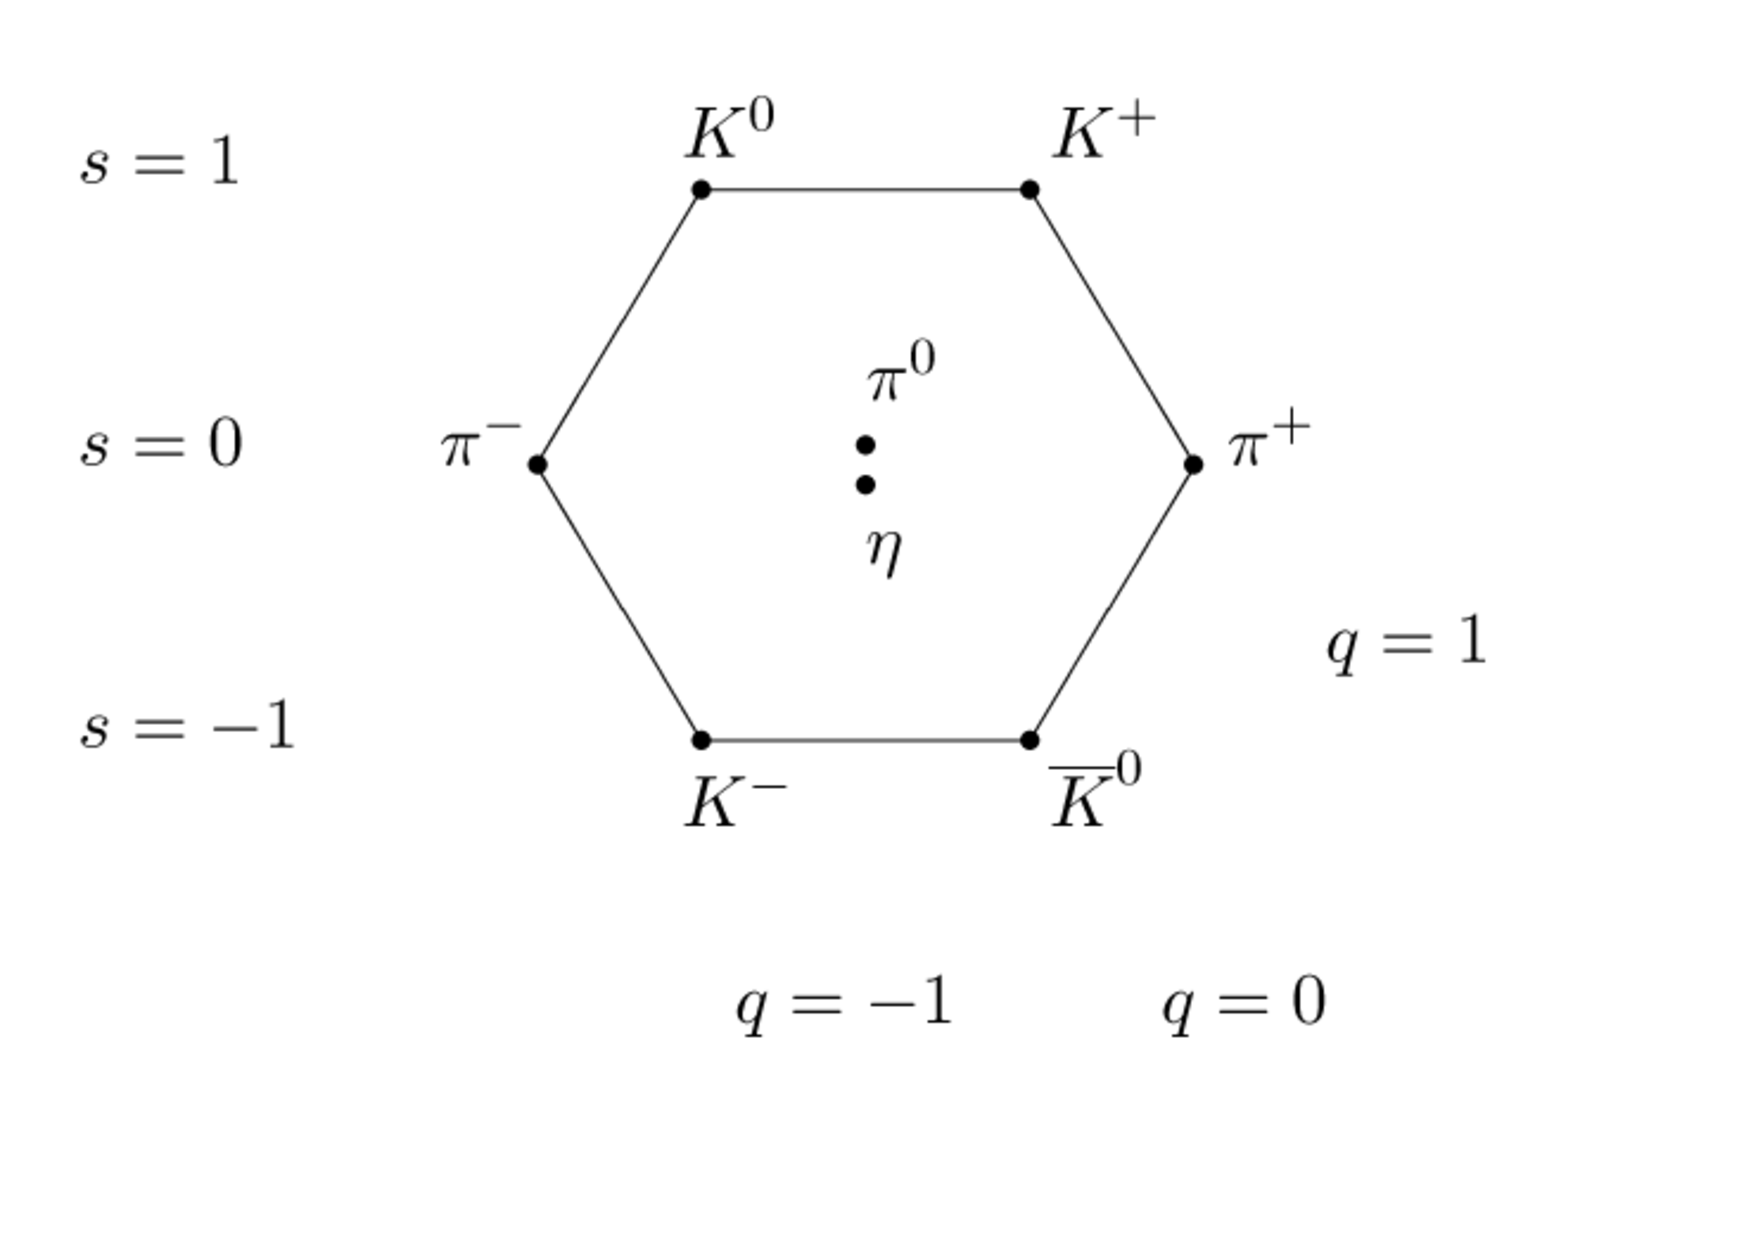
\includegraphics[width=0.7\textwidth]{imgs-MSc-thesis/ottuplice_via.pdf}
    \caption{QCD pseudoscalar meson octet in the Cartàn plane.}
    \label{fig:meson_octet}
\end{figure}
\newline
They form the pseudoscalar $J^P = 0^-$ meson octet - plus a singlet - of the QCD at low energies $\{ \pi^\pm,\pi^0,K^\pm,K^0,\bar K^0,\eta,\eta' \}$.
\textit{How} quarks are bound togheter is an unexplained question because it would need a formal non-perturbative development of QFT.
For this reason lattice QCD is a very powerful tool, allowing us to compute non-perturbative quantities through path integrals.
\newline
To give an example of confinement effects, let's consider a (non singlet flavour) pseudoscalar propagator - or two points functions - $G_{12}(x,y)$:
\begin{equation*}
    G_{12}(x,y) = \la 0 | T \left\{ ( \bar\psi^1 \gamma_5 \psi^2 )(x) ( \bar\psi^2 \gamma_5 \psi^1 )(y) \right\} | 0 \ra
\end{equation*}
for example, by choosing $\psi^1 = u$ and $\psi^2 = d$, the propagator of the $\pi^-$ si obtained.
In principle the two constituent quarks $\psi^1, \psi^2$ - named \textit{valence} quarks - are subject to a very large number of interactions with the gluons.
In first approximation of perturbation theory (PT) one simply neglects these contributions, while at higher orders only few diagrams are involved.
However the running coupling phenomenon makes the constant $g(\mu)_\text{colour}$ grow at energies below $\Lambda_\text{QCD}$. 
As a consequence the use of PT is no longer allowed and all the possible contributing diagrams must be considered.
The Figure \ref{fig:confinement} gives an idea of the subleading processes to involve.
\begin{figure}[h!]
    \centering
    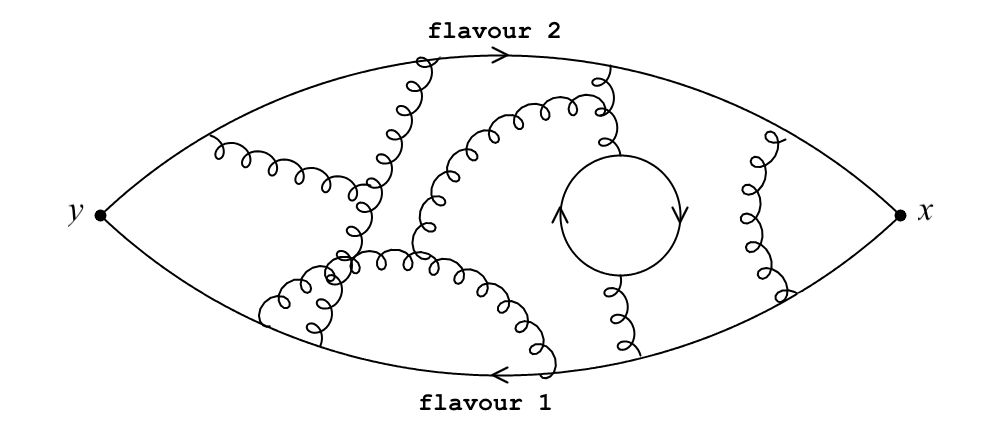
\includegraphics[width=0.9\textwidth]{imgs-MSc-thesis/confinement.png}
    \caption{Conceptual idea of non perturbative contributions to the correlator $G_{12}(x,y)$.}
    \label{fig:confinement}
\end{figure}
\newline
As can be seen from Figure \ref{fig:confinement}, some internal quark loops could arise.
These virtual quarks are named {\it sea} quarks and could differ from the valence quarks.
For example, at some point a pion could contain a couple of charm quarks $c\bar c$ without any apparent reason: they are virtual sea quarks.
By an appropriate scattering process, they could be even put on shell and extracted.
The conceptual difference between valence and sea quarks will be widely used in this work.

\section{Kaon oscillations in the Standard Model and $B_K$}
\noindent
The \kkb system ($m_K = 497.611 \pm 0.013 \mev$) is the doublet containing neutral $|s| = 1$ particles of the $0^-$ octet.
Because of decay channels of the Kaons in $2\pi, 3\pi$ and others \cite{ParticleDataGroup}, this is an \textit{open} system - in quantum mechanical sense.
For future use, I define two local operators:
\begin{equation}\label{eq:kkbar-operators}
    \begin{aligned}
        & K^0 & \text{neutral Kaon \space \space} \\
        & \bar K^0 & \text{neutral anti-Kaon}
    \end{aligned}
\end{equation}
which interpolate $| K^0\ra$ and $|\bar K^0\ra$ states.
In principle the two neutral Kaons are two different eigenstates of an effective Hamiltonian $H_0$;
thus we can choose a basis in which $H_0$ has the diagonal form:
\begin{equation*}
    H_0 =
    \begin{pmatrix}
        M - \frac{i}{2}\Gamma & 0 \\
        0 & M - \frac{i}{2}\Gamma
    \end{pmatrix}
    \qquad | K^0 \ra = 
    \begin{vmatrix}
        \hspace*{0.5mm} 1 \hspace*{0.5mm} \\ \hspace*{0.5mm} 0 \hspace*{0.5mm}
    \end{vmatrix}
    \qquad | \bar K^0 \ra = 
    \begin{vmatrix}
        \hspace*{0.5mm} 0 \hspace*{0.5mm} \\ \hspace*{0.5mm} 1 \hspace*{0.5mm}
    \end{vmatrix}
\end{equation*}
where $\Gamma$ gives the decay width.
This $H_0$ is associated the effective Schrodinger-like dynamics of the system:
\begin{equation*}
    i\frac{d}{d t} | \psi (t) \ra = H_0 | \psi (t) \ra
\end{equation*}
It is known that weak interactions add the following term to the Lagrangian density:
\begin{equation}
    \mathcal{L}_{\text{weak}} = \frac{g_2}{\sqrt{2}} \left[ \overline \psi^L_f \gamma_\mu W^{+}_\mu (V_{\text{CKM}})_{ff'} \psi^L_{f'} + \text{h.c.} \right]
\end{equation}
where $L$ stands for left component of the Dirac spinor, $V_{\text{CKM}}$ is responsible for flavour mixing, $f,f'$ are flavour family indices and $g_2$ is the weak coupling constant.
From the previous term this mixing 1-loop diagram follows:
\begin{center}
    \begin{tikzpicture}
        \centering
        \begin{feynman}
            \vertex (a1) {\(d\)};
            \vertex[right=2cm of a1] (a2);
            \vertex[right=2cm of a2] (a3);
            \vertex[right=2cm of a3] (a4) {\(s\)};

            \vertex[below=1.8cm of a1] (b1) {\(\overline s\)};
            \vertex[right=2cm of b1] (b2);
            \vertex[right=2cm of b2] (b3);
            \vertex[right=2cm of b3] (b4) {\(\overline d\)};

            \diagram* {
                {[edges=fermion]
                  (a1) -- (a2) -- [edge label=\({u,c,t}\)] (a3) -- (a4),
                  (b4) -- (b3) -- [edge label=\({\overline u, \overline c, \overline t}\)] (b2) -- (b1),
                },
                (a2) -- [boson, edge label=\(W\)] (b2),
                (a3) -- [boson, edge label'=\(W\)] (b3),
            };
        
            \draw [decoration={brace}, decorate] (b1.south west) -- (a1.north west)
                  node [pos=0.5, left] {\(K^{0}\)};
            \draw [decoration={brace}, decorate] (a4.north east) -- (b4.south east)
                node [pos=0.5, right] {\(\overline K^{0}\)};
        \end{feynman}
    \end{tikzpicture}
\end{center}
Weak interactions also generate another 1-loop channel and diagrams in higher orders of perturbation theory.
Because of the mixing process, the effective Hamiltonian of the \kkb system needs non-diagonal terms parametrized in $H^{\Delta S = 2}$.
A formal development can be found in \cite{Donoghue} and a new diagonal basis is built: the new Kaon states that diagonalize $H_0 + H^{\Delta S = 2}$ are $K_{L}$ and $K_{S}$ - named $K$ long and $K$ short.
Through CP symmetry arguments it comes out that, by considering only SM interactions, the allowed decays are $K_L \rightarrow 3\pi$ and $K_S \rightarrow 2\pi$.
Through measures of these decays one can extract some pseudo-observables and parametrize the amout of CP violation in the Standard Model.
In particular, phenomenologists uses the so called $\epsilon$ parameter \cite{Donoghue}.
In order to quantify the mixing and extract the abovementioned quantities, the mixing amplitudes are needed.
Below I will give some arguments needed to define {\it bag parameters}, strictly related to mixing amplitudes.
\newline
At low energies ($E \ll M_W \simeq 80 \gev$) the $W$ propagator can be replaced by $1/M_W^2$ and the effective Fermi interaction can be ruled out.
It consists in a pointlike interaction of four fermions, the coupling constant is the Fermi constant $G_F/\sqrt{2}$ and it links togheter two quarks in the up sector of $SU(2)_L$ with two quarks in the down sector:
\begin{equation}\label{eq:Fermi-interaction}
    \mathcal{L}_F = \frac{G_F}{\sqrt{2}} V_{u_1 d_1} V_{u_2 d_2}^* \Big[\bar u_1 \gamma_\mu (1-\gamma_5)d_1\Big] \Big[\bar d_2 \gamma_\mu (1-\gamma_5)u_2\Big] + \text{ similars}
\end{equation}
that's a product of currents + flavour mixing.\footnote{In the notation adopted, the left and right Dirac projectors have these definitions: $P_L = (1-\gamma_5)/2$, $P_R = (1+\gamma_5)/2$. Infos about the notation are in Appendix \ref{app:notations}.} 
The original Fermi interaction involves only two families of quarks and the $V_{\text{CKM}}$ matrix is replaced by the Cabibbo angle rotation matrix.
Through this Lagrangian one can build two \textit{candy} diagrams for Kaons oscillations.
By a direct calculation of these diagrams:
\begin{itemize}
    \item [$\triangleright$] a loop factor $1/(16\pi^2)$ appears;
    \item [$\triangleright$] there is a sum over the up-components intermediate-flavours: $$\sum_{i,j=u,c,t} V_{id} V_{is}^* V_{jd} V_{js}^*$$ useful to test the unitarity of $V_\text{CKM}$ matrix;
    \item [$\triangleright$] an effective operator $\Theta_1 = \left[\bar s \gamma_\mu (1+\gamma_5) d\right] \cdot \left[ \bar s \gamma_\mu (1+\gamma_5) d \right]$ arises.
\end{itemize}
The sum of the two diagrams gives:
\begin{equation*}
    \mathcal{A} + \mathcal{A}' \propto \left(\frac{G_F}{\sqrt{2}}\right)^2 \frac{2}{16\pi^2} \left[\sum_{i,j} V_{id} V_{is}^* V_{jd} V_{js}^*\right] \la \bar K^0 | \Theta_1 | K^0 \ra
\end{equation*}
In this evaluation, only 1-loop is considered.
\newline
I will now proceed to highlight a problem that is responsible for the lattice calculation done in this thesis work.
The oscillation effect is well understood in perturbation theory by the previous argument, but at low energies it is not sufficient to well describe the complete amplitude.
Confinement and running coupling generate bound states of quarks and an infinte number of gluon-quark and gluon-gluon interactions take place.
These interactions must be involved in a non perturbative calculation of the amplitude.
To parametrize them, we introduce a form factor named $B_K$ parameter.
For the same reason some form factors (or decay constants) $f_{\pi,K,\dots}$ appear in the PCAC relations.
\newline
Then the $B_K$ parameter clearly depends on the renormalization scale $\mu$ and parametrizes the deviation from the Vacuum Insertion Approximation (VIA) \cite{BKetmcollaboration}:
\begin{equation}\label{eq:B_K-definition}
    \la \bar K^0 | \Theta_1^\text{ren} (\mu) | K^0 \ra_\text{non pert.} = B_K(\mu) \la \bar K^0 | \hat\Theta_1 | K^0 \ra_\text{VIA} = \frac{8}{3} m_K^2 f_K^2 B_K(\mu)
\end{equation}
Sometimes I will refer to $B_K$ as $B_1$ and to $\Theta_1^\text{ren} (\mu)$ as $\hat\Theta_1$.
The entire process in the Standard Model is graphically represented - in momentum space - by:
\begin{figure}[!h]
    \centering
    \begin{tikzpicture}
      \begin{feynman}
        \vertex[blob] (m) at ( 0, 0) {\contour{white}{$\Theta_1$}};
        \vertex (a) at (-3,-1) {$\overline s$};
        \vertex (b) at ( 3,-1) {$\overline d$};
        \vertex (c) at (-3, 1) {$d$};
        \vertex (d) at ( 3, 1) {$s$};
        \diagram* {
          (c) -- [fermion] (m) -- [fermion] (a),
          (b) -- [fermion] (m) -- [fermion] (d),
        };
        \draw [decoration={brace}, decorate] (a.south west) -- (c.north west)
        node [pos=0.5, left] {\(K^{0}\)};
        \draw [decoration={brace}, decorate] (d.north east) -- (b.south east)
        node [pos=0.5, right] {\(\overline K^{0}\)};
        \end{feynman}
    \end{tikzpicture}
\end{figure}
\newline
The value of $B_K$ is assessed non perturbatively by the ETM (Europen Twisted Mass) collaboration and it is reported by the FLAG working group in \cite{FLAG}\cite{ParticleDataGroup}:
\begin{equation}\label{B_K-value}
    B_K^{\overline{MS}}(2 \gev) = 0.524(13)(12)    
\end{equation}
Renormalization constants have been evaluated too.

\section{BSM effects: new operators and $B_i$ parameters}
\noindent
There exists a set of theories beyond the Standard Model (BSM) that give contributions to the \kkb oscillations - supersymmetry, multi-Higgs models, etc.
For this reason it is useful to study other operators $\{\Theta_i,\tilde\Theta_j\}$ - similar to $\Theta_1$ - that cause the mixing BSM.
They are used to define an effective Hamiltonian for the mixing process:
\begin{equation*}
    \mathcal{H}_\text{eff} = \frac{1}{4} \sum_{i = 1}^5 C_i \Theta_i + \frac{1}{4} \sum_{i = 1}^3 \tilde C_i \tilde \Theta_i
\end{equation*}
The operators $\{\Theta_i,\tilde\Theta_j\}$ have dimension 6 and are composed by four quark fields, while $\{C_i,\tilde C_j\}$ are their Wilson coefficient.
They arise at low energies in a way similar to $\Theta_1$, presented in the previous section.
One common choice for the basis of these operators is the so called \textit{SUSY basis} \cite{Bparameters}, used in BSM phenomenology:
\begin{equation}\label{eq:Thetai-operators}
    \begin{aligned}
       & \Theta_1 = [\bar s^a \gamma_\mu (1-\gamma_5) d^a] \cdot [ \bar s^b \gamma_\mu (1-\gamma_5) d^b ] \\
       & \Theta_2 = [\bar s^a  (1-\gamma_5) d^a ] \cdot [ \bar s^b (1-\gamma_5) d^b ] \\
       & \Theta_3 = [\bar s^a  (1-\gamma_5) d^b ] \cdot [ \bar s^b (1-\gamma_5) d^a ] \\
       & \Theta_4 = [\bar s^a  (1-\gamma_5) d^a ] \cdot [ \bar s^b (1+\gamma_5) d^b ] \\
       & \Theta_5 = [\bar s^a  (1-\gamma_5) d^b ] \cdot [ \bar s^b (1+\gamma_5) d^a ] \\
       & \tilde\Theta_1 = [\bar s^a \gamma_\mu (1+\gamma_5) d^a] \cdot [ \bar s^b \gamma_\mu (1+\gamma_5) d^b ] \\
       & \tilde\Theta_2 = [\bar s^a  (1+\gamma_5) d^a] \cdot [ \bar s^b (1+\gamma_5) d^b ] \\
       & \tilde\Theta_3 = [\bar s^a  (1+\gamma_5) d^b] \cdot [ \bar s^b (1+\gamma_5) d^a ]
    \end{aligned}
\end{equation}
where $a,b$ are colour indices\footnote{Einstein summation convention is used.} and within the square brackets $[\hspace*{0.5mm}\cdot\hspace*{0.5mm}]$ a sum over spin is implied.
The first operator is the one of the Standard Model cited in the previous section.
I will study the bare matrix elements $\la \bar K^0 | \Theta_j | K^0 \ra$ in a lattice environment in which only strong interactions take place; it is known that strong interactions preserve both $\mathbb{C}$ and $\mathbb{P}$ symmetries, thus only the parity preserving part of these operators, denoted by $\Theta_i^{[+]}$ will be considered \cite{KMBSM}.
In the case of $\Theta_j$ and $\tilde\Theta_j$ the parity even parts are the same, then only 5 even operators are needed.
A more detailed discussion about these operators and their lattice counterparts is presented in Chapter \ref{ch:operators}.

\subsection{Bag parameters}
\noindent
The bag parameters $B_i(\mu)$s arise through the same confinement argument concerning $B_K$ and a scaling behaviour with $\mu$ is naturally expected.
$B_i(\mu)$s are defined by the following equations \cite{Bparameters}:
\begin{equation*}
    \begin{aligned}
        & \la \bar K^0 | \Theta_1^{[+],\ren}(\mu) | K^0 \ra = \frac{8}{3} m_K^2 f_K^2 B_1(\mu) \\
        & \la \bar K^0 | \Theta_2^{[+],\ren}(\mu) | K^0 \ra = -\frac{5}{3} \left(\frac{m_K}{m_s(\mu)+m_d(\mu)}\right)^2 m_K^2 f_K^2 B_2(\mu) \\
        & \la \bar K^0 | \Theta_3^{[+],\ren}(\mu) | K^0 \ra = \frac{1}{3} \left(\frac{m_K}{m_s(\mu)+m_d(\mu)}\right)^2 m_K^2 f_K^2 B_3(\mu) \\
        & \la \bar K^0 | \Theta_4^{[+],\ren}(\mu) | K^0 \ra = 2 \left(\frac{m_K}{m_s(\mu)+m_d(\mu)}\right)^2 m_K^2 f_K^2 B_3(\mu) \\
        & \la \bar K^0 | \Theta_5^{[+],\ren}(\mu) | K^0 \ra = \frac{2}{3} \left(\frac{m_K}{m_s(\mu)+m_d(\mu)}\right)^2 m_K^2 f_K^2 B_3(\mu)
    \end{aligned}
\end{equation*}
with $m_d (\mu)$ and $m_s (\mu)$ the renormalized masses of quarks down and strange in the same renormalization scheme applied for $\Theta_i^{[+],\ren}(\mu)$.
The previous equations can be rewritten in a more compact way, as in \cite{KMBSM}:
\begin{equation}\label{eq:bag-definition}
    \begin{aligned}
        & \la \bar K^0 | \Theta_1^{[+],\ren}(\mu) | K^0 \ra = \xi_1 m_K^2 f_K^2 B_1(\mu) \\
        & \la \bar K^0 | \Theta_j^{[+],\ren}(\mu) | K^0 \ra = \xi_j \left(\frac{m_K^2}{m_s(\mu)+m_d(\mu)}\right)^2 f_K^2 B_j(\mu) \quad \quad \text{ for } j=2,\dots,5
    \end{aligned}
\end{equation}
with $\xi_i = \left(8/3, -5/3, 1/3, 2, 2/3\right)$ numerical factors.
The definitions of bare Bag parameters are analogous to the above mentioned but involve only bare quantities.
The numerical value of $B_i$-parameters is extracted in \cite{Bparameters} and a large amount of other papers.
A relevant work has been done by the ETM collaboration in \cite{KMBSM} bringing these results at $\mu_0 = 2\gev$ in the $\overline{MS}$ scheme:
\begin{equation}\label{eq:b_i-in-kmbsm}
    \begin{aligned}
        & B_1(\mu_0) = 0.53(2) \quad B_2(\mu_0) = 0.52(2) \quad B_3(\mu_0) = 0.89(5) \\
        & \hspace*{18mm} B_4(\mu_0) = 0.78(3) \quad B_5(\mu_0) = 0.57(4)
    \end{aligned}
\end{equation}
I want to highlight that the $B_1(\mu_0)$ value has a small difference with respect to the one in formula \ref{B_K-value} - because it comes from a different simulation - but fortunately there is an overlap due to statistical errors.
The simulation setup developed in this thesis is very similar to the one used in \cite{KMBSM}, but some improvements have been done.
Such improvements are discussed in the next chapters.
Some simulation results at the scale of $\mu=3$\gev\space are reported in the second graph in Figure \ref{fig:bag-parameters}.
\begin{figure}[h!]
    \centering
    \begin{subfigure}[b]{0.49\textwidth}
        \centering
        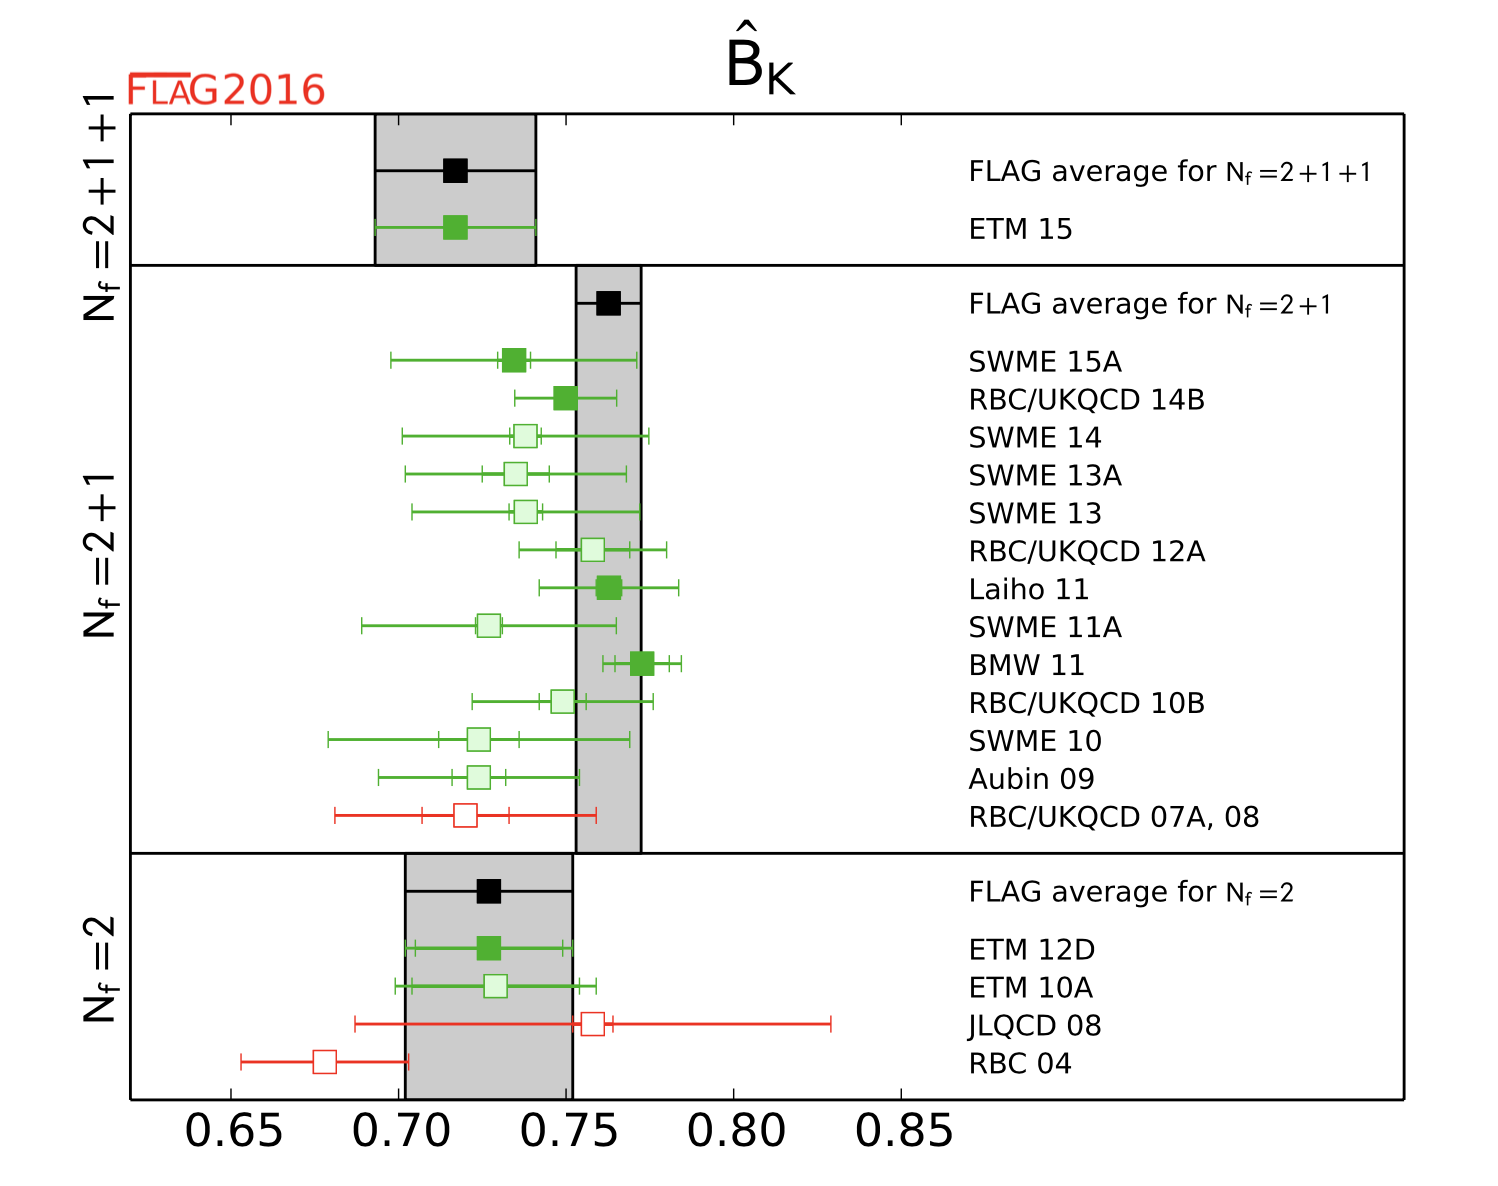
\includegraphics[width=\textwidth]{imgs-MSc-thesis/flag-Bk.png}
        \caption{$\hat B_K$}
    \end{subfigure}
    \begin{subfigure}[b]{0.49\textwidth}
        \centering
        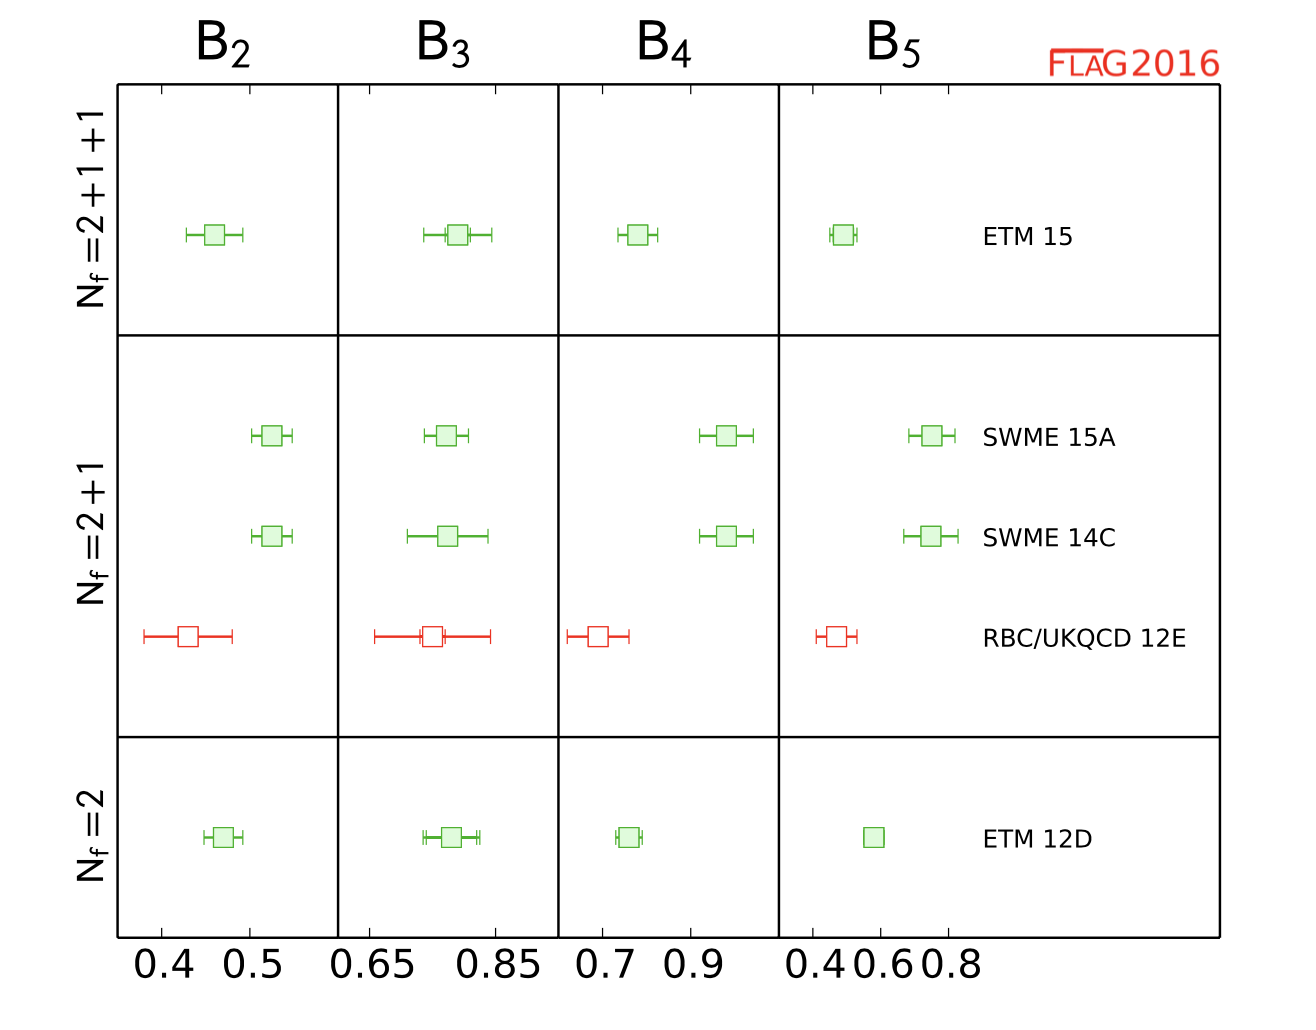
\includegraphics[width=\textwidth]{imgs-MSc-thesis/flag-Bi.png}
        \caption{$B_i^{\overline{MS}} (\mu = 3 \text{ Gev})$}
    \end{subfigure}
    \caption{Current lattice results until 2016, July 1st, date of pubblication of the report by FLAG Working Group \cite{FLAG}.
        Figure (a): lattice results of the renormalization group invariant $\hat B_K$ from distinct simulations.
        Figure (b): lattice results of the renormalized bag parameters with index $i = 2,3,4,5$ in the $\overline{MS}$ scheme at energy scale of 3\gev.}
    \label{fig:bag-parameters}
\end{figure}
\newline
The first graph refers to $\hat B_K$, a renormalization group invariant for the $B_K$ parameter defined by \cite{FLAG}:
\begin{equation*}
    \hat B_K = \left(\frac{\overline{g}(\mu)^2}{4 \pi}\right)^{-\gamma_0/(2\beta_0)}\times \text{exp}\left\{ \int_0^{\overline{g}(\mu)} dg \hspace*{.5mm} \left( \frac{\gamma (g)}{\beta (g)} + \frac{\gamma_0}{\beta_0 g}\right) \right\} B_K (\mu)
\end{equation*}
\newline
The results (\ref{eq:b_i-in-kmbsm}) should be compared with the new values estimated through the program of this work.
This comparison needs a renormalization of mixing operators (\ref{eq:Thetai-operators}) not involved is this thesis program.

%%%%%%%%%%%%%%%%%%%%%%%%%%%%%%%%%%%%%%%%%%%%%%%%%%%%%%%%%%%%%%%%%%%%%%%%%%%%%%%%%%%%%%%%%
%%%%%%%%%%%%%%%%%%%%%%%%%%%%%%%%%%%% SECOND CHAPTER %%%%%%%%%%%%%%%%%%%%%%%%%%%%%%%%%%%%%
%%%%%%%%%%%%%%%%%%%%%%%%%%%%%%%%%%%%%%%%%%%%%%%%%%%%%%%%%%%%%%%%%%%%%%%%%%%%%%%%%%%%%%%%%
\chapter{Lattice regularization and improvements}\label{ch:lattice-regularization}
\lettrine[lines=2, findent=3pt, nindent=0pt]{T}{}he purpose of this chapter is to introduce the reader to the fundamentals of lattice regularization and to detail the specific approach adopted in this study.
\newline
In order to calculate Kaon matrix elements, a non perturbative approach is required and the path integral formulation provides for this \cite{Itzykson-Zuber}.
As known, a path integral involves an \textit{infinite} sum of field configurations defined on an \textit{infinite} volume and time extension.
Despite this, vacuum expectation values of physical observables yield to \textit{finite} quantities.
A well defined simualtion needs a regularization that faces the problem of these infinites.
For this reason lattice QFT is a very useful regularization.
It involves discretizing spacetime, referred to as the lattice, along with a finiteness of the volume.
The two most relevant sources of errors are the discretization of the space and the finite volume effects.
To deal with these errors, a large number of improvements has been developed through the years and some of them find application in this work.
\newline
The first section will provide a general overview of lattice regularization of a quantum field theory.
In the second and third sections I will discuss respectively gauge and fermion fields regularizations on the lattice;
I will start from the simplest regularizations and I will progressively extend them to the improved ones, which are used.
In the fourth section, a specific set of bosonic ghost fields will be described.
The fifth section will delineate the lattice regularization employed in the present simulation.
Finally, the sixth section provides an overview about the \obc, which represent one of the two peculiarities of this work compared to those previously carried out.

\section{Lattice regularization of QFT}\label{sec:lattice-discretization}
\noindent
A finite and discretized functional integral can be formulated by implementing the following modifications to the continuous functional integral \cite{montvay-munster}\cite{gattringer-lang}:
\begin{itemize}
    \item [$\triangleright$] The Minkowski space $\mathbb{M}^4$ is replaced with an hypercubic lattice of $N_\text{time} \times N_\text{space}^3$ points.
        The volume $V$ and time extension $T$ become finite quantities and the separation between two adjacent lattice points takes the name of \textit{lattice spacing} $a$.
        Therefore, the lattice space is defined as:
        \begin{equation*}
            \Lambda = \{x = a\cdot(n_1,n_2,n_3,n_4) | n_{1,2,3} = 0,\dots,N_\text{space}-1 \text{ and } n_4 = 0,\dots,N_\text{time}-1 \}
        \end{equation*}
        Clearly the physical extension of the lattice is given by $a\cdot(N_\text{time},N_\text{space}^3) = (T,L\times L\times L)$.
        Continous spacetime symmetries - e.g. rotations - are now replaced by hypercubic symmetries on the lattice.
    \item [$\triangleright$] Consider a set of quantum fields $\tilde\phi_i(x), i = 1,\dots, N_\text{fields}$ in the continuum theory.
        In lattice path integral formulation they are treated as smooth local functions defined on $\Lambda$:
        \begin{equation*}
            \begin{aligned}
                \phi_i : \hspace*{3mm}
                & \Lambda \longrightarrow \mathbb{R}, \mathbb{C}, SU(N_C), \dots \\
                & x \longmapsto \phi_i (x)
            \end{aligned}
        \end{equation*}
    \item [$\triangleright$] The continuum action of the fields $S^\text{cont}[\tilde\phi_1,\dots,\tilde\phi_{N_\text{fields}}]$ must be discretized - i.e. replace the derivatives with discrete derivatives and, eventually, add some terms.\footnote{The additive terms must vanish in the continuum limit}
        The fundamental requirement is that the lattice action has the right continuum limit: $$S^\text{Lat}[a;\phi_1,\dots,\phi_{N_\text{fields}}] \xrightarrow{\hspace*{3mm} a \rightarrow 0\hspace*{3mm}} S^\text{cont}[\tilde\phi_1,\dots,\tilde\phi_{N_\text{fields}}]$$
    \item [$\triangleright$] The integration measure of the path integral takes the following form:
        \begin{equation*}
            \mathcal{D}\tilde{\phi} \longmapsto \prod_{i=1}^{N_\text{fields}} \prod_{x\in \Lambda} d\phi_i (x)
        \end{equation*}
        For notational convenience the measure is again denoted by $\mathcal{D}\phi$.
\end{itemize}
These changes together constitute the \textit{lattice regularization} of a continuum theory. 
Sometimes I will use the word ``regularization'' to refer to the action discretization, that's the only non trivial part of a lattice regularization procedure. 
\newline
As usual in continuum path integral, given an observable $\mathcal{X}$ functional of the fields, its expectation value on the vacuum is given by:
\begin{equation*}
    \la \mathcal{X} (x_1,\dots,x_K) \ra = \frac{1}{\mathcal Z} \int \mathcal{D} \phi \hspace*{0.5mm} e^{-S_E[\phi_i]} \mathcal{X}\left[\phi_1,\dots,\phi_{N_\text{fields}}\right] (x_1,\dots,x_K)
\end{equation*}
where $\mathcal Z$ is the usual partition function $\mathcal Z = \la 1 \ra$.
The path integral provides theoretical tools to handle a non perturbative theory then all the quantities in lattice simulations must be evaluated through vacuum expectation values of some chosen observables \cite{Itzykson-Zuber}.
This fact has consequences, for example the asymptotic extractions described in section \ref{sec:asympt-behav}.
\newline
In the case of QCD described in the previous chapter, the integration can be split in two parts: the {\it fermionic integration} $\la \hspace*{0.7mm} \cdot \hspace*{0.7mm} \ra_F$ with measure $\mathcal{D}\psi\mathcal{D}\bar\psi$ and the {\it Gauge integration} $\la \hspace*{0.7mm} \cdot \hspace*{0.7mm} \ra_G$ with measure $\mathcal{D}U$ \footnote{About the meaning of the variables $U_\mu$, wait until the next section.}.
Since it is impossible to numerically simulate Grassman variables, the fermionic integral requires a theoretical calculation while the simulation allows us to evaluate the Gauge integral:
\begin{equation*}
    \left\la \mathcal{X} \right\ra = \left\la \left\la \mathcal{X} \right\ra_F^\text{th.} \right\ra_G^\text{sim.}
\end{equation*}
This is a fundamental step for the lattice simulations.
If $\mathcal{X}$ is a polynomial on the fermion fields, Wick theorem applies\footnote{Wick theorem holds only in case of bilinear actions: $$S_F[\psi,\bar\psi ,U] = \sum_{x,y}\bar \psi (x) D[U](x,y) \psi (y)$$ } and a {\it fermion determinant} $\text{det}\left(D[U]\right)$ appears in the functional integral:
\begin{equation}\label{eq:fermion-determinant}
    \begin{aligned}
        \la \mathcal{X} \ra
        & = \frac{1}{\mathcal Z} \int \mathcal{D}U \mathcal{D}\psi \mathcal{D}\bar\psi \hspace*{0.5mm} e^{-S_G[U]-S_F[\psi,\bar\psi ,U]} \hspace*{0.5mm} \times \hspace*{0.5mm} \mathcal{X} [\psi,\bar\psi] = \\
        & = \frac{1}{\mathcal Z} \int \mathcal{D}U \hspace*{0.5mm} e^{-S_G[U]} \text{det}\left(D[U]\right) \hspace*{0.5mm} \times \hspace*{0.5mm} \text{Wick terms}[U] = \\
        & = \frac{1}{\mathcal Z} \int \mathcal{D}U \hspace*{0.5mm} e^{-S_G[U] + \tr \ln D[U]} \hspace*{0.5mm} \times \hspace*{0.5mm} \text{Wick terms}[U]
    \end{aligned}
\end{equation}
Sometimes the exponentiated term $S_\text{eff}[U] = S_G[U] - \tr \ln D[U]$ is called {\it effective Gauge action}.
Equation (\ref{eq:fermion-determinant}) and the concept of fermion determinant will be useful in the next sections.
A good question is about the role of fermion determinant in the functional integral.
It contains the interaction terms between Gauge fields $U$ and fermions, so it introduces the fermion virtual loops in the correlation functions.
In other words, the distinction between effective Gauge action and the standard action $S_G[U]$ resides in the presence of quark loops contributions.
This can be easily checked in perturbation theory.
For this reason, only {\it sea} quarks need a fermion determinant, while {\it valence} quarks are inserted only as external fermions.
Is it noteworthy the existence of an approximation - not used in this work - called ``quenched approximation'' in which the fermion determinant is neglected.
This approximation corresponds to the neglection of sea quarks loops.
To better understand the sea vs valence concept the following image could be useful.
\begin{figure}[h!]
    \centering
    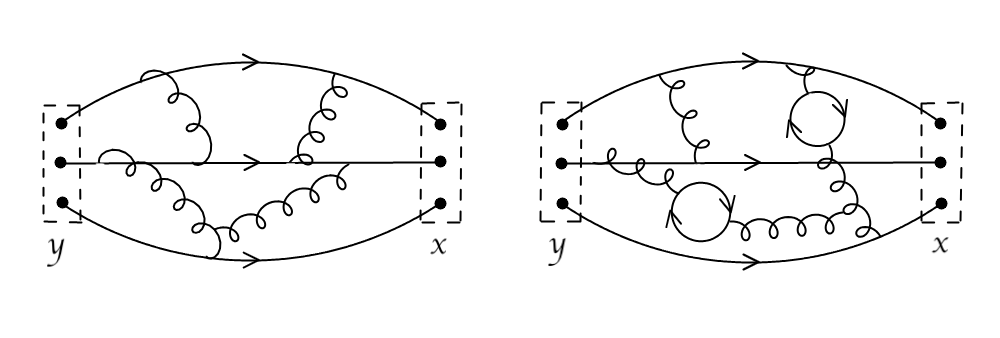
\includegraphics[width=0.9\textwidth]{imgs-MSc-thesis/quenched.png}
    \caption{One the right: a complete baryon propagator $G_B(x,y) = \la B(x) B^\dagger (y) \ra$.
        On the left: the same propagator in quenched approximation.
        In non-perturbative QCD, most of the times gluon propagators are not drawn, because they are infinite in number.
        For this reason next graphs will not include them.}
    \label{fig:quenched-approximation}
\end{figure}
\newline
The general strategy to evaluate correlators like $\la\mathcal{X}\ra$ follows.
First, the correlator must be calculated at different values of lattice spacing $\la\mathcal{X}\ra |_a$.
Then a {\it continuum limit} of $\la\mathcal{X}\ra \equiv \la\mathcal{X}\ra |_0$ can be extracted for $a \rightarrow 0$.
Since physics resides in the continuum limit, there is a sort of \textit{residual freedom} in the choice of the regularization.
All the valid regularizations share the same physical continuum limit, differing only by $O(a^n)$ terms, with $n\ge 1$.
Clearly these terms are nothing but lattice artifacts that don't give contributions to the exact continuum limit and don't have any physical meaning.
However the continuum limit is approached by extrapolation, then actions that contains only $O(a^2)$ lattice terms or higher give more precise values than actions with $O(a)$ terms.
These regularized actions are called {\it \oaid \space actions} and some of them are described below.
Moreover, an \oaid \space action can always be obtained from an $O(1)-$action by adding some counterterms that cancel the $O(a)$ lattice artifacts.
In some cases, an \oaid\space action guarantees an $O(a)-$improvement only for a particular set of observables;
for example a symmetry conservation could cause an \oait\space on some observables that have a definite quantum number under the given symmetry.

\section{Gauge action}
\noindent
The first proposal to regularize Gauge and fermion action on the lattice was advanced by Wilson in 1974 \cite{Wilson-Confinement-of-Quarks}.
Usually Gauge fields are denoted by $A_\mu (x) \equiv A_\mu^a(x)T^a_{\square}$ and the continuum action is defined in formula (\ref{eq:masslessQCD}).
An alternative way to introduce Gauge fields is to treat them as connections, by defining a Wilson line $W(x,y)$ \cite{Schwartz}.
This formulation is useful in this case because the steps towards lattice theory are very simple and natural.
A Wilson line is defined by:
\begin{equation*}
    W(x,y) = P \left\{\text{exp}\left(i\int_y^x A_\mu(\omega)d\omega^\mu\right)\right\}
\end{equation*}
with $P$ denoting the path ordering product.
It is proven that a Wilson line transforms in this way under Gauge transformations $\mathcal{U}\in SU(N)$:
\begin{equation}\label{eq:wline-transformation}
    W(x,y) \longmapsto \mathcal{U}(x) W(x,y) \mathcal{U}(y)^\dagger
\end{equation}
By choosing an integration path in direction $\hat\mu = (\delta_{\mu 1},\delta_{\mu 2},\delta_{\mu 3},\delta_{\mu 4})$ with length equal to the lattice spacing $a$, Wilson line is approximated by:
\begin{equation*}
    W_\mu(x+a\hat\mu, x) \approx \text{exp}\left(iaA_\mu (x)\right) := U_\mu (x)
\end{equation*}
The line $U_\mu$ is called a {\it link variable} and it will be useful to build a Gauge invariant fermion action in the next section.
It is represented as a line connecting a lattice point $x$ with the adjacent point in direction $\hat\mu$, i.e. $x+a\hat\mu$ (or simply $x+\hat\mu$).
\newline
To provide a regularized Gauge action, a Gauge invariant quantity must be built.
One simple way is to multiply four link variables in a way such that they link the initial point $x$ to itself.
\begin{equation*}
    U_P^{\mu\nu}(x) \equiv U_\mu (x) U_\nu (x+\hat\mu) U_{-\mu} (x+\hat\mu+\hat\nu) U_{-\nu} (x+\hat\nu)
\end{equation*}
This is called {\it plaquette} of link variables in the $\mu-\nu$ plane and it is shown in Figure \ref{fig:plaquette}.
\begin{figure}[h!]
    \centering
    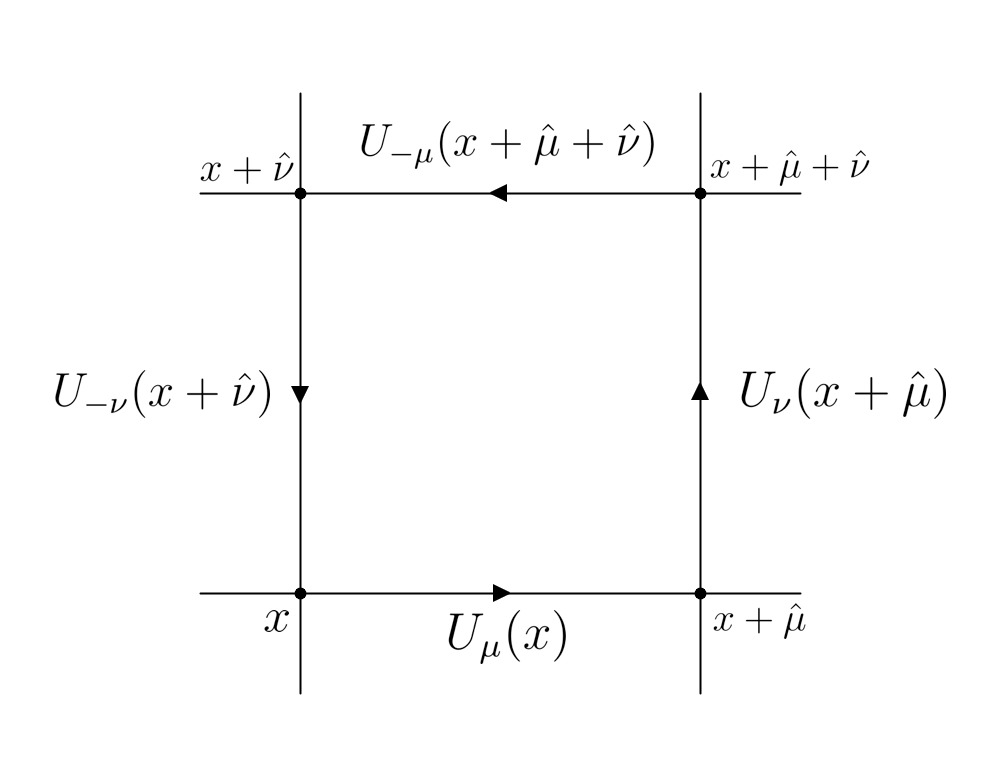
\includegraphics[width=0.75\textwidth]{imgs-MSc-thesis/plaquette.png}
    \caption{A plaquette in the $\mu-\nu$ plane, useful to build (\ref{eq:wgaugeaction})}
    \label{fig:plaquette}
\end{figure}
The trace of a plaquette is Gauge invariant and it is easy to prove by applying formula (\ref{eq:wline-transformation}) and cyclicity property of the trace.
Then the \textit{Wilson Gauge action} is built in the following way:
\begin{equation}\label{eq:wgaugeaction}
    S_G[U] = \frac{\beta}{3}\sum_{\{p\}} \tr \left[ \mathbb{I} - U(p)\right]
\end{equation}
where $\{p\}$ is the set of positively oriented plaquettes and $\beta = 6/g_0^2$ depends on the bare coupling $g_0$.
It can be proven that in the continuum limit this action corresponds to the dynamical part of Gauge action in formula (\ref{eq:masslessQCD}).
To do this, just apply BCH formula and the definition of the link variables \cite{gattringer-lang}.
By developing explicit calculations, it is clear that this action is not \oaid.
\newline
Several $O(a)-$improvements are available and some of them are expressed in the following way:
\begin{equation}\label{eq:gaugeaction-LuscherWeisz}
    S_G[U] = \frac{1}{g_0^2} \left\{ c_0 \sum_{\{p\}} \tr \left[ \mathbb{I} - U(p)\right] + c_1 \sum_{\{r\}} \tr \left[ \mathbb{I} - U(r)\right] \right\}
\end{equation}
where $\{r\}$ is a set of rectangles on the lattice, analogous to $\{p\}$.
Depending on the choice of the coefficients $c_{0}$ and $c_{1}$, it is possible to get different improvements.
The chosen one uses $c_0 = 5/3$ and $c_1 = -1/12$ and takes the name of \textit{Luscher-Weisz action} \cite{tmLQCD}.

\section{Fermion actions}\label{sec:fermion-discretization}
\noindent
A large number of different regularizations of fermions are available at current times.
In this wide section I will describe some of them that differ from each other by improvements and other features.
A shortlist of the regularizations described could be useful to clarify the general purpose, that's to give to the reader all the needed tools to understand the adopted regularization of the work (see section \ref{sec:setup}):
\begin{itemize}
    \item [$\triangleright$] In \ref{subsec:naive-wd-action} I will introduce the basic actions of lattice QCD: the \textit{Naive action} and the \textit{Wilson-Dirac action}.
        They serve as a background to build other cutting edge actions.
    \item [$\triangleright$] In \ref{subsec:SWterm} I will describe the Sheikholeslami-Wohlert term.
        It is a term to be addded to Wilson-Dirac fermion action to get the \oait\space of the theory.
        It will also be useful for other reasons explained at the end of the chapter.
    \item [$\triangleright$] The subsection \ref{subsec:zero-modes} will describe the problem of zero modes related to the Wilson Dirac action.
        Moreover it introduces the issue of explicit chiral symmetry breaking on the lattice.
    \item [$\triangleright$] The \textit{twisted mass QCD} (tmQCD) and \textit{Maximally twisted mass QCD} (MtmQCD), described in \ref{sec:tmLQCD}, are introduced to solve the problem of zero-modes.
        MtmQCD is a special case of tmQCD. Moreover MtmQCD has the property to be an \oaid\space action.
    \item [$\triangleright$] Despite the powerful properties of tmQCD, it is not used in this work\footnote{In section \ref{sec:obc} it will be clear how the tmQCD is not necessary: its properties are achieved in other ways.} but it is replaced by the \textit{Osterwalder-Seiler action}, very similar to it.
        In some particular cases OS action \textit{coincides} with tmQCD.
        This regularization is described in \ref{sec:OS-regularization}.
    \item [$\triangleright$] In section \ref{sec:ghosts} I introduce some bosonic ghost fields needed to well simulate valence quarks.
\end{itemize}


\subsection{Wilson-Dirac action}\label{subsec:naive-wd-action}
\noindent
The continuum fermion euclidean lagrangian density $\mathcal{L}_0^E = \bar \psi_q (x) \left( \gamma_\mu D_\mu + m \right) \psi_q (x)$ can be discretized by following the steps in section \ref{sec:lattice-discretization}.
In order to achieve Gauge invariance, a covariant derivative on the lattice is introduced.
The auxiliary Gauge fields take the form of link variables, i.e. Wilson lines.
The resulting action is called \textit{naive action} of fermions on the lattice \cite{montvay-munster}\cite{gattringer-lang}:
\begin{equation*}
    \begin{aligned}
        S [\psi,\bar \psi, U]
        & = a^4\sum_{q,x} \bar \psi_q (x) \left( \gamma_\mu \frac{U_\mu (x) \psi_q (x+\hat\mu) - U_{-\mu}(x)\psi_q(x-\hat\mu)}{2a} + m_q \psi_q (x) \right) = \\
        & = a^4\sum_{q,x} \bar \psi_q (x) \left( \frac{1}{2}\gamma_\mu (\nabla_\mu + \nabla^*_\mu) + m_q \right) \psi_q (x)  \\
    \end{aligned} 
\end{equation*}
where $q$ is the flavour index and a sum over $\mu$ is implied.
In the last line I've implicitly declared the discretized version of forward and backward covariant derivatives:
\begin{equation*}
    \begin{aligned}
        & \nabla_\mu \psi (x) = \frac{1}{a}\left[U_\mu (x) \psi (x+\hat\mu)-\psi (x)\right] \\
        & \nabla^*_\mu \psi (x) = \frac{1}{a}\left[\psi (x) - U_\mu (x-\hat\mu) \psi (x-\hat\mu)\right] \\
    \end{aligned}
\end{equation*}
It can be easily checked that the Gauge invariance of the action is achieved.
\begin{equation*}
    \text{Gauge transformations:} 
    \begin{cases}
        \psi (x) \mapsto \mathcal{U}(x) \psi (x) \\
        \bar\psi (x) \mapsto \bar\psi (x) \mathcal{U}(x)^\dagger \\
        U_\mu (x) \mapsto \mathcal{U} (x) U_\mu (x) \mathcal{U} (x+\hat\mu)^\dagger
    \end{cases}
\end{equation*}
for example $\bar \psi (x) \gamma_\mu U_\mu (x) \psi (x + \hat \mu) \mapsto \bar\psi (x) \mathcal{U}(x)^\dagger \mathcal{U} (x) \gamma_\mu U_\mu (x) \mathcal{U} (x+\hat\mu)^\dagger \mathcal{U}(x+\hat\mu) \psi (x)$ is invariant;
the same holds for the other terms.
\newline
In the free case ($U_\mu (x) = \mathbb{I}_3 \hspace*{1mm} \forall \mu ,x$) this action gives the right continuum fermion propagator for $a\rightarrow 0$, but the problem of \textit{fermion doubling} arises \cite{montvay-munster}:
by taking the discrete Fourier transform of the discretized free Dirac operator, it can be proved that its inverse has poles in $p_\mu = (0,0,0,0)$ and 15 many other non physical momenta - e.g. $p_\mu = (\pi/a,0,0,0), (0,\pi/a,0,0), (\pi/a,\pi/a,0,0),\dots$.
These non physical momenta are named \textit{doublers} and are suppressed through the insertion of an additive piece to the action:
\begin{equation}\label{eq:wilson-fermions}
    \begin{gathered}
        S[\psi,\bar \psi, U] = a^4\sum_{q,x,y} \bar \psi_q (x) \left( D^W_{xy}(r_q) + m_q \delta_{xy}  \right) \psi_q (y) \\
        \begin{aligned}
            D_{x,y}^W (r_q)
            & = -\frac{1}{2a}\sum_{\mu = \pm 1}^{\pm 4} \left[ (\mathbb{I}_4 \hspace*{0.5mm} r_q - \gamma_\mu)U_\mu (x) \delta_{x,y-\hat \mu} \right] + \frac{4r_q}{a}\delta_{xy} = \\
            & = \frac{1}{2}\left(\gamma_\mu(\nabla_\mu +\nabla_\mu^*) - a\hspace*{0.5mm}r_q\hspace*{0.5mm}\nabla_\mu^*\nabla_\mu\right)_{xy}
        \end{aligned}
    \end{gathered}
\end{equation}
where $\gamma_{-\mu} \equiv -\gamma_\mu$ and the Wilson parameters $r_q$ must satisfy $|r_q|\in(0,1]$ for each $q$.
Whenever the sum over $\mu$ is omitted, it is to be understood as a sum over $\mu = 1, \dots, 4$.
The usual choice for the parameter $r_q$ is 1, while the value $r_q = 0$ gives the naive action.
Action (\ref{eq:wilson-fermions}) is called \textit{Wilson-Dirac action} of fermions on the lattice and it is the most used fermion discretization on the lattice.
Because of the additive piece, the doublers gets an infinite mass for $a \rightarrow 0$, thus they tend to inexcitable modes of the theory.
In this simple way the doublers problem is solved.
The definition of this action is not equal to the one in \cite{montvay-munster}\cite{gattringer-lang} but equivalent.
At the current point, there are no $O(a)-$improvements.

\subsection{\oait: Sheikholeslami-Wohlert term}\label{subsec:SWterm}
\noindent
The theory is \oaid\space through the insertion of the Sheikholeslami-Wohlert (SW) term in the action \cite{SWterm-Sommer}.
It consists of the following replacement of the Dirac-Wilson operator:
\begin{equation}\label{eq:sw-term}
    D^W_{xy} \longmapsto D^W_{xy} + c_{SW} \frac{ia}{4}\sigma_{\mu\nu}\hat F_{\mu\nu} (x) \delta_{xy}
\end{equation}
where $\hat F_{\mu\nu}$ is the discretized version of the strength tensor $F_{\mu\nu}$.
The constant $c_{SW}$ depends on the bare Gauge coupling $g_0$ and it has to be chosen to get the $O(a)-$improvement.
To achieve the improvement, current densities need counterterms as well, except for the pseudoscalar densities $P^a = \bar \psi \gamma_5 \mathcal{T}^a \psi$ - where $\mathcal{T}^a$ are generators of $SU(N_f)$.
Currents and densities are modified in the following way:
\begin{equation*}
    \begin{aligned}
        & A_\mu^{a,\ren} = Z_A (1+b_A a m_q) \left[ A_\mu^a + ac_A \tilde{\partial}_\mu P^a \right] \\
        & V_\mu^{a,\ren} = Z_V (1+b_V a m_q) \left[ V_\mu^a + ac_V \tilde{\partial}_\nu T^a_{\mu\nu} \right] \\
        & P^{a,\ren} = Z_P (1+b_P a m_q) P^a
    \end{aligned}
\end{equation*}
where the partial derivatives are defined as the direction-symmetrized ones $\tilde{\partial}_\mu = \frac{1}{2}(\partial_\mu^\text{forw.} + \partial_\mu^\text{backw.})=\frac{1}{2}(\partial_\mu + \partial_\mu^*)$.
The above expressions involve also renormalization constants.
The coefficients $\{ b_A, b_V, b_P, c_A, c_V \}$ could be determined both non-perturbatively and by perturbation theory expansion \cite{SWterm-Sommer}.
Because of the present purpose, non-perturbative values are chosen.
Some results of $c_{SW}$ for different values of $g_0$ with 3 flavours sea quarks are reported in \cite{cSW-non-perturbative}.

\subsection{Chiral symmetry and fermion zero modes}\label{subsec:zero-modes}
\noindent
The Wilson-Dirac action (\ref{eq:wilson-fermions}) preserves the hypercubic lattice symmetry, parity and charge conjugation.
However it does not preserve chiral symmetry $SU(N)_A \times U(1)_A$ discussed in Chapter \ref{chap:kaons}.
The Wilson term $r_q \bar \psi_q(x) \psi_q (x + \hat \mu)$ explicitly breaks both $SU(N)_A$ and $U(1)_A$, thus these groups are broken also in the massless case, unlike the continuum theory, in which the breakdown occurs for other reasons (not explicitly).
In principle this breaking represents a problem because some features of the QCD are strictly related to the spontaneous breaking mechanism of the axial currents, as already discussed in Chapter \ref{chap:kaons}.
In fact, this symmetry breaking could cause un unwanted mixing of operators in the renormalization procedure (for example see Chapter \ref{ch:operators}).
One may think about a new regularization that both preserves chiral symmetry and solves the doublers problem, but this is impossible because of a theorem by Nielsen and Ninomiya \cite{montvay-munster}.
One common way to treat chiral symmetry on the lattice is to add some counterterms to observables that restore the symmetry up to $O(a^n)$ effects, namely to treat an approximate chiral symmetry with the right continuum limit.
There exists also a fermion regularization that posseses a continuum chiral symmetry without introducing doublers, the {\it Wilson-Ginsparg} fermions, but they are not used in this work.
\newline
Moreover, the Wilson Dirac operator could experience zero modes, i.e. null eigenvalues.
If we consider the Wislon-Dirac operator introduced above with mass different from zero, eigenvalues can always be written as:
\begin{equation}\label{eq:eigenvalues}
    \Lambda_j [U] = m + \lambda_j [U]
\end{equation}
where $\lambda_j [U]$ is the eigenvalue of massless Wilson-Dirac operator.
There could exist some gauge configurations called {\it exceptional configurations} such that $\lambda_i [U] \approx -m$ for some $i$. 
Very small eigenvalues $\Lambda [U]$ modify the fermion determinant $\text{det}(D[U])$ in equation (\ref{eq:fermion-determinant}).
From a practical point of view, these small eigenvalues and the consequent decrease of the fermion determinant could be problematic \cite{tmLQCD}.
They could cause long autocorrelation times in simulation algorithm HMC (Hybrid Monte Carlo) due to the difficulties in inverting the determinant.
Then HMC would require a larger number of resources to suppress autocorrelation effects.
In this case the word {\it autocorrelation} refers to the correlation between different Gauge configurations generated by the HMC algorithm.
In principle, they must be uncorrelated from each other to guarantee the randomness of the Monte Carlo method.
\newline
In the next sections I will introduce some setup features that help decrease autocorrelation times.
The first is the introduction of a {\it twisted mass term} in the fermion action that plays the role of an infrared cutoff.
The other and new feature is the implementation of \obc, widely described and developed in section \ref{sec:obc}.
At the end of this Chapter I will explain how \obc\space replace (partially) the role of tmQCD.

\subsection{Twisted Mass QCD (tmQCD)}\label{sec:tmLQCD}
\noindent
In order to solve the problem of zero modes of Wilson-Dirac operator and the consequent broadening of autocorrelation times, a twisted mass term has been added to the action.
It works as an infrared cutoff for the spectrum of the Dirac-Wilson operator $D^W \equiv D$, i.e. absolute value of eigenvalues in formula (\ref{eq:eigenvalues}) will be greater than a given value:
$$\Big| \Lambda_j [U] \Big| = \Big| \lambda_j[U]+m \Big| \ge \Lambda_\text{IR} > 0 $$
Moreover, twisted mass QCD (tmQCD) can be used as $O(a)-$improvement in some particular cases.
A short explanation follows.
\newline
First of all, I need to introduce the \textit{twist transformations} \cite{tmLQCD}.
They apply to degenerate isospin doublets of fermions in flavour space.
For example \textit{up} and \textit{down} quarks are denoted by:
\begin{equation*}
    \psi =
    \begin{pmatrix}
        \hspace*{0.5mm}u\hspace*{0.5mm} \\ \hspace*{0.5mm}d\hspace*{0.5mm}
    \end{pmatrix}
\end{equation*}
We suppose that the continuum action has a global symmetry group (or subgroup) $SU(2)_F$ in flavour space, with generators $\sigma_i/2$ where $\{\sigma_i\}$ are Pauli matrices.
A twist transformation consists in:
\begin{equation}\label{eq:twist}
    \begin{cases}
        \psi \mapsto \psi' = \mathbf{T}(\alpha) \hspace*{0.5mm} \psi \\
        \bar \psi \mapsto \bar \psi' = \bar \psi \hspace*{0.5mm} \mathbf{T}(\alpha) 
    \end{cases}
    \hspace*{1cm}
    \mathbf{T}(\alpha) = \text{exp}\left(i\alpha \gamma_5 \sigma^3/2\right)
\end{equation}
that applies both to continuum and lattice theories.
Then it is defined a lattice action of the form:
\begin{equation}\label{eq:tmQCD-action}
    S_\text{tm}[\psi,\bar \psi, U] = a^4 \sum_{x,y} \bar \psi(x) \left( D_{xy} + m \delta_{xy} + i \mu_q \gamma_5 \sigma^3 \delta_{xy} \right) \psi (y)
\end{equation}
with $D$ the massless Wilson-Dirac operator and $\mu_q$ the {\it twisted mass} term.
It is important to underline that in this form, the action (\ref{eq:tmQCD-action}) is not a good regularization yet because its continuum limit does not coincide with usual QCD.
In fact, in principle the twisted mass term $\mu_q$ has no direct physical meaning.\footnote{I will explain later how to relate $\mu_q$ to a physical parameter.}
Its presence is just a mathematical trick to modify the fermion determinant in such a way that fermion modes exhibit a positive lower bound:
\begin{equation*}
    \begin{aligned}
        \text{det}(D \mathbb{I}_2 + m \mathbb{I}_2 + i\mu_q\gamma_5\sigma^3) 
        & = \text{det}(D + m + i\mu_q\gamma_5) \cdot \text{det}(D + m - i\mu_q\gamma_5) = \\
        & = \text{det}(D + m + i\mu_q\gamma_5) \cdot \text{det}(\gamma_5[D + m - i\mu_q\gamma_5]\gamma_5) = \\
        & = \text{det}(D + m + i\mu_q\gamma_5) \cdot \text{det}(D^\dagger + m - i\mu_q\gamma_5) = \\
        & = \text{det}\left((D + m + i\mu_q\gamma_5)\cdot(D^\dagger + m - i\mu_q\gamma_5)\right) = \\
        & = \text{det}\left((D+m)(D+m)^\dagger + \mu_q^2\right)
    \end{aligned}
\end{equation*}
The relation $\gamma_5 D \gamma_5 = D^\dagger$ was used.\footnote{This relation holds in case of Wislon-Dirac operator $D^W$ but there are regularizations in which this relation is not valid.}
Since the matrix $(D+m)(D+m)^\dagger$ is hermitian and positive definite, it has real eigenvalues $\ge 0$, thus the $\mu_q^2$ term introduce a positive infrared cutoff in the spectrum.
One remarkable argument is the need of two degenerate flavours with different twisted mass signs.
Then the implementation of a single flavour - e.g. the {\it strange} quark - is not possible.\footnote{In fact, the current sea configurations with $u,d,s$ quarks do not use tmQCD but solve the null determinant problem through the \obc.}
\newline
By applying a transformation (\ref{eq:twist}) the differential operator $D$ is changed (see Appendix \ref{app:physical-basis}), while the mass terms preserve their form up to a redefinition of terms:
\begin{equation}\label{eq:new-masses}
    \begin{aligned}
        & m' = m \cos (\alpha) + \mu_q \sin (\alpha) \\
        & \mu_q' = - m \sin (\alpha) + \mu_q \cos (\alpha)
    \end{aligned}
\end{equation}
It is straightforward to guess that particular choices for $\alpha$ exist. 
For example, $\alpha = \arctan (\mu_q/m)$ makes the twisted mass $\mu_q'$ vanish, while $\alpha = \pm \pi/2$ gives the so called {\it Maximal Twist} described below. 
The latter choice is particularly relevant because it implies an automatic \oait, as we will see below.
\newline
In principle there are no reasons to introduce a finite non physical term $\mu_q$ in the action.
In fact the tmQCD action (\ref{eq:tmQCD-action}) does not have the right continuum limit to be a ``well defined'' action, but there exists an excamotage to make it useful.
Through a transformation (\ref{eq:twist}) it is possible to define another fermion basis, named \textit{physical basis} $\{\chi, \bar\chi\}$, rotated with respect to the \textit{twisted basis} $\{\psi, \bar\psi\}$ that gives the tmQCD.
In Appendix \ref{app:physical-basis} it is shown how this change of variables affects the action and how this tends - in the continuum limit $a\rightarrow 0$ - to the standard QCD action.
Because of the variables change $\{\chi, \bar\chi\} \leftrightarrow \{\psi, \bar\psi\}$ the new action mass parameters $(m,\mu_q)$ are subjected to (\ref{eq:new-masses}).
The new \textit{physical} mass term is defined by $M_q = \sqrt{m^2 + \mu_q ^2}$ while the new twisted mass term vanishes: the twist transformation (\ref{eq:twist}) ``brings'' a fraction of $M_q$ into the twisted mass according to $\alpha$ and viceversa.
Then the term $M_q$ is the ``true'' mass term of lattice theory, while $m$ and $\mu_q$ are just its \textit{polar components}.
Then a good definition of twisted mass lattice QCD is achieved by following this path:
\begin{equation*}
    \begin{gathered}
        \text{Define the continuum fermion action with mass term } M_q \\
        \downarrow \\
        \text{Discretize the action in the } physical \text{ basis } \{\chi,\overline{\chi}\} \text{ described in Appendix \ref{app:physical-basis}} \\
        \downarrow  \\
        \text{Rotate the } physical \text{ basis in the } twisted \text{ basis } \{\psi,\overline{\psi}\} \text{.} \\
        \text{You will obtain the action defined in (\ref{eq:tmQCD-action})} \\
        \downarrow \\
        \text{Modify observables definition according to the twist}\\
        \text{rotation } \mathbf{T}(\alpha)  \text{ applied in the basis change}\\
        \downarrow \\
        \text{Evaluate every expectation value in the twisted framework}
    \end{gathered}
\end{equation*}
\noindent
The fourth step is an essential point in the evaluation of correlators in tmQCD.
Details about it are reported in Appendix \ref{app:physical-basis} and a wide use of it is into the next Chapter.
Let's consider an example in the case of maximal twist ($\alpha = \pm\pi/2$):
\begin{equation*}
    A_\mu^{1,\text{phys}} \quad \xrightarrow{\mathbf{T}(\alpha = \pm\pi/2)} \quad \left( \cos (\alpha) A_\mu^{1,\text{tw}} + \sin (\alpha) V_\mu^{2,\text{tw}}\right)\bigg|_{\alpha = \pm\pi/2} = \pm V_\mu^{2,\text{tm}}
\end{equation*}
where the superscript ``phys'' means that the physical basis $\{\chi,\bar \chi\}$ it is used. Similarly for the superscript ``tm'' and the basis $\{\psi,\bar\psi\}$.
The integer superscripts $1,2$ refers to the generators of $SU(2)_F$.

\subsubsection*{Maximal Twist (MtmQCD) and \oait}
\noindent
Twisted mass QCD was first introduced to solve the problem of exceptional configurations and the zero modes of Wilson-Dirac operator $D$.
Nevertheless its feature to be \oaid\space at maximal twist is equally - or more - relevant.
\newline
This is not the place for a detailed and long proof, so I limit myself to report some results based on the paper by R. Frezzotti and G. C. Rossi \cite{FR1}.
The setup consists in a MtmQCD with a Sheikholeslami-Wohlert term.
The proof is based on the fact that the continuum QCD with two massless flavours has the following discrete symmetry:
\begin{equation*}
    \psi \mapsto i\gamma_5 \sigma^1 \psi
    \hspace*{1.2cm}
    \bar \psi \mapsto i \bar \psi \gamma_5 \sigma^1
\end{equation*}
Then every operator $\mathcal{X}$ can be splitted in an even and an odd part of the above transformation.
The achievements are the following:
\begin{itemize}
    \item [-] Expectation values of even operators $\la\mathcal{X}^{(+)}\ra$ are \oaid, i.e. free of $O(a)$ terms.
        As a consequence some of the \oaid\space quantities are hadronic masses and decay constants.
    \item [-] Expectation values of odd operators $\la\mathcal{X}^{(-)}\ra$ are null in the continuum limit.
        In particular there are no $O(1)$ terms and there are at least $O(a)$ terms.
    \item [-] Matrix elements $\la \Psi^1 | \mathcal{X} | \Psi^2 \ra$ in which the parity of $\mathcal{X}$ is equal to the product of the parities of the external states are \oaid.
\end{itemize}
I conclude this short section with a report of MtmQCD action in both physical and twisted basis plus the SW term needed in \cite{FR1}:
\begin{equation*}
    \begin{aligned}
        & S^\text{phys}_\text{tm} [\chi,\overline{\chi},U] = a^4 \sum_{x,y} \overline{\chi} (x) \left( D_{xy}^\text{tm} + M_q \mathbb{I}_2 \delta_{xy} + \frac{ia}{4}c_{SW}\sigma_{\mu\nu}\hat F_{\mu\nu} (x) \delta_{xy} \right) \chi (y) \\
        & S^\text{tw}_\text{tm}[\psi,\bar \psi, U] = a^4 \sum_{x,y} \bar \psi(x) \left( D_{xy} + m_\text{cr} \delta_{xy} + i \mu_q \gamma_5 \sigma^3 \delta_{xy} \right) \psi (y)  \\
    \end{aligned}
\end{equation*}
where, in the twisted basis, the physical mass is set to the critical value in order to get a null renormalized mass.
In this case the Wilson parameter is $r=1$ for each flavour.

\subsection{Osterwalder-Seiler fermions}\label{sec:OS-regularization}
\noindent
A discretization very similar to tmQCD can be developed and the corresponding fermions take the name of {\it Osterwalder-Seiler} (OS) fermions.
The conceptual framework follows.
The abovementioned work about tmQCD and twist rotations is replicated with just one difference: there is no flavour space and each flavour is treated alone.
Thus I define another set of transformations similar to eq. (\ref{eq:twist}), without the generator $\sigma^3/2$ and acting of a single flavour $\{\psi,\bar \psi\}$:
\begin{equation}\label{eq:twistOS}
    \begin{cases}
        \psi \mapsto \psi' = \mathbf{J}(\alpha,r) \hspace*{0.5mm} \psi \\
        \bar \psi \mapsto \bar \psi' = \bar \psi \hspace*{0.5mm} \mathbf{J}(\alpha,r) 
    \end{cases}
    \hspace*{1cm}
    \mathbf{J}(\alpha,r) = \text{exp}\left(i r \frac{\alpha}{2} \gamma_5\right)
\end{equation}
One remarkable argument is the presence of the Wilson parameter $r$ in the rotation $\mathbf{J}$.
This has some implications, for example the following property:
\begin{equation*}
    \mathbf{J}(\alpha, r=\pm 1) = \mathbf{J}(\pm\alpha, r= 1)
\end{equation*}
As a consequence, the rotation of $\pi/2$ of a flavour with $r=-1$ and the rotation of $-\pi/2$ of an $r=1$ flavour are equivalent.
It will be useful to treat the \oait\space proposed in \cite{FR2}, described in next chapters.
\newline
Also in the OS case it is possible to define a physical basis $\{f,\bar f\}$ and a twisted basis $\{q,\bar q\}$.
They are related to each other through an OS twist $\mathbf{J}(\alpha, r)$ and described in Appendix \ref{app:physical-basis}.
The actions in the two basis - at maximal twist $\alpha = \pi/2$ - are:
\begin{equation*}
    \begin{aligned}
        & S^\text{phys}_\text{OS} [f,\bar{f},U] = a^4 \sum_{x,y} \overline{f} (x) \left( D_{xy}^\text{OS} + M_q \delta_{xy} \right) f (y) \\
        & \hspace*{1cm}\text{with } D^{OS} = \frac{1}{2}\gamma_\mu(\nabla_\mu+\nabla_\mu^*) + i\frac{a}{2}\gamma_5\nabla_\mu^*\nabla_\mu -i\gamma_5 m_{cr} \\
        & \hspace*{1cm}\text{and  } M_q = \sqrt{m_\text{cr}^2 + \mu_q^2}\\
        & S^\text{tw}_\text{OS}[q,\bar q, U] = a^4 \sum_{x,y} \bar q(x) \left( D_{xy} + m_\text{cr} \delta_{xy} + i r_q \mu_q\gamma_5 \delta_{xy} \right) q (y)  \\
    \end{aligned}
\end{equation*}
Now I want to give an interpretation of these actions with respect to the tmQCD case.
Consider an isospin degenerate doublet $\chi = (f_1, f_2)$.
In the case of tmQCD the flavours $f_1$ and $f_2$ are subject to rotation (\ref{eq:twist}), then the first flavour rotate of an angle $\alpha$ while the latter of $-\alpha$ because of the presence of $\sigma_3$.
In the case of OS twist (\ref{eq:twistOS}) each flavour rotates independently.
Obviously by taking the two falvours $f_1$ and $f_2$ with equal masses and rotations respectively $\pm \alpha$, the tmQCD is recovered.
Another way to recover tmQCD is to choose the same rotation angle $\alpha = \pi/2$ and $r_1 = - r_2$.
\newline
As in tmQCD, the change of basis $\{f,\bar f\} \leftrightarrow \{q,\bar q\}$ leaves the expectation value of an observable $\mathcal{X}$ unchanged.
\begin{equation*}
    \la \mathcal{X}[f,\bar f]\ra_{(M_q,0)} = \la \mathcal{X}[\mathbf{J}(\alpha, r) q,\bar q\mathbf{J}(\alpha, r)]\ra_{(m_q,\mu_q)} = \la \mathcal{X}^\text{tw}_{OS}[q,\bar q]\ra_{(m_q,\mu_q)}
\end{equation*}
To be coherent in the basis change, one must (OS) twist also the observable $\mathcal{X} \mapsto \mathcal{X}^\text{tw}_{OS}$.
The basis change and the operators change ($P,S,A_\mu,V_\mu,T_{\mu\nu},\tilde{T}_{\mu\nu}$) are described in Appendix \ref{app:physical-basis}.
Notice the subscripts $(M_q,0)$ and $(m_q,\mu_q)$: they explicitly define action parameters.
Such parameters transform according to equations (\ref{eq:new-masses}), formulae used in the tmQCD case.
\newline
Clearly the proof in section \ref{sec:tmLQCD} about the positivity of fermion determinant, in general, is no longer valid.
\obc\space will solve this problem.
Moreover I will explain in Section \ref{sec:operators-properties} how \oait\space is recovered with OS fermions, thanks to the strategy worked out by R. Frezzotti and G. C. Rossi \cite{FR2}.
In such a way tmQCD is no longer necessary.

\section{Sea vs Valence: need for bosonic ghosts}\label{sec:ghosts}
\noindent
As already mentioned, QCD quarks are split in two sets: valence and sea quarks.
In particular, sea quarks are responsible of the virtual loops taking part in the interactions.
This is clarified by Figure \ref{fig:quenched-approximation}.
These interactions are entirely embedded in the fermion determinant in equation (\ref{eq:fermion-determinant}).
In perturbation theory it is possible to prove the last statement\footnote{Done in the course of Quantum Field Theory 2022-2023 by Mauro L. Papinutto.} order by order.
Now, let's imagine that valence and sea quarks are represented by different fermions, eventually two copies of each flavour: $u_\text{v}, d_\text{v}, s_\text{v}$ for valence and $u_\text{s}, d_\text{s}, s_\text{s}$ in the sea.\footnote{Moreover, suppose that sea and valence are regularized in different ways. Sea quarks involve a bilinear operator $D^\text{sea}_{xy}$, while valence quark $D^\text{val}_{xy}$.}
It should be clear that only sea quarks must give contributions through their determinant.
So a natural question arises: how can I avoid to treat valence quarks determinant?
\newline
The procedure to answer the question was first introduced by Morel \cite{Morel} and it is very similar to the one introduced by de Wit, Faddeev and Popov to quantize non abelian Gauge fields \cite{WeinbergII}.
Integrating over valence fields $\{\psi,\bar\psi\}$, one automatically gets a $\text{det}(D^\text{val}[U])$. 
Moreover I know that a Gaussian-like integral over bosonic complex variables has the following result:
\begin{equation*}
    \int \prod_{k = 1}^{N} d \xi_k  d\xi_k^\dag \hspace*{.5mm} e^{-\sum_{ij} \xi_i^\dag M_{ij} \xi_j} = \frac{(2\pi)^N}{\text{det}(M)}
\end{equation*}
The strategy involves the introduction of a set of {\it fermion ghosts} $\{\phi, \bar\phi \}$ in order to cancel the un-wanted fermion determinant.
These fermion ghosts are nothing but Dirac spinors, colour equipped and satisfying a bosonic commutation relation:
\begin{equation*}
    \begin{aligned}
        & \big[\phi_\alpha (\vec x,t), \bar\phi_\beta (\vec y,t)\big] = \delta_{\alpha\beta}\delta^{(3)}(\vec x-\vec y) \\
        & \big[\bar\phi_\alpha (\vec x,t), \bar\phi_\beta (\vec y,t)\big] = \big[\phi_\alpha (\vec x,t), \phi_\beta (\vec y,t)\big] = 0
    \end{aligned}    
\end{equation*}
Let $\mathcal{X}$ be any observable which depends only on valence quarks and Gauge fields.
Then the integral over both a valence quark\footnote{the extension to many flavours is trivial.} $\{\psi_\text{v},\bar\psi_\text{v}\}$ and its respective bosonic ghost $\{\phi_\text{v}, \bar\phi_\text{v} \}$ reads:
\begin{equation*}
    \begin{aligned}
        & W[U] = \\ 
        & \quad = \int \mathcal{D}\psi_\text{v} \hspace*{0.5mm} \mathcal{D}\bar\psi_\text{v} \hspace*{0.5mm} \mathcal{D}\phi_\text{v} \hspace*{0.5mm} \mathcal{D}\bar\phi_\text{v} \hspace*{0.5mm} e^{-\sum_{x,y} \left( \bar\psi_\text{v} (x) D^\text{val}_{xy} \psi_\text{v} (y) + \bar\phi_\text{v} (x) D^\text{val}_{xy} \phi_\text{v} (y) \right)} \mathcal{X}[\psi_\text{v},\bar\psi_\text{v},U] = \\
        & \quad = \int \mathcal{D}\phi_\text{v} \hspace*{0.5mm} \mathcal{D}\bar\phi_\text{v} \hspace*{0.5mm} e^{- \sum_{xy} \bar\phi (x) D^\text{val}_{xy} \phi (y)} \text{det}(D^\text{val}[U]) \x \hspace*{.5mm} \text{Wick terms}[U] = \\
        & \quad = \frac{\text{det}(D^\text{val}[U])}{\text{det}(D^\text{val}[U])}\hspace*{.5mm} \x \text{Wick terms}[U] = \text{Wick terms}[U]
    \end{aligned}
\end{equation*}
The meaning of the above calculation is very simple. The integral gives only the Wick contractions which depend on fixed Gauge field $U$.
The vacuum expectation value $\la\mathcal{X}\ra$ is obtained by integrating $\mathcal{X}$ over {\it all} the fields, i.e., by integrating $W[U]$ over the Gauge fields and the sea quarks $\{\psi_\text{s},\bar\psi_\text{s}\}$:
\begin{equation*}
    \begin{aligned}
        \la \mathcal{X} \ra
        & = \frac{1}{\mathcal{Z}} \int \mathcal{D}U \hspace*{.5mm} \mathcal{D}\psi_\text{s} \hspace*{0.5mm} \mathcal{D}\bar\psi_\text{s} \hspace*{.5mm} e^{-S_G[U]-S_\text{sea}[\psi_\text{s},\bar\psi_\text{s},U]} W[U] = \\
        & = \frac{1}{\mathcal{Z}} \int \mathcal{D}U \hspace*{.5mm} e^{-S_G[U]} \hspace*{.5mm} \text{det}(D_\text{sea}[U]) \hspace*{.5mm} W[U]= \\
        & = \frac{1}{\mathcal{Z}} \int \mathcal{D}U \hspace*{.5mm} e^{-S_\text{eff}[U]} \x \text{Wick terms}[U]
    \end{aligned}
\end{equation*}
This completes the proof that the ghost strategy introduced in \cite{Morel} does work.
In fact in the above formula Wick terms are integrated over all the possible internal quantum processes generated by the effective action $S_\text{eff}[U]$.
This is exactly what the functional integral should do in quantum field theory.

\section{Adopted lattice setup}\label{sec:setup}
\noindent
In lattice QCD usually fields of the sea sector (Gauge and sea quarks) are generated through very long and complex simulations.
These sets of fields - called {\it ensembles} - are used to evaluate expectation values of observables as explained at the beginning of this chapter (Formula (\ref{eq:fermion-determinant})).
In the present work I use a set of configurations by CLS \cite{Bruno} (Coordinated Lattice Simulations)\footnote{Coordinated Lattice Simulations: \href{https://wiki-zeuthen.desy.de/CLS/}{https://wiki-zeuthen.desy.de/CLS/}}, generated through the \texttt{open-QCD}\footnote{Open-QCD packages: \href{https://luscher.web.cern.ch/luscher/openQCD/index.html}{https://luscher.web.cern.ch/luscher/openQCD/index.html}} simulation programs for lattice QCD.
The ensembles are generated with $N_f = 2+1$ quarks in the sea sector, clearly referred to the flavour doublet {\it up-down} and the {\it strange}.
Periodic boundary conditions in space directions are used, while the time direction is subject to \obc\space (OBC).
To avoid misunderstandings, the notation used in the rest of the work is the one described below.
I briefly report the adopted actions in the sea sector and the action used for the valence quarks \cite{tmMixAct}.
\newline\newline
{\bf Gauge action}: Luscher-Weisz \oaid\space Gauge action as in formula (\ref{eq:gaugeaction-LuscherWeisz}):
\begin{equation*}
    S_G[U] = \frac{1}{g_0^2} \left( \frac{5}{3} \sum_{\{p\}} \tr \left[ \mathbb{I} - U(p)\right] - \frac{1}{12} \sum_{\{r\}} \tr \left[ \mathbb{I} - U(r)\right] \right) 
\end{equation*}
\newline
{\bf Sea quarks action}: Wilson-Dirac fermions equipped with the Sheikholeslami-Wohlert term (\ref{eq:sw-term}) to ensure the \oait.
From now on the sea quarks are denoted by $\{f_q, \bar f_q\} = \{f_u, \bar f_u, f_d, \bar f_d, f_s, \bar f_s\}$.
\begin{equation}\label{eq:sea-action}
    S^{\text{sea}}[f, \bar f, U] = a^4 \sum_{q=u,d,s} \sum_{x} \bar f_q (x) \left[ D^{WD} + \frac{ia}{4}c_{SW}\sigma_{\mu\nu}\hat F_{\mu\nu} + m_q\bare \right] f_q (x)
\end{equation}
The quark mass parameters are set in very peculiar way.
In order to achive \oait, the bare coupling $g_0$ is modified by additive terms proportional to $\tr (M_q\bare) = 2m_{ud}\bare + m_s\bare$ \cite{scale_CLS_opt1}:
\begin{equation*}
    \tilde{g}_0^2 = g_0^2 \left( 1+\frac{1}{3}a\cdot b_g \cdot \tr (M_q\bare) \right)
\end{equation*}
with $b_g$ constant to be determined.
The generated ensembles differ form each other by the value of the bare quark masses, but the trace $\tr (M_q\bare)$ is kept constant in order to preserve the \oait\space of $g_0$.
I want to stress that the constant trace of bare masses does not imply that the trace of renormalized masses is constant.
\newline\newline
{\bf Valence quarks action}: Osterwalder-Seiler fermions with the Sheikholeslami-Wohlert term.
In this case the fermions are denoted by $\{\psi_q, \bar\psi_q\}$ and the action is expressed in the (OS) twisted basis.
\begin{equation}\label{eq:valence-action}
    S^{\text{val}}[\psi, \bar\psi, U] = a^4 \sum_{q,x} \bar \psi_q (x) \left[ D^{WD} + \frac{ia}{4}c_{SW}\sigma_{\mu\nu}\hat F_{\mu\nu} + \boldsymbol{m}^\text{cr}_{qq} + i\gamma_5\boldsymbol{\mu}\bare \right] \psi_q (x)
\end{equation}
where $\boldsymbol{m}^\text{cr}=\text{diag} (m_\text{cr},\dots,m_\text{cr})$ contains the bare mass parameters of the action, which are set to the critical value.
In such a way the maximal twist $\alpha = \pi/2$ is achieved and the physical bare masses are entirely embedded in the twisted mass terms in $\boldsymbol{\mu}\bare$.
Thus the matrix $\boldsymbol{\mu}\bare$ is diagonal and it contains the physical bare masses of the theory.
To be precise, it contains the values $r_q\cdot \mu_q$ but, from this point on, the Wilson parameters $r_q$ are absorbed in the $\mu_q$.
\newline
The value of the flavour index $q$ is a not trivial argument.
By following the work of Frezzotti and Rossi \cite{FR2}, each valence quark must have a partner of the same flavour.
In this sense, the the index $q$ runs over this set $\{u,u',d,d',s,s'\}$.
Particular attention must be given to the difference between two replicas of the same falvour - for example $d,d'$.
I know from \cite{FR2} that, chosen certain observables involving only two physical QCD flavours, twisted masses of lattice flavours $q_1,q_1',q_2,q_2'$ must satisfy these relations:
\begin{equation*}
    \begin{gathered}
        |\mu_1| = |\mu_1 '| \qquad |\mu_2| = |\mu_2 '| \\
        \mu_1, \mu_1 ', \mu_2 > 0 \qquad \mu_2 '<0
    \end{gathered}
\end{equation*}
Since in this work I only use pions and neutral Kaons, the possible flavour couples are $(u,d)$ and $(d,s)$.
A simple way to satisfy previous relations is the following:
\begin{equation*}
    \boldsymbol{\mu}\bare = \text{diag}\left(\mu_l,\mu_l,\mu_l,-\mu_l,\mu_s,\mu_s\right)
\end{equation*}
To better explain, $\mu_u = \mu_{u'} = \mu_d = -\mu_{d'} := \mu_l$ ($l$ stands for ``light''), while $\mu_s = \mu_{s'}$ ($s$ stands for ``strange'').
Moreover, because of the relative minus sign between the parameters of $u,u'$ and $d'$, I can state that the regularization is not only an OS one, but also a MtmQCD regularization in which the flavour doublet can be either $(u,d)$ or $(u',d)$.
\newline\newline
{\bf Valence ghosts action}:
As explained in the previous section, bosonic Dirac-spinor ghosts need to be involved to cancel the valence fermions determinant.
I refer to ghosts through the symbols $\{\phi_q,\bar\phi_q\}$.
The ghosts action is analogous to the valence quarks action:
\begin{equation}\label{eq:ghost-action}
    S^{\text{gh}}[\phi, \bar\phi, U] = a^4 \sum_{q,x} \bar \phi_q (x) \left[ D^{WD} + \frac{ia}{4}c_{SW}\sigma_{\mu\nu}\hat F_{\mu\nu} + \boldsymbol{m}^\text{cr}_{qq} + i\gamma_5\boldsymbol{\mu}\bare \right] \phi_q (x)
\end{equation}


\subsection*{Notes}
\noindent
(1) In order to describe the same physical quarks, the renormalized masses of sea and valence must be matched.
There are two \oaid\space procedures to do that, both described in \cite{matching-masses}.
The first provides a direct matching of renormalized quark masses extracted from the PCAC\footnote{PCAC must be revisited in the twisted basis. For more infos see Appendix \ref{app:physical-basis}.} relations:
\begin{equation*}
    \mu_q^\ren \big|_\text{valence} = m_q^\ren \big|_\text{sea} + o(a)
\end{equation*}
This method requires some counterterms for an \oaid\space determination of $m_i^\ren \big|_\text{sea}$.
A very precise treatment of the problem can be found in \cite{bussone2019matching}.
The second method is simpler and consists in the match of pseudoscalar mesons masses evaluated from both sea and valence quarks.
\begin{equation*}
    \begin{cases}
        m_\pi \big|_\text{valence} = m_\pi \big|_\text{sea} \\
        m_K \big|_\text{valence} = m_K \big|_\text{sea}
    \end{cases}
    \Longrightarrow \quad  \mu_q^\ren \big|_\text{valence} = m_q^\ren \big|_\text{sea} + o(a)
\end{equation*}
It is proven that the second method ensures a natural \oait, without the requirement of additive counterterms a la Symanzik.
In this case $m_\pi$ represents the mass of charged pions $\pi^\pm$ and $m_K$ is the mass of the Kaons.
\newline
\newline
(2) Another relevant feature is the presence of SW term in both sea and valence fermion actions. 
It enforces the sea and valence sectors to share the same renormalization constants, that's a great simplification. 
\newline
\newline
(3) The use of \obc\space in time direction is an artefact that allows low autocorrelation times of the simulation.
It is the principal feature of this work and it is described below.

\section{\obc}\label{sec:obc}
\noindent
To conclude this chapter I give an overview of the \obc, one of the two principal features of this work.
They were introduced by S. Luscher and S. Schaefer \cite{OBC_top} to solve the problem of long autocorrelation times of some observables of the sea configurations.
This paragraph doesn't contain formal or overly technical developments but simply provides an overview of what \obc\space are and where they emerge in the context of Lattice QCD.
A quick reformulation of Lattice QFT will be necessary.
\newline
As previously mentioned, Gauge configurations are generated through algorithms that transition from a configuration to another with a certain probability.
Examples of these algorithms include HMC (Hybrid Monte Carlo) or SMD (Stochastic Molecular Dynamics, a.k.a. Generalized HMC).
An ideal goal of a lattice simulation is the generation of totally uncorrelated Gauge configurations, which is evidently impossible at 100\%.
This is because uncorrelated configurations better simulate the path integral.
To quantify the correlation between different configurations, certain observables are introduced and their autocorrelation functions are studied.
The most commonly used observable is the {\it topological charge}:
\begin{equation*}
    Q_\text{top} = -\frac{1}{32\pi^2}\int_M d^4x \hspace*{.5mm} \epsilon_{\mu\nu\rho\sigma} \tr \left[F_{\mu\nu}(x) F_{\rho\sigma}(x)\right]
\end{equation*}
In the above formula $Q_\text{top}$ is defined in the continuum limit.
A similar definition can be easily worked out in lattice environment.
Sometimes other observables are chosen, for example the square of the topological charge.
In fact, the VEV of topological charge in pure Yang Mills $SU(3)$ theory is expected to vanish for parity reasons\footnote{Reminder: strong interactions preserve parity; $Q_\text{top} is parity even.$}, then $Q_\text{top}^2$ seems to be a better choice.
For each observable, a specific time $\tau$ is defined, known as the {\it autocorrelation time} of the observable.\footnote{The word 'time' in this case refers to simulation time, i.e. the time of evolution of a specific Markov chain.}
The $\tau$ quantifies the autocorrelation of the given observable at two different times.
It has been observed that the autocorrelation time of the topological charge, $\tau_Q$, grows as $a^{-5}$ as the continuum limit is approached \cite{Topology-WilsonFlow-HMC}.
This leads to extremely large autocorrelation times.
\newline
This catastrophic behaviour was confirmed both by direct computations and from a theoretical framework.
The birth of \obc\space resides in the computational observation of such long autocorrelation times, both for $Q_\text{top}$ \cite{investigatin-critical-slowing-down} and $Q_\text{top}^2$ \cite{critical-slowing-down-error-analysis}. 
In the theoretical framework, there exists a theorem \cite{Topology-WilsonFlow-HMC} which states that ``the space of all lattice gauge fields satisfying a certain smoothness condition decomposes into topological charge sectors very much like the space of continuous fields in the classical continuum theory''.
In other words, in the continuum limit the Gauge fields space tends to be disconnected.
This implies that the simulation algorithms cannot evolve a Gauge configuration in a given subspace to a configuration defined in another - disconnected - subspace.
Then the entire fields space cannot be explored. 
The very long autocorrelation times are just a consequence of that.
\begin{figure}[h!]
    \centering
    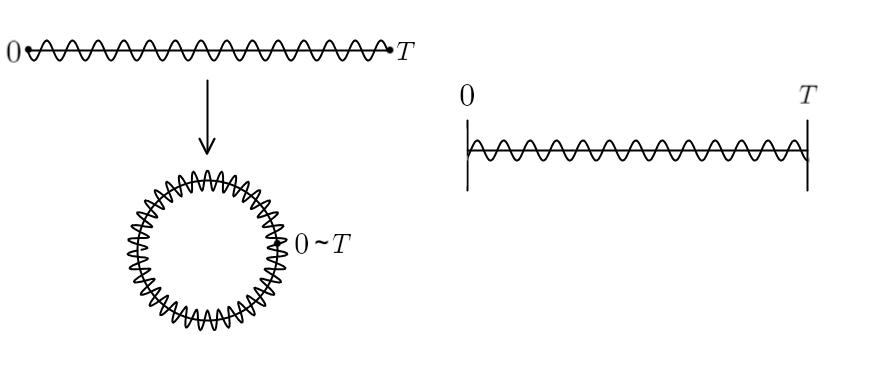
\includegraphics[width=0.7\textwidth]{imgs-MSc-thesis/torus-obc.png}
    \caption{Sketchy representation of the Periodic Boundary Conditions vs \obc\space in time direction}
    \label{fig:torus}
\end{figure}
\newline
The innovative work of Luscher and Schaefer addressed this topological issue.
Until this point, the boundary conditions imposed on Gauge and fermionic fields were Periodic Boundary Conditions (PBC) in both the temporal and spatial directions.
This choice was made in order to achieve temporal and spatial translation invariance.
The modification introduced by Luscher involved \obc\space in time direction with the natural consequence of the breaking of time translation symmetry.
A sketchy representation of the topological differences is shown in Figure \ref{fig:torus}.
The conditions to impose on fields are \cite{OBC_top}:
\begin{equation*}
    \begin{gathered}
        F_{0i}(\vec x, x_4=0) = F_{0i}(\vec x, x_4=T) = 0 \qquad \forall i = 1,2,3 \\
        \begin{aligned}
            & P_+ \psi (\vec x, 0) = P_- \psi (\vec x, T) = 0 \\
            & \bar\psi (\vec x, 0) P_- = \bar\psi (\vec x, T) P_+ = 0 
        \end{aligned}
        \quad\quad P_{\pm} = \frac{1}{2}\left(\mathbb{I} \pm \gamma_5 \right)
    \end{gathered}
\end{equation*}
The peculiar conditions on fermion fields are chosen in order to achieve parity and time reflection.
In Appendix \ref{app:connection} I report a proof of the connection of the space of Gauge fields defined with the new boundary conditions.
This connection of the space solves - not at all - the problem of large scaling of autocorrelation times.
With this choice, the scaling behaviour of some observables comes out to scale $\propto a^{-2}$, instead of $\propto a^{-5}$.
There is a variety of papers confirming that \obc\space decrease autocorrelation times.
For example, look at the following table from \cite{Topology-WilsonFlow-HMC}:
\begin{figure}[h!]
    \centering
    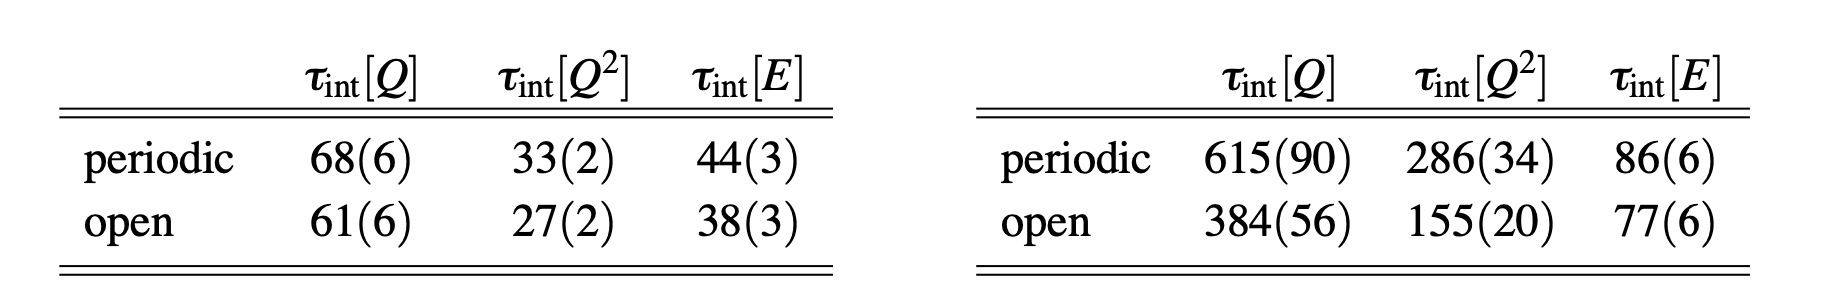
\includegraphics[width=0.9\textwidth]{imgs-MSc-thesis/autocorrelation.png}
    \caption{Comparison of autocorrelation times measured on lattices with periodic and open boundary conditions in time direction.
    The table on the left refers to a latiice with $a=0.1$ fm. The one on the right to a lattice with $a=0.07$ fm. The difference between OBC and PBC increases as the lattice spacing tends to zero. \cite{Topology-WilsonFlow-HMC}}
    \label{tab:autocorrelation-times}
\end{figure}
\newline
Another aspect to keep in mind follows.
The formulation of lattice quantum physics with OBC in this case remains the same in the bulk\footnote{``bluk'': the sub-lattice from which the boundaries with $x_4 = 0, x_4 = T$ are removed}.
However, the vacuum state $|\Omega\ra$ at the time boundaries differs from the vacuum state $|0\ra$ in the bulk, which represents the physical vacuum.
It is proven \cite{OBC_top} that both vacuum states possess the physical vacuum quantum numbers.
Thus a formulation of Lattice QFT similar to the case of periodic boundary conditions is allowed.
Given a local operator of the fields $\mathcal{X}(x_1,\dots,x_n)$, its vacuum expectation value is defined in the following way:
\begin{equation*}
    \la \mathcal{X}(x_1,\dots,x_n) \ra = \la \Omega | T \left\{ \mathcal{X}(x_1,\dots,x_n) \right\} | \Omega \ra
\end{equation*}
The formalism of transfer matrix $\mathbb{T} = e^{-a\hat H}$ is still valid.
A good reference that explains how to treat vacuum expectation values of observables is \cite{ExtractionSpectralQuantities}.
The same topic - along with some generalizations to three point correlators - is presented at the end of the Chapter \ref{ch:operators}.

\subsection{Linking OBC with absence of Wilson-Dirac zero modes}
\noindent
In this subsection I want to justify the use of \obc\space to simulate sea configurations and explain how they protect the sea fields against Wilson-Dirac zero modes.
In fact, from this perspective, OBC could represent a smart alternative to tmQCD.
\newline 
One of the primary purposes of lattice QFT simulations is the evaluation of low-energy QCD quantities.
To accurately describe the sea sector in low-energy QCD, the minimal quark content required is the doublet $(u, d)$.
In this case tmQCD represents a very good regularization choice for the sea sector for the reasons described in \ref{subsec:zero-modes}, in particular because it provides a non null fermion determinant.
\newline
A further step could be the introduction of the {\it strange} quark in sea sector.
However, its description through tmQCD regularization is only feasible when coupled to the {\it charm} quark.
From an ideal perspective, it can be a good solution, but the insertion of a fourth quark flavour represents a computational challenge.
Moreover, the mass $m_c$ is sufficiently large to make the $c$ quark uneffective at energies below $\Lambda_{\text{QCD}}$.
In theoretical particle physics it is said ti be ``integrated out''.
The best compromise between computational advantage and physical content seems to be the set of $(u,d,s)$ quarks in the sea.
\newline
Therefore, the key question arises: \textit{How can we simulate $N_f = 2+1$ sea flavours while avoiding the Dirac-Wilson zero modes?}
It is precisely at this point that \obc\space emerge as a powerful alternative to twisted mass QCD. 
In fact the use of OBC in the quark fields
\begin{equation}\label{eq:obc-on-fermions}
    \begin{aligned}
        & P_+ \psi (\vec x, 0) = P_- \psi (\vec x, T) = 0 \\
        & \bar\psi (\vec x, 0) P_- = \bar\psi (\vec x, T) P_+ = 0 
    \end{aligned}
    \quad\quad P_{\pm} = \frac{1}{2}\left(\mathbb{I} \pm \gamma_5 \right)
\end{equation}
protects the theory from zero modes of th Wislon-Dirac operator.
The proof is reported in a paper by S. Luscher \cite{SF-luscher}, one of the creators of the \obc.
\newline
At this stage, it should be clear why sea quark action (\ref{eq:sea-action}) does not make use of twisted mass terms:
\begin{itemize}
    \item [(i)] The \oait\space is guaranteed by the SW term.
    \item [(ii)] The \obc\space provide a protection against zero modes.
\end{itemize}
Hence the same attributes of tmQCD are achieved, albeit through different ways.

%%%%%%%%%%%%%%%%%%%%%%%%%%%%%%%%%%%%%%%%%%%%%%%%%%%%%%%%%%%%%%%%%%%%%%%%%%%%%%%%%%%%%%%%%
%%%%%%%%%%%%%%%%%%%%%%%%%%%%%%%%%%%%% THIRD CHAPTER %%%%%%%%%%%%%%%%%%%%%%%%%%%%%%%%%%%%%
%%%%%%%%%%%%%%%%%%%%%%%%%%%%%%%%%%%%%%%%%%%%%%%%%%%%%%%%%%%%%%%%%%%%%%%%%%%%%%%%%%%%%%%%%
\chapter{Operators $\Theta_i^{[+]}$s on the lattice and $B_i$ extraction}\label{ch:operators}
\lettrine[lines=2, findent=3pt, nindent=0pt]{T}{}he previous chapter outlined the general framework of lattice QCD, paying particular attention to the regularization employed in the present work.
In this chapter such peculiar regularization is used to build the mixing operators $\{\Theta_i\}$ on the lattice.
Some properties of the discretized lattice operators are described.
Such properties consist in:
\begin{enumerate}
    \item An automatic \oait\space of two and three points meson correlators with no need of multiple simulations (Wilson average) or other specific strategies.
        Such correlators are required to extract matrix elements $\la \bar K^0 | \Theta_i^{[+]} | K^0 \ra$ or bag parameters.
    \item The absence of wrong chirality mixing of operators $\{ \Theta_i^{[\pm]} \}$ in renormalization procedure.
        In principle they should mix because Wilson term in action (\ref{eq:valence-action}) explicitly breaks chiral symmetry.
        Despite the symmetry breaking, this mixing comes out to be absent for symmetry reasons.
    \item A specific basis choice for the operators that gives a blocks-like renormalization matrix $Z_{ij}$, which simplify the renormalization procedure.
\end{enumerate}

\noindent
In order to achieve these properties, some reformulations of the operators and strategies are required.
The initial and majority of the chapter is dedicated to describing the four-fermion, dimension-six, mixing operators on the lattice. 
The second part of the chapter is reserved to a detailed description of the strategy to extract bag parameters and matrix elements $\la \bar K^0 | \Theta_i^{[+]} | K^0 \ra$ from two and three points correlators.


\section{Continuum $\Theta_i^{[\pm]}$s and the new operators $Q_i^{[\pm]}$s}
\noindent
The SUSY operator basis for \kkb oscillations was introduced in (\ref{eq:Thetai-operators}).
Despite its historical significance, the basis $\{\Theta_i\}$ will be replaced by another basis $\{Q_i\}$ because of its particular renormalization properties.
However, before introducing this new basis, I need to present some modifications to the ``old'' SUSY basis.
\newline
I aim to reformulate operators $\Theta_3$ and $\Theta_5$ by rearranging the spin and colour indices contractions within the same couple of quarks. 
This can be done by applying the Fierz relations \cite{Itzykson-Zuber} along with calculation of $\Theta_{3,5}$, as outlined in Appendix \ref{app:fierz}.
The new set of operators comes out to be:
\begin{equation*}
    \begin{aligned}
        & \Theta_1 = \Big[\bar s^a \gamma_\mu (1+\gamma_5) d^a \Big]\Big[ \bar s^b \gamma_\mu (1+\gamma_5) d^b \Big] \\
        & \Theta_2 = \Big[\bar s^a  (1+\gamma_5) d^a \Big]\Big[ \bar s^b (1+\gamma_5) d^b \Big] \\
        & \Theta_3 = -\Big[\bar s^a  P_R d^a \Big]\Big[ \bar s^b d^b \Big] - \Big[\bar s^a P_R d^a \Big]\Big[ \bar s^b \gamma_5 d^b \Big] + \Big[\bar s^a P_R \sigma_{\mu\nu} d^a \Big]\Big[ \bar s^b \sigma_{\mu\nu} d^b \Big] \\ 
        & \Theta_4 = \Big[\bar s^a  (1+\gamma_5) d^a \Big]\Big[ \bar s^b (1-\gamma_5) d^b \Big] \\
        & \Theta_5 = -\Big[\bar s^a  P_R\gamma_\mu d^a \Big]\Big[ \bar s^b \gamma_\mu d^b \Big] - \Big[\bar s^a P_R \gamma_\mu \gamma_5 d^a \Big]\Big[ \bar s^b \gamma_\mu\gamma_5 d^b \Big] \\
     \end{aligned}
\end{equation*}
where $\{\tilde\Theta_i\}$ are omitted.
From this point on the notation described in Appendix \ref{app:notations} is used.
The shortway to write the above operators is:
\begin{equation*}
    \begin{aligned}
        & \Theta_1 = VV + AA +VA +AV \\
        & \Theta_2 = SS + PP + SP + PS \\
        & \Theta_3 = \frac{1}{2}\left( -SS-PS-SP-PP+TT+\tilde{T}T \right) \\
        & \Theta_4 = SS + PS - SP - PP \\
        & \Theta_5 = \frac{1}{2}\left(-VV+AV-VA+AA\right) \\
     \end{aligned}
\end{equation*}
Then the parity even parts $\{\Theta_i^{[+]}\}$ and parity odd parts $\{\Theta_i^{[-]}\}$ are:
\begin{equation}\label{eq:Theta_i-final}
    \begin{split}
        & \Theta_1^{[+]} = VV + AA \\
        & \Theta_2^{[+]} = SS + PP \\
        & \Theta_3^{[+]} = \frac{1}{2}\left(-SS-PP +TT\right) \\
        & \Theta_4^{[+]} = SS - PP \\
        & \Theta_5^{[+]} = \frac{1}{2}\left(AA-VV\right) \\
    \end{split}
  \qquad\qquad
    \begin{split}
        & \Theta_1^{[-]} = VA + AV \\
        & \Theta_2^{[-]} = SP + PS \\
        & \Theta_3^{[-]} = \frac{1}{2}\left(-SP-PS +\tilde{T}T\right) \\
        & \Theta_4^{[-]} = PS - SP \\
        & \Theta_5^{[-]} = \frac{1}{2}\left(AV-VA\right) \\
    \end{split}
\end{equation}
For reasons that will be clear later in this chapter, I introduce a new basis $\{Q_i^{[\pm]}\}$ of parity even and parity odd operators \cite{DoniniMartinelliOperators}:
\begin{equation}\label{eq:Q_i-continuum}
    \begin{split}
        & Q_1^{[+]} = VV + AA \\
        & Q_2^{[+]} = VV - AA \\
        & Q_3^{[+]} = SS - PP \\
        & Q_4^{[+]} = SS + PP \\
        & Q_5^{[+]} = TT \\
    \end{split}
  \qquad\qquad\qquad
    \begin{split}
        & Q_1^{[-]} = VA + AV \\
        & Q_2^{[-]} = VA - AV \\
        & Q_3^{[-]} = PS - SP \\
        & Q_4^{[-]} = PS + SP \\
        & Q_5^{[-]} = \tilde{T}T \\
    \end{split}
\end{equation}
Once evaluated the matrix elements $\la \bar K^0 | Q_i^{[\pm]} | K^0 \ra$, the elements $\la \bar K^0 | \Theta_i^{[\pm]} | K^0 \ra$ can be recovered by applying:
\begin{equation*}
    \begin{split}
        & \Theta_i^{[\pm]} = \Lambda_{ij} Q_j^{[\pm]}  \text{ and}\\
        & \la \bar K^0 | \Theta_i^{[\pm]} | K^0 \ra =\Lambda_{ij} \la \bar K^0 | Q_j^{[\pm]} | K^0 \ra
    \end{split}
    \qquad\qquad
    \Lambda_{ij} = 
    \begin{pmatrix}
        1 & 0 & 0 & 0 & 0 \\
        0 & 0 & 0 & 1 & 0 \\
        0 & 0 & 0 & -\frac{1}{2} & +\frac{1}{2} \\
        0 & 0 & 1 & 0 & 0 \\
        0 & -\frac{1}{2} & 0 & 0 & 0 \\
    \end{pmatrix}
\end{equation*}
The $\{Q_i^{[\pm]}\}$ operators possess a relevant advantage with respect to the $\{\Theta_i^{[\pm]}\}$:
once regularized as outlined in this chapter, they have renormalization mixing properties that simplify the evaluation of renormalized operators and renormalization constants.
This will be better explained in \ref{sec:renormalization-properties}.
\newline
I will show in section \ref{sec:asympt-behav} how the bag parameters can be extracted from two and three points correlators.
Firstly, I introduce such correlators\footnote{To be precise, these are not the usual $n-$points correlators but their projections over null momenta.} in continuum QFT:
\begin{equation}\label{eq:3pts-correlators}
    C_i^\text{QCD}(x_4,y_4,z_4) = \int d^3y \hspace*{.3mm} d^3z \left\la \bar K^0(x) Q_i(y) \bar K^0(z) \right\ra
\end{equation}
\begin{equation*}
    G_{K^0 \bar K^0}^\text{QCD}(x_4,y_4) = \int d^3y \left\la \bar K^0(x) K^0(y) \right\ra
\end{equation*}
\begin{equation*}
    X_{\bar K^0}^\text{QCD}(x_4,y_4) = \int d^3y \left\la A_0^{(\bar d s)}(x) \bar K^0(y) \right\ra
\end{equation*}
The source operators $\bar K^0$ and $K^0$ are defined in Chapter \ref{chap:kaons} as the pseudoscalar densities of $d$ and $s$ doublet of quarks, while the superscript QCD stresses that these are the correlation functions in continuum quantum chromodynamics.
The current $A_\mu^{(\bar d s)} = \bar d \gamma_\mu \gamma_5 s $ is the axial current associated to Kaons. 
The amplitudes $$\mathcal{A}_i^\text{QCD} = \la \bar K^0 | Q_i^{[+]} | K^0 \ra$$ needed for the bag parameters are isolated from higher mass states contributions by considering asymptotic behaviour of correlators for $0 \ll z_4 \ll y_4 \ll x_4 \ll T$.
So the condition $x_4 > y_4 > z_4$ is supposed to be always satisfied.
The full discussion about the extraction is left to section \ref{sec:asympt-behav}.

\section{Flavour replicas on the lattice}
\noindent
The regularized action (\ref{eq:valence-action}) contains replicas of the $d$ and $s$ flavours, then the entire set of valence quarks is $u,d,d',s,s'$.
The choice of multiple quarks of the same flavour comes from \cite{FR2}  and is formulated to achieve specific properties of the three-point correlators;
such properties are outlined in section \ref{sec:operators-properties}.
I refer to the model with flavour replicas as the FR model (::Flavour Replicas).
\newline
I focus on \textit{how} the FR model must be built in order to simulate the same flavour content of the standard QCD (simply named QCD).
Specifically, I aim to construct three points correlators in the FR model such that they yield the same Wick contractions of functions (\ref{eq:3pts-correlators}).
The proof is given below.

\subsection{Proof of equivalence of Wick contractions}
\noindent
Let's consider a general three points correlator in standard QCD:
\begin{equation*}
    G^\text{QCD}(x,y,z) = \left\la \bigg(\bar d(x) \Gamma_\xi s(x)\bigg) \bigg(\bar s(y) \Gamma_\rho d(y) \bar s(y) \Gamma_\sigma d(y)\bigg) \bigg(\bar d(z) \Gamma_\omega s(z)\bigg) \right\ra
\end{equation*}
with $\Gamma_{\xi,\rho,\sigma,\omega}$ some matrices in spin space.
The correlation functions (\ref{eq:3pts-correlators}) are nothing but the sum over spatial components of the above quantity.
The Wick contractions of such correlator follow:\footnote{I use the pedsubscripts $c,d$ to refer to connected or disconnected diagrams}:
\begin{equation*}
    \begin{split}
        & G_{d1}^\text{QCD}(x,y,z): \wick{\c1{\bar d (x)} \Gamma_\xi \c2{s(x)} \cdot \c2{\bar s (y)} \Gamma_\rho \c1{d (y)} \cdot \c1{\bar s (y)} \Gamma_\sigma \c2{d(y)} \cdot \c2{\bar d (z)} \Gamma_\omega \c1{s (z)} } \\
        & G_{d2}^\text{QCD}(x,y,z): \wick{\c1{\bar d (x)} \Gamma_\xi \c2{s(x)} \cdot \c3{\bar s (y)} \Gamma_\rho \c4{d (y)} \cdot \c2{\bar s (y)} \Gamma_\sigma \c1{d(y)} \cdot \c4{\bar d (z)} \Gamma_\omega \c3{s (z)} } \\
        & G_{c1}^\text{QCD}(x,y,z): \wick{\c1{\bar d (x)} \Gamma_\xi \c2{s(x)} \cdot \c2{\bar s (y)} \Gamma_\rho \c3{d (y)} \cdot \c4{\bar s (y)} \Gamma_\sigma \c1{d(y)} \cdot \c3{\bar d (z)} \Gamma_\omega \c4{s (z)} } \\
        & G_{c2}^\text{QCD}(x,y,z): \wick{\c1{\bar d (x)} \Gamma_\xi \c2{s(x)} \cdot \c4{\bar s (y)} \Gamma_\rho \c1{d (y)} \cdot \c2{\bar s (y)} \Gamma_\sigma \c3{d(y)} \cdot \c3{\bar d (z)} \Gamma_\omega \c4{s (z)} } \\
    \end{split}
\end{equation*}
They generates single or double traces functions:
\begin{equation}\label{eq:wick-contractions-general}
    \begin{split}
        & G_{d1}^\text{QCD}(x,y,z) = \left\la \tr \Big[ \Gamma_\xi S_{s} (x,y) \Gamma_\rho S_{d} (y,x) \Big] \hspace*{.5mm} \tr \Big[ \Gamma_\omega S_{s} (z,y) \Gamma_\sigma S_{d} (y,z) \Big] \right\ra \\
        & G_{d2}^\text{QCD}(x,y,z) = \left\la \tr \Big[ \Gamma_\xi S_{s} (x,y) \Gamma_\sigma S_{d} (y,x) \Big] \hspace*{.5mm} \tr \Big[ \Gamma_\omega S_{s} (z,y) \Gamma_\rho S_{d} (y,z) \Big] \right\ra \\
        & G_{c1}^\text{QCD}(x,y,z) = - \left\la \tr \Big[ \Gamma_\xi S_{s} (x,y) \Gamma_\rho S_{d} (y,z) \Gamma_\omega S_{s} (z,y) \Gamma_\sigma S_{d} (y,x) \Big] \right\ra \\
        & G_{c2}^\text{QCD}(x,y,z) = - \left\la \tr \Big[ \Gamma_\xi S_{s} (x,y) \Gamma_\sigma S_{d} (y,z) \Gamma_\omega S_{s} (z,y) \Gamma_\rho S_{d} (y,x) \Big] \right\ra \\
    \end{split}
\end{equation}
then the total contribution to $G^\text{QCD}(x,y,z)$ is given by:
\begin{equation*}
    G^\text{QCD}(x,y,z) = G_{d1}^\text{QCD}(x,y,z) + G_{d2}^\text{QCD}(x,y,z) + G_{c1}^\text{QCD}(x,y,z) + G_{c2}^\text{QCD}(x,y,z)
\end{equation*}
I want to replicate this contributions using the new flavours $d,d',s,s'$ built on the lattice.
The strength of this method lies in the fact that primed and unprimed flavours cannot contract with each other.
Therefore I can build an appropriate operator for each contraction.
I define an antikaon source in $x$ with primed flavours $\bar d' (x) \Gamma_\xi s'(x)$ and another in $z$ with unprimed flavours $\bar d (z) \Gamma_\omega s(z)$.
The intermediate operator is replaced by: 
\begin{equation*}
    \begin{aligned}
        \Phi_{\rho,\sigma}(y) = 
        & \bar s(y) \Gamma_\rho d(y) \bar s'(y) \Gamma_\sigma d'(y) + \bar s(y) \Gamma_\sigma d(y) \bar s'(y) \Gamma_\rho d'(y) + \\
        & + \bar s(y) \Gamma_\rho d'(y) \bar s'(y) \Gamma_\sigma d(y) + \bar s(y) \Gamma_\sigma d'(y) \bar s'(y) \Gamma_\rho d(y)
    \end{aligned}
\end{equation*}
In this case the correlator:
\begin{equation*}
    G^\text{FR}(x,y,z) = \left\la \bar d' (x) \Gamma_\xi s'(x) \Phi_{\rho,\sigma}(y) \bar d (z) \Gamma_\omega s(z) \right\ra
\end{equation*}
gives only one contraction for each term of $\Phi_{\rho,\sigma}(y)$, thus four contractions identical to equations (\ref{eq:wick-contractions-general}) up to primed flavours.
Such contractions are labeled by $G_{d1}^\text{FR}, G_{d2}^\text{FR}, G_{c1}^\text{FR}, G_{c2}^\text{FR}$ and are shown in Figure \ref{fig:contractions-general}.
\begin{figure}[h!]
    \centering
    \begin{subfigure}[b]{0.49\textwidth}
        \centering
        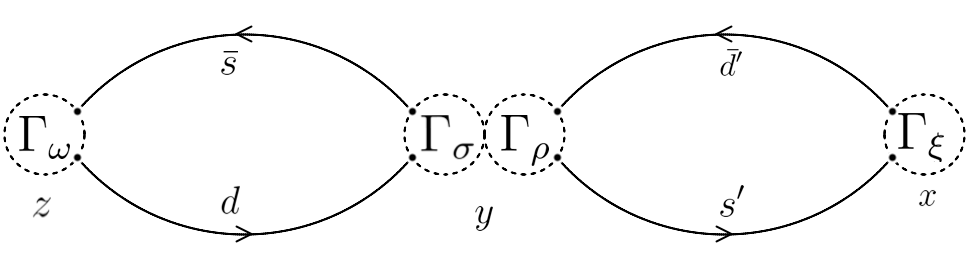
\includegraphics[width=\textwidth]{imgs-MSc-thesis/Wick_D1.png}
        \caption{$G_{d1}^\text{FR}(x,y,z)$}
    \end{subfigure}
    \begin{subfigure}[b]{0.49\textwidth}
        \centering
        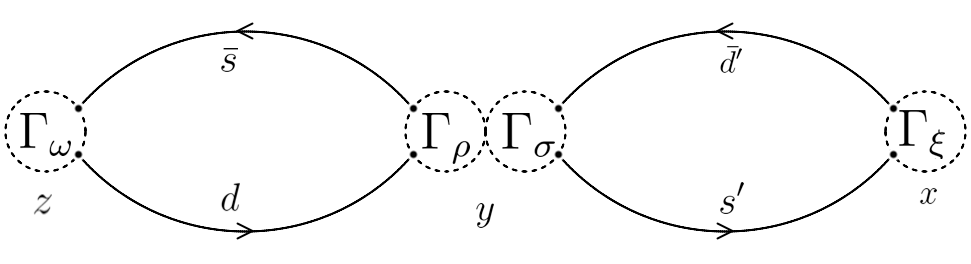
\includegraphics[width=\textwidth]{imgs-MSc-thesis/Wick_D2.png}
        \caption{$G_{d2}^\text{FR}(x,y,z)$}
    \end{subfigure}
    \begin{subfigure}[b]{0.49\textwidth}
        \centering
        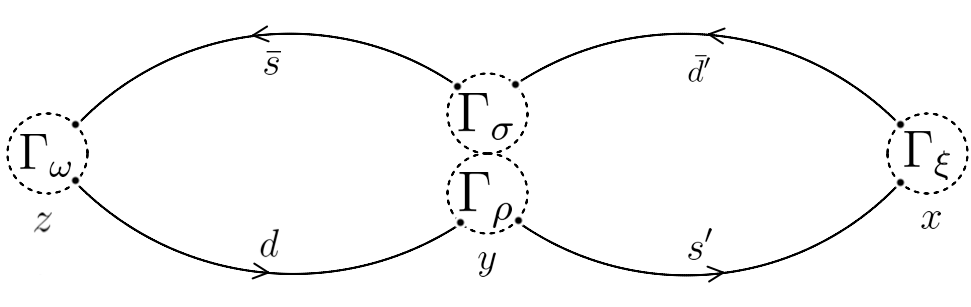
\includegraphics[width=0.95\textwidth]{imgs-MSc-thesis/Wick_C1.png}
        \caption{$G_{c1}^\text{FR}(x,y,z)$}
    \end{subfigure}
    \begin{subfigure}[b]{0.49\textwidth}
        \centering
        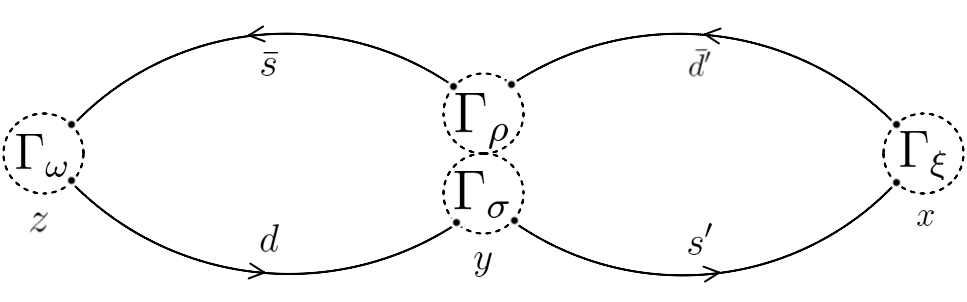
\includegraphics[width=0.95\textwidth]{imgs-MSc-thesis/Wick_C2.png}
        \caption{$G_{c2}^\text{FR}(x,y,z)$}
    \end{subfigure}
    \caption{Wick contractions that contribute to the correlator $G^\text{FR}(x,y,z)$ in the framework of QCD with flavours replicas.}
    \label{fig:contractions-general}
\end{figure}

\section{From physical basis to twisted basis}
\noindent
Thanks to the previous proof, the parity even operators $Q_{i}^{[+]}$ (equation (\ref{eq:Q_i-continuum})) can be built on the lattice in the FR framework by introducing four different flavours.
The flavours used are the lattice regularized Osterwalder-Seiler quarks, as described in previous Chapter.
The following notation for valence flavours is adopted:
\begin{equation*}
    \begin{aligned}
        \text{physical OS basis:}
        & \quad \chi^1 = s_\text{ph} \qquad \chi^3 = s'_\text{ph} \\
        & \quad \chi^2 = d_\text{ph} \qquad \chi^4 = d'_\text{ph} \\
        \text{twisted OS basis: }
        & \quad \psi^1 = s_\text{tw} \qquad \psi^3 = s'_\text{tw} \\
        & \quad \psi^2 = d_\text{tw} \qquad \psi^4 = d'_\text{tw} \\
    \end{aligned}
    \qquad
    \text{with } \chi^i = \mathbf{J}(\pi/2,r_i)\psi^i
\end{equation*}
The operators $Q_{i}^{[+]}$ in continuum QCD are replaced by the new operators $O_{i,[+]}^\text{phys}$ in the lattice QCD fermion physical basis:
\begin{equation*}
    \begin{split}
        & O_{1[+]}^\text{phys} = 2 \left\{\big[\bar\chi^1 \gamma_\mu \chi^2 \big] \big[\bar\chi^3 \gamma_\mu \chi^4 \big] + \big[ \bar\chi^1 \gamma_\mu \gamma_5 \chi^2 \big] \big[ \bar\chi^3 \gamma_\mu \gamma_5 \chi^4 \big] + \left(2\leftrightarrow 4\right)\right\} \\
        & O_{2[+]}^\text{phys} = 2 \left\{\big[\bar\chi^1 \gamma_\mu \chi^2 \big] \big[\bar\chi^3 \gamma_\mu \chi^4 \big] - \big[ \bar\chi^1 \gamma_\mu \gamma_5 \chi^2 \big] \big[ \bar\chi^3 \gamma_\mu \gamma_5 \chi^4 \big] + \left(2\leftrightarrow 4\right)\right\} \\
        & O_{3[+]}^\text{phys} = 2 \left\{\big[\bar\chi^1 \chi^2 \big] \big[ \bar\chi^3 \chi^4 \big] - \big[ \bar\chi^1 \gamma_5 \chi^2 \big] \big[ \bar\chi^3 \gamma_5 \chi^4\big] + \left(2\leftrightarrow 4\right)\right\} \\
        & O_{4[+]}^\text{phys} = 2 \left\{\big[\bar\chi^1 \chi^2 \big] \big[ \bar\chi^3 \chi^4 \big] + \big[ \bar\chi^1 \gamma_5 \chi^2 \big] \big[ \bar\chi^3 \gamma_5 \chi^4\big] + \left(2\leftrightarrow 4\right)\right\} \\
        & O_{5[+]}^\text{phys} = 2 \left\{\big[\bar\chi^1 \sigma_{\mu\nu} \chi^2 \big] \big[ \bar\chi^3 \sigma_{\mu\nu} \chi^4 \big] + \left(2\leftrightarrow 4\right)\right\} \\
    \end{split}
\end{equation*}
According to what is explained in section \ref{sec:OS-regularization}, I need to transform the operators from the physical to twisted basis.
To do that I apply the OS rotations $\mathbf{J}(\pi/2,r_i)$ and I remember that:
\begin{equation*}
    r_1 = r_2 = r_3 = - r_4 = \pm 1
\end{equation*}
It could be useful to use cases {\bf \# 1} (formula (\ref{eq:OS-twisted-currents-equal-r})) and {\bf \# 2} (formula (\ref{eq:OS-twisted-currents-defferent-r})) derived in Appendix \ref{app:physical-basis}.
The resulting operators are the following:
\begin{equation}\label{eq:O_i-operators-twisted-final}
    \begin{split}
        & O_{1[+]}^\text{tw} = \mp 2i \left\{\big[\bar\psi^1 \gamma_\mu \psi^2 \big] \big[\bar\psi^3 \gamma_\mu \gamma_5 \psi^4 \big] + \big[ \bar\psi^1 \gamma_\mu \gamma_5 \psi^2 \big] \big[ \bar\psi^3 \gamma_\mu \psi^4 \big] + \left(2\leftrightarrow 4\right)\right\} \\
        & O_{2[+]}^\text{tw} = \mp 2i \left\{\big[\bar\psi^1 \gamma_\mu \psi^2 \big] \big[\bar\psi^3 \gamma_\mu \gamma_5 \psi^4 \big] - \big[ \bar\psi^1 \gamma_\mu \gamma_5 \psi^2 \big] \big[ \bar\psi^3 \gamma_\mu \psi^4 \big] - \left(2\leftrightarrow 4\right)\right\} \\
        & O_{3[+]}^\text{tw} = \pm 2i \left\{\big[\bar\psi^1 \gamma_5 \psi^2 \big] \big[ \bar\psi^3 \psi^4 \big] - \big[ \bar\psi^1 \psi^2 \big] \big[ \bar\psi^3 \gamma_5 \psi^4\big] - \left(2\leftrightarrow 4\right)\right\} \\
        & O_{4[+]}^\text{tw} = \pm 2i \left\{\big[\bar\psi^1 \gamma_5 \psi^2 \big] \big[ \bar\psi^3 \psi^4 \big] + \big[ \bar\psi^1 \psi^2 \big] \big[ \bar\psi^3 \gamma_5 \psi^4\big] + \left(2\leftrightarrow 4\right)\right\} \\
        & O_{5[+]}^\text{tw} = \pm 2i \left\{\big[\bar\psi^1 \tilde\sigma_{\mu\nu} \psi^2 \big] \big[ \bar\psi^3 \sigma_{\mu\nu} \psi^4 \big] + \big[\bar\psi^1 \sigma_{\mu\nu} \psi^4 \big] \big[ \bar\psi^3 \tilde\sigma_{\mu\nu} \psi^2 \big] \right\} \\
    \end{split}
\end{equation}
where the signs $\pm,\mp$ depend on the choice of $r_1=\pm1$.
The other quantities that need to be twisted are the Kaon sources:
\begin{equation}\label{eq:kaon-sources}
    \begin{gathered}
        \bar K^{0} = P^\text{phys}_{21} = \bar\chi^2 \gamma_5 \chi^1 = \pm i \bar\psi^2 \psi^1 = \pm i S^\text{tw}_{21} \\
        \bar K^{'0} = P^\text{phys}_{43} = \bar\chi^4 \gamma_5 \chi^3 = \bar\psi^4 \gamma_5 \psi^3 = P^\text{tw}_{43} \\
    \end{gathered}
\end{equation}
It is notable that the OS twist maps the parity even operators into parity odd ones.
However also the source $K^{0}$ changes parity, then the overall sign of the correlator under $\mathbb{P}$ is preserved and equal to $+1$, as strong interactions should do.
Now the work in Maximally twisted OS valence QCD is well defined and, by construction, the correlation functions:
\begin{equation}\label{eq:lattice-correlators}
    C_i^\text{FR}(x_4,y_4,z_4) = \pm i a^6 \sum_{\vec x, \vec y, \vec z}\left\la \left(\bar\psi^4 \gamma_5 \psi^3 \right) (x) O_{i[+]}^\text{tw} (y) \left(\bar\psi^2 \psi^1 \right) (z)\right\ra
\end{equation}
give the same Wick contractions of the correlators in equation (\ref{eq:3pts-correlators}), showed in Figure \ref{fig:contractions-general}.
To be rigorous, in this definition there is one more sum with respect to equation (\ref{eq:3pts-correlators}).
This additive sum over $\vec x$ is a (sort of) statistical average and it is used to give more precise results in the simulation.
Similarly, the integrated two points correlation functions are:
\begin{equation}\label{eq:lattice-propagators}
    \begin{split}
        & G_{34}^\text{FR}(x_4,y_4) = a^3 \sum_{\vec x, \vec y} \left\la \left(\bar\psi^4 \gamma_5 \psi^3 \right) (x) \left(\bar\psi^3 \gamma_5 \psi^4 \right) (y) \right\ra \\
        & G_{12}^\text{FR}(x_4,y_4) = - a^3 \sum_{\vec x, \vec y} \left\la \left(\bar\psi^2 \psi^1 \right) (x) \left(\bar\psi^1 \psi^2 \right) (y) \right\ra \\
    \end{split}
\end{equation}
the use of the first or the second correlator is - in principle - equivalent, since one consists in the ``flavour replica'' of the other and vice versa.
Both describe a neutral anti-Kaon $\bar K^0$ propagator.
Nevertheless there are lattice artefacts due to the different regularizations of $d,d'$ that make the pseudoscalar densities $\bar K^0$ and $\bar K^{'0}$ generate slightly different Kaons.
\newline 
Similar definitions hold for $G_{21}^\text{FR}$ and $G_{43}^\text{FR}$.
They differ from (\ref{eq:lattice-propagators}) by an exchange of flavours $(1\leftrightarrow 2)$ or $(3\leftrightarrow 4)$ and correspond to the propagator of the kaon $K^0$ instead of an antikaon $\bar K^0$.
\newline
At the end of the chapter I will use two other correlators to extract the parameter $B_K$, following the method explained in \cite{B_k-extrapolation}:
\begin{equation}\label{eq:axial-correlators}
    \begin{split}
        X_{34}^\text{FR}(x_4,y_4) & = a^3 \sum_{\vec x, \vec y} \left\la A_{0,43}^\text{phys} (x) P_{34}^\text{phys} (y) \right\ra = \pm i a^3 \sum_{\vec x, \vec y} \left\la V_{0,43}^\text{tw} (x) P_{34}^\text{tw} (y) \right\ra \\
                                  & = \pm i a^3 \sum_{\vec x, \vec y} \left\la \left( \bar \psi^4 \gamma_0 \psi^3 \right) (x) \left( \bar \psi^3 \gamma_5 \psi^4 \right) (y) \right\ra \\
        X_{12}^\text{FR}(x_4,y_4) & = a^3 \sum_{\vec x, \vec y} \left\la A_{0,21}^\text{phys} (x) P_{12}^\text{phys} (y) \right\ra = \pm i a^3 \sum_{\vec x, \vec y} \left\la A_{0,21}^\text{tw} (x) S_{12}^\text{phys} (y) \right\ra \\
                                  & = \pm i a^3 \sum_{\vec x, \vec y} \left\la \left( \bar \psi^2 \gamma_0 \gamma_5 \psi^1 \right) (x) \left( \bar \psi^1 \psi^2 \right) (y) \right\ra \\
    \end{split}
\end{equation}
where I have used agiain the results in Appendix \ref{app:OSreg}.
These two correlators give, in the continuum limit and in regime of asymptotic behaviour (Section \ref{sec:asympt-behav}), the matrix element $\la 0 | A_0^{(\bar d s)} (x) | \bar K^0 (\vec p) \ra$.

\section{Properties of correlators and $O_{i[+]}$ operators}\label{sec:operators-properties}
\subsection{Automatic \oait}
\noindent
In the first paper by Frezzotti and Rossi \cite{FR1} a strategy to $O(a)-$improve observables based on of Wilson Dirac fermions or twisted fermions has been introduced.
The operation needed to improve the observables is called \textit{Wilson Average} (WA) and it consists of averaging observables evaluated with different signs of Wislon parameters $r_i$.
In a shorthand notation I refer to the set of Wilson parameters of the theory with $R = \{r_1,\dots,r_N\}$.
\newline
Given an observable $\mathcal{X}$ functional of the valence fields and Gauge fields, the WA of its vacuum expectation value is:
\begin{equation*}
    \left\la \mathcal{X} \right\ra\Big|_{WA}^a = \frac{1}{2}\left( \left\la \mathcal{X} \right\ra\Big|_{+R}^a + \left\la \mathcal{X} \right\ra\Big|_{-R}^a\right) 
    = \zeta_\mathcal{X}(R)  \left\la \mathcal{X} \right\ra\Big|^\text{continuum} + O(a^2)
\end{equation*}
where $\zeta_\mathcal{X}(R)$ is a constant, dependent on Wilson parameters, needed to match lattice VEV with continuum VEV.
The proof that the Wilson average gives an \oait\space is reported in \cite{FR1}. 
\newline
The WA method implies that multiple simulations must be done.
However there are particular cases in which this is not necessary because each $\left\la \mathcal{X} \right\ra\big|_{\pm R}^a$ is automatically improved and the WA is not necessary.
This is exactly the case of correlators of the type (\ref{eq:lattice-correlators}) and (\ref{eq:lattice-propagators}).
In fact the valence and sea actions (\ref{eq:valence-action}) and (\ref{eq:sea-action}) admit the spurionic symmetry $\mathbb{P}\x (R\mapsto -R)$.
In particular $\mathbb{P}$ is the parity operation ($\mathbb{P}x = x_p$) and $(R\mapsto -R)$ is the change of signs of the Wilson parameters.
Under this discrete symmetry a correlator of the type (\ref{eq:lattice-correlators}) is mapped into itself because of the symmetry property and it is also mapped into the one with $(R\mapsto -R)$ because of the identity:
\begin{equation*}
    \sum_{\vec x, \vec y, \vec z} f(x,y,z) =  \sum_{\vec x_p, \vec y_p, \vec z_p} f(x_p,y_p,z_p)
\end{equation*}
for any function $f$ of the lattice coordinates.
Then, in simple words, the statement asserts that in this case $\left\la \mathcal{X} \right\ra\big|_{+R}^a = \left\la \mathcal{X} \right\ra\big|_{-R}^a$ and then the WA is not necessary for the \oait.
The same proof can be applied to a simple meson propagator of the type\footnote{about the symbol $\bar\Gamma^\alpha$ see Appendix \ref{app:notations}}:
\begin{equation*}
    G(x,y)=a^3\sum_{\vec x, \vec y} \Big\la \bar \psi^1 (x) \Gamma^\alpha \psi^2 (x) \bar\psi^2 (y) \bar\Gamma^\alpha \psi^1 (y) \Big\ra 
\end{equation*}
and then to two points correlators.
It is important to notice that this proof holds not only for $r_1=r_2=r_3=-r_4$ but for all the possible values of each $r_i$ independently chosen.


\subsection{Renormalization and mixing of operators $O_{i[\pm]}$}\label{sec:renormalization-properties}
\noindent
There are two arguments left to be tested, as mentioned at the very beginning of the chapter.
Both points concern the specific renormalization properties owned by the parity even and parity odd operators $O_{i,[\pm]}^\text{phys}$.
The following has been taken from the paper \cite{DoniniMartinelliOperators}.
\newline
First of all I need notations.
In this section, I will denote generic parity even operators (PE) with the index ${E}$, and generic parity odd operators (PO) with ${O}$.
I define the following quantities:
\begin{equation*}
    \begin{split}
        & \Phi_{AB} = \left( \bar \psi^1 \Gamma^A \psi^2 \right) \left( \bar \psi^3 \Gamma^B \psi^4 \right) \\
        & \Phi_{AB}^F = \left( \bar \psi^1 \Gamma^A \psi^4 \right) \left( \bar \psi^3 \Gamma^B \psi^2 \right) \\
        & \Phi_{AB \pm CD} = \Phi_{AB} \pm \Phi_{CD} \\
        & \Phi_{AB}^\pm = \Phi_{AB} \pm \Phi_{AB}^F \\
    \end{split}
\end{equation*}
In the last definition, note that the signs $\pm$ have nothing to do with parity, but indicate the sign of the flavour exchange.
\newline
To address the mixing issue under renormalization, both natural and accidental symmetries of these operators will be used.
Before that, it must be noted that these operators composed of four quarks
$(i)$ do not mix with higher dimensional operators due to a well known renormalization theorem \cite{Collins} and
$(ii)$ do not mix with lower dimensional operators because it is not possible to replicate four fermions flavour content through lower dimensions less than 6.
As a consequence, I can define a {\it set of four-quarks dimension-6 operators, closed under renormalization procedure} (\ref{eq:closed-set-operators}).
At this point, I define the symmetries used:
\begin{itemize}
    \item Parity $\mathbb{P}$: $\psi^i (x) \mapsto \gamma_4 \psi^i (x_p)$
    \item Charge conjugation $\mathbb{C}$: $\psi^i (x) \mapsto C \left(\bar\psi^{i}\right)^T (x)$
    \item First flavour exchange $\mathbb{S}$: $(\psi^2 \leftrightarrow \psi^4)$
    \item Second flavour exchange $\mathbb{S}'$: $(\psi^1 \leftrightarrow \psi^2, \psi^3 \leftrightarrow \psi^4)$
    \item Third flavour exchange $\mathbb{S}''$: $(\psi^1 \leftrightarrow \psi^4, \psi^2 \leftrightarrow \psi^3)$
\end{itemize}
Clearly, the symmetry $\mathbb{S}$ maps $\Phi$ to $\Phi^F$ and vice versa.
Other useful properties are $\mathbb{S}'' = \mathbb{S}\cdot \mathbb{S}'$, $\mathbb{S}' = \mathbb{S}\cdot \mathbb{S}''$, $\mathbb{S}^2 = 1$.
Next, the following parity even (left column) and parity odd (right column) operators are defined:
\begin{equation}\label{eq:closed-set-operators}
    \begin{split}
        & O_{1,E}^\pm = \Phi^\pm_{VV+AA} \qquad O_{1,O}^\pm = \Phi^\pm_{VA+AV} \\
        & O_{2,E}^\pm = \Phi^\pm_{VV-AA} \qquad O_{2,O}^\pm = \Phi^\pm_{VA-AV} \\
        & O_{3,E}^\pm = \Phi^\pm_{SS-PP} \qquad O_{3,O}^\pm = \Phi^\pm_{PS-SP} \\
        & O_{4,E}^\pm = \Phi^\pm_{SS+PP} \qquad O_{4,O}^\pm = \Phi^\pm_{PS+SP} \\
        & O_{5,E}^\pm = \Phi^\pm_{TT}    \hspace*{40pt} O_{5,O}^\pm = \Phi^\pm_{T\tilde{T}} \\
    \end{split}
\end{equation}
This set consists of 20 operators composed by four fermions and dimensionality 6.
It should be clear that the $O_{i[\pm]}$ used in this work are some operators in the above set.
Below is a table taken from \cite{DoniniMartinelliOperators} that shows how these symmetry transformations act on basis operators.
\begin{table}[ht]
    \centering
    \begin{tabular}{c|ccccc}
        $\Phi_{AB}$ & $\mathbb{P}$ & $\mathbb{CS}'$ & $\mathbb{CS}''$ & $\mathbb{CPS}'$ & $\mathbb{CPS}'' $\\
        \hline
        $\Phi_{VV}$        & $+1$ & $+1$ & $+1$ & $+1$ & $+1$ \\
        $\Phi_{AA}$        & $+1$ & $+1$ & $+1$ & $+1$ & $+1$ \\
        $\Phi_{PP}$        & $+1$ & $+1$ & $+1$ & $+1$ & $+1$ \\
        $\Phi_{SS}$        & $+1$ & $+1$ & $+1$ & $+1$ & $+1$ \\
        $\Phi_{TT}$        & $+1$ & $+1$ & $+1$ & $+1$ & $+1$ \\
        \hline
        $\Phi_{VA}$        & $-1$ & $-1$ & $-\Phi_{AV}$ & $+1$ & $\Phi_{AV}$    \\
        $\Phi_{AV}$        & $-1$ & $-1$ & $-\Phi_{VA}$ & $+1$ & $\Phi_{VA}$    \\
        $\Phi_{SP}$        & $-1$ & $+1$ & $\Phi_{PS}$  & $-1$ & $-\Phi_{PS}$   \\
        $\Phi_{PS}$        & $-1$ & $+1$ & $\Phi_{SP}$  & $-1$ & $-\Phi_{SP}$   \\
        $\Phi_{T\tilde T}$ & $-1$ & $+1$ & $+1$         & $-1$ & $-1$           \\
    \end{tabular}
    \vspace*{.6mm}
    \label{tab:symmetries-of-operators}
    \caption{Transformations acting on operators. The trivial $\mathbb{S}$ transformation and the flavour exchanged operators $\Phi^F$ are not shown.}
\end{table}
\newline
The crux of the proof of the mixing of these operators lies in the fact that the considered transformations are symmetries of the Wilson action and the operators defined above.
Therefore, the quantum numbers - or charges - associated with these symmetries are conserved.
So only operators with the same quantum numbers can mix with each other.
As can be inferred from the table, there is no simplification in the mixing of the PE operators; they all mix with each other.
On the other hand, the situation for the PO operators is different.
The renormalization matrix is a block diagonal matrix:
\begin{equation*}
    \begin{split}
        O_{i,O}^{\pm,\ren} = Z_{ij}^\pm O_{i,O}^{\pm}
    \end{split}
    \qquad\qquad
    Z_{ij} = 
    \begin{pmatrix}
        Z_{11} & 0 & 0 & 0 & 0 \\
        0 & Z_{22} & Z_{23} & 0 & 0 \\
        0 & Z_{32} & Z_{33} & 0 & 0 \\
        0 & 0 & 0 & Z_{44} & Z_{45} \\
        0 & 0 & 0 & Z_{54} & Z_{55} \\
    \end{pmatrix}
\end{equation*}
This greatly simplifies the renormalization process.
About the PE operators, the situation is more complicated, and the reader must refer to the paper \cite{DoniniMartinelliOperators}.
Explicit chiral symmetry breaking introduced by the Wilson term plays a fundamental role and allows the operators to mix their chirality.
However, the matrix elements are \oaid, so even the effects of mixing with wrong chirality have an effect of order $O(a^2)$ or higher.
\newline
To conclude this section, I want to revisit a brilliant reasoning made in \cite{KMBSM}.
For vanishing twisted masses $\mu_i$, the action of Wilson and Osterwalder-Seiler fermions in the twisted basis is indistinguishable.
Therefore, using a massless renormalization scheme, the renormalization properties of the parity odd operators $O_{i[+]}^\text{tw}$ are reflected in those of the parity even operators before the base twist $O_{i[+]}^\text{phys}$.
This result has been formally developed in \cite{FR2}.

\section{Asymptotic behaviours}\label{sec:asympt-behav}
\noindent
The last pending issue of this chapter is the method to isolate the bare amplitudes $\la \bar K^0 | Q_i | K^0 \ra$ in the continuum limit from correlators (\ref{eq:lattice-correlators}) and to extract bag parameters from them.
Such method is based on asymptotic behaviours of correlators at large euclidean times and it is a standard extraction method \cite{montvay-munster}, adapted to the case of \obc\space \cite{ExtractionSpectralQuantities}.
In this section I will consider a generic (integrated) three points correlator of this form:
\begin{equation}\label{eq:correlator-prototype}
    C(x_4,y_4,z_4) = a^6\sum_{\vec x, \vec y, \vec z} \left\la M_A (x) \Xi (y) M_B (z) \right\ra
\end{equation}
where $M_{A}$ and $M_{B}$ are meson sources and $\Xi$ is the intermediate mixing operator.
Againg I suppose $x_4 > y_4 > z_4$.
Notice that the sum over spatial components is a projection over zero momenta of the correlator.
To prove it, let's consider a lattice function $f(\vec x,\vec y,\vec z)$ and its discrete Fourier transform $\tilde{f}(\vec p_x,\vec p_y,\vec p_z)$.
Due to periodic boundary conditions in space directions, the above correlator is space translation invariant.
Thus I suppose $f(\vec x, \vec y, \vec z) = f(0, \vec y - \vec x, \vec z - \vec x)$.
At this point the sum over spatial components is nothing but the discrete Fourier transform calculated in null momenta:
\begin{equation*}
    \begin{gathered}
        \sum_{\vec x, \vec y, \vec z} f(\vec x,\vec y',\vec z') = \mathcal{F}\left[f\right](\vec p_x,\vec p_y,\vec p_z)\bigg|_{\vec p_i = 0} = \sum_{\vec x, \vec y, \vec z} f(0, \vec y - \vec x, \vec z - \vec x) = \\
        = \sum_{\vec x, \vec y', \vec z'} f(\vec 0,\vec y',\vec z') \hspace*{.5mm} \text{exp}\left(i(\vec{p_x}+\vec{p_y}+\vec{p_z})\vec{x}+i\vec{p_y}\cdot\vec{y}'+i\vec{p_z}\cdot\vec{z}' \right)\bigg|_{\vec p_i = 0} = \\
        = \sum_{\vec x} \bar{f}(x'=0, \vec p_y = 0, \vec p_z = 0)
    \end{gathered}
\end{equation*}
where $\bar{f}$ is an intermediate function in which only two of three variables are Fourier transformed.
It is worth noting that a sort of statistical sum over $\vec x$ appears. This will be helpful to reduce noise in data analysis procedure.
The projection over zero momenta is a clever trick because all the involved physical states will have an energy equal to the mass of such state $E=m$ and then a non perturbative extraction of the masses can be done\footnote{In this work there are no mass extractions, but previous papers do it in a very precise way. For example see \cite{LightMesons}\cite{OBC-tm} for $0^{-}$ mesons masses with CLS ensembles.}.
\newline
Now I want to show how the amplitudes can be asymptotically isolated \cite{montvay-munster} from correlator (\ref{eq:correlator-prototype}).
Before of that, a theoretical background in introduced:
\begin{equation*}
    \begin{split}
        & \text{Vacuum state: } \Omega \qquad H|\Omega\ra = 0 \\
        & \text{Other states: } \Psi_{n,p} \qquad H|\Psi_{n,p}\ra = \left(\sum_i E_i(p_i)\right)|\Psi_{n,p}\ra \\
        & \text{Other states projected on zero momenta: } \Psi_{n} \qquad H|\Psi_{n}\ra = \left(\sum_i m_i\right)|\Psi_{n}\ra \\
        & \text{where $i$ runs over the set of particles in the given state.}
    \end{split}
\end{equation*}
I use the transfer matrix formalism to re-express $M_A, M_B$ and $\Xi$:
\begin{equation*}
    \begin{split}
        & \left\la M_A (x)\Xi (y)M_B (z) \right\ra = \left\la \Omega | \mathbb{T}^{T-x_4} M_A (0,\vec x) \mathbb{T}^{x_4-y_4} \Xi (0,\vec y) \mathbb{T}^{y_4-z_4} M_B (0,\vec z) \mathbb{T}^{z_4} | \Omega \right\ra = \\
        & \qquad = \left\la \Omega | e^{-H(T-x_4)} M_A (0,\vec x) e^{-H(x_4-y_4)} \Xi (0,\vec y) e^{-H(y_4-z_4)} M_B (0,\vec z) e^{-Hz_4} | \Omega \right\ra = \\
        & \qquad = \left\la \Omega | M_A (0,\vec x) e^{-H(x_4-y_4)} \Xi (0,\vec y) e^{-H(y_4-z_4)} M_B (0,\vec z) | \Omega \right\ra
    \end{split}
\end{equation*}
I insert a complete set of states between each pair of operators and I use the property of any local operator $\mathcal{O}$:
$$\mathcal{O}(\vec x) = \text{exp}\left(i \vec P \cdot \vec x\right)\mathcal{O}(\vec 0)\text{exp}\left(-i \vec P \cdot \vec x\right)$$
The projection over zero momenta allows to simplify the expression.
The resulting correlator is:
\begin{equation*}
    \begin{split}
        & C(x_4,y_4,z_4) = \\
        & = a^6\sum_{\vec y}\sum_{n,k} \la \Omega | M_A (0) \big[\Psi_n \Psi_n^\dag \big] \Xi (0) \big[\Psi_k \Psi_k^\dag \big] M_B (0) | \Omega \ra \hspace*{0.5mm} e^{-m_n(x_4-y_4)-m_k(y_4-z_4)}
    \end{split}
\end{equation*}
Suppose to consider the case $x_4 \gg y_4 \gg z_4$.
Then, because of the exponentials, only the smallest masses $m_n$ and $m_k$ give a relevant contribution, while all the other states are suppressed.
Supposing that the meson operators $M_A$ and $M_B$ interpolate some single meson states $\Psi_A$ and $\Psi_B$:
\begin{equation}\label{eq:asymptotic-behav-3pts}
    \begin{split}
        & C(x_4,y_4,z_4)\approx \\
        & \qquad \approx  a^6\sum_{\vec y} \la \Omega | M_A(0) | \Psi_A \ra \la \Psi_A | \Xi (0) | \bar\Psi_B \ra \la \bar\Psi_B | M_B (0) | \Omega \ra \hspace*{.5mm} e^{-m_A(x_4-y_4)-m_B(y_4-z_4)}
    \end{split}
\end{equation}
I can follow the same procedure applied to the two points correlation function with meson operators, i.e. the non perturbative meson propagator:
\begin{equation}\label{eq:2pts-correlator-meson}
    G_{C\bar C}(x_4,y_4) = a^3 \sum_{\vec x, \vec y} \la M_C (x) \bar M_C (y) \ra
\end{equation}
For $x_4 \gg y_4$ it can be proved that the asymptotic behaviours of such correlator is:
\begin{equation}\label{eq:asymptotic-behav-2pts}
    G_{C\bar C}(x_4,y_4) \approx a^3 \sum_{\vec y} \la \Omega | M_C (0) | \Psi_C \ra \la \Psi_C | \bar M_C (0) | \Omega \ra \hspace*{0.5mm} e^{-m_C(x_4-y_4)}
\end{equation}
Let's focus on the particular case of this work.
To evaluate matrix elements I will use $M_A = \bar K^{'0}$, $M_B = \bar K^0$ and $\Xi = O_{i[+]}$.
Such choices give the three points correlators $C_i^\text{FR}$ in formula (\ref{eq:lattice-correlators}).
By choosing $M_C$ as $\bar K^{0'}$ or $\bar K^{0}$ the two points functions $G_{34}^\text{FR}, G_{12}^\text{FR}$ in formula (\ref{eq:lattice-propagators}) are obtained.
By choosing $M_C$ as the $0-$th component of the kaon axial current and replacing $\bar M_C$ with $K^0$ or $K^{0'}$, I get the correlators $X_{34}^\text{FR}, X_{12}^\text{FR}$ in formula (\ref{eq:axial-correlators}).
Because of their different regularizations (\ref{eq:kaon-sources}), I suppose that Kaons generated by $\bar K^{'0}$ and $\bar K^{0}$ to have different masses $m_{K'} \neq m_K$ for a lattice spacing different from zero.
Thus their asymptotic behaviours are:
\begin{equation*}
    \begin{split}
        & C_i^\text{FR}(x_4,y_4,z_4)\approx \\
        & \hspace*{5mm} \approx a^6\sum_{\vec y} \la \bar K^{'0} | O_{i[+]} | K^0 \ra  \la \Omega | \bar K^{'0} | \bar K^{'0} \ra  \la K^0 | \bar K^0 | \Omega \ra \hspace*{.5mm} e^{-m_{K'}(x_4-y_4)-m_K(y_4-z_4)}  \\
        & G_{34}^\text{FR}(x_4,y_4) \approx a^3\sum_{\vec y} \Big| \la \Omega | \bar K^{'0} | \bar K^{'0} \ra \Big|^2 \hspace*{.5mm} e^{-m_{K'}(x_4-y_4)} \\
        & G_{12}^\text{FR}(x_4,y_4) \approx a^3\sum_{\vec y} \Big| \la \Omega |  K^0 |  K^0 \ra \Big|^2 \hspace*{.5mm} e^{-m_K(x_4-y_4)} \\
        & X_{34}^\text{FR}(x_4,y_4) \approx a^3\sum_{\vec y} \la \Omega | A_{0,43}^\text{phys} | \bar K^{'0} \ra \la \bar K^{'0} | K^{'0} | \Omega \ra \hspace*{.5mm} e^{-m_{K'}(x_4-y_4)} \\
        & X_{12}^\text{FR}(x_4,y_4) \approx a^3\sum_{\vec y} \la \Omega | A_{0,21}^\text{phys} | K^0 \ra \la \bar K^0 | K^0 | \Omega \ra \hspace*{.5mm} e^{-m_K(x_4-y_4)} \\
    \end{split}
\end{equation*}
Fortunately the two matrix elements $\la \Omega | \bar K^0 | \bar K^0 \ra$ and $\la K^0 | \bar K^0 | \Omega \ra$ are equal and real because of the PCAC relation.
The same using $\bar K^{'0}$.
I leave the very simple proof of that in Appendix \ref{app:proof-reality}.
In particular I use the following chain:
$$\la \Omega | \bar K^0 | \bar K^0 \ra = \la K^0 | \bar K^0 | \Omega \ra \neq \la \Omega | \bar K^{'0} | \bar K^{'0} \ra = \la K^{'0} | \bar K^{'0} | \Omega \ra$$
The extraction of bare bag parameters is based on a simplification of mesons amplitudes and decay consants.
Bare bag parameters definitions are analogous to  with definitions analogous to the renormalized ones, in (\ref{eq:bag-definition}).
It is straightforward to prove that the following quantities, in asymptotic regime, give the bag parameters with indices $2,\dots,5$ at lattice spacing $a$:
\begin{equation}\label{eq:bag-2to5-extraction}
    \begin{gathered}
        \mathcal{B}_i (a; y_4) \approx \frac{1}{\xi_i}\sum_{j=2}^5 \Lambda_{ij} \mathcal{F}_j (a; y_4) \\
        \mathcal{F}_j (a) = \frac{C_i^\text{FR}(x_4,y_4,z_4)}{G_{34}^\text{FR}(x_4,y_4) \cdot G_{12}^\text{FR}(y_4,z_4)} \approx \frac{\sum_{\vec y} \la \bar K^{'0} | O_{i[+]} | K^0 \ra  \la \Omega | \bar K^{'0} | \bar K^{'0} \ra  \la K^0 | \bar K^0 | \Omega \ra}{\left[ \sum_{\vec{y}} \Big| \la \Omega | \bar K^{'0} | \bar K^{'0} \ra \Big|^2 \right] \left[ \sum_{\vec y} \Big| \la \Omega |  K^0 |  K^0 \ra \Big|^2 \right]}
    \end{gathered}
\end{equation}
Using formula (\ref{app:kaon-annihilation-amplitude}) I can express:
\begin{equation*}
    \la \Omega | K^{'0} | K^{'0} \ra = \frac{F_{K'} m_{K'}}{m_3 + m_4} \qquad \qquad \la \Omega | K^{0} | K^{0} \ra = \frac{F_{K} m_{K}}{m_1 + m_2}
\end{equation*}
These quantities simplify some terms in the definition of bag parameters (\ref{eq:bag-definition}).
It should be noted that, although the quantities $\mathcal{F}_j(a,y_4)$ don't explicitly depend on $y_4$, the results show a residual dependence from it beacuse of computational reasons.
Thus it is possible to recover the parameters $\{B_2\bare,B_3\bare,B_4\bare,B_5\bare\}$ through the continuum limit extrapolation.
\newline
About the first parameter $B_K$, the strategy adopted is similar.
In its definition (\ref{eq:bag-definition}) the terms in front of $B_K$ differ from the others.
For this reason, the needed ratio to extract $B_K$ is different and it involves the use of axial current \cite{B_k-extrapolation}.
The property to use is strictly related to the PCAC relation for the neutral Kaons:
\begin{equation*}
    \la \Omega | A_\mu^{(ds)} (x) | K^0 (\vec p) \ra = F_K p_\mu e^{ipx}
\end{equation*}
In the present case $\vec p = \vec 0$ due to the projection over zero momenta.
Thus, taking $\mu = 0$, I obtaion $F_K m_K$. This holds for both $\bar K^{0'}$ and $\bar K^{0}$ sources.
At this point I can use the correlators $X_{12}^\text{FR}(x,y)$ and $X_{34}^\text{FR}(x,y)$ in (\ref{eq:axial-correlators}) to define $\mathcal{F}_1$ and the first bag parameter on the lattice $\mathcal{B}_1$:
\begin{equation}\label{eq:bag-1-extraction}
    \mathcal{B}_1 (a;y_4) \approx \frac{1}{\xi_1} \mathcal{F}_1 (a;y_4)
\end{equation}
\begin{equation*}
    \begin{split}
        \mathcal{F}_1 (a;y_4) & =  \frac{C_i^\text{FR}(x_4,y_4,z_4)}{X_{34}^\text{FR}(x_4,y_4) \cdot X_{12}^\text{FR}(y_4,z_4)} \approx \\
        & \approx \frac{\sum_{\vec y} \la \bar K^{'0} | O_{1[+]} | K^0 \ra  \la \Omega | \bar K^{'0} | \bar K^{'0} \ra  \la K^0 | \bar K^0 | \Omega \ra}{\left[ \sum_{\vec{y}} \la \Omega | A_{0,43} | \bar K^{'0} \ra \la \bar K^{'0} | K^{'0} | \Omega \ra  \right] \left[ \sum_{\vec y} \la \Omega | A_{0,21} | \bar K^{0} \ra \la \bar K^{0} | K^{0} | \Omega \ra \right]} \approx \\
        & \approx \frac{\sum_{\vec y} \la \bar K^{'0} | O_{1[+]} | K^0 \ra }{\left[ \sum_{\vec{y}} \la \Omega | A_{0,43} | \bar K^{'0} \ra \right] \left[ \sum_{\vec y} \la \Omega | A_{0,21} | \bar K^{0} \ra \right]} \sim \xi_1 B_K
    \end{split}
\end{equation*}
To conclude this section I mention again the continuum limit extrapolation that gives the physical bare bag parameters:
\begin{equation}\label{eq:bag-parameters-extraction}
    \begin{split}
        & \text{On the lattice:} \quad \mathcal{B}_i (a;y_4) \approx \frac{1}{\xi_i}\sum_{j=1}^5 \Lambda_{ij} \mathcal{F}_j (a; y_4) \hspace*{5mm} \forall i \\[5pt]
        & \text{Continuum limit:} \quad \mathcal{B}_i (a;y_4) \xrightarrow{a \rightarrow 0} B_i\bare + O(a^2)
    \end{split}
\end{equation}
In Section \ref{sec:analysis} I will explain the analysis strategy to extract them from lattice data.
\newline
There exist also an other set of relevant ratios that may be calculated:
\begin{equation*}
    \mathcal{R}_i (a,y_4) = \sum_{j=2}^5 \Lambda_{ij} \frac{ C_j^\text{FR}(x_4,y_4,z_4) }{C_1^\text{FR}(x_4,y_4,z_4)} \approx \sum_{j=2}^5 \frac{\sum_{\vec{y}} \la \bar K^{'0} | \Lambda_{ij} O_{j[+]} | K^0 \ra}{\sum_{\vec{y}} \la \bar K^{'0} | O_{1[+]} | K^0 \ra}
\end{equation*}
that, in continuum limit, are proportional to the ratios of amplitudes of the bag parameters for $i=2,\dots,5$ on the first $B_K$.
\begin{equation*}
    \text{Continuum limit:} \quad \mathcal{R}_i (a;y_4) \xrightarrow{a \rightarrow 0} R_i\bare + O(a^2)
\end{equation*}

%%%%%%%%%%%%%%%%%%%%%%%%%%%%%%%%%%%%%%%%%%%%%%%%%%%%%%%%%%%%%%%%%%%%%%%%%%%%%%%%%%%%%%%%%
%%%%%%%%%%%%%%%%%%%%%%%%%%%%%%%%%%%%% FOURTH CHAPTER %%%%%%%%%%%%%%%%%%%%%%%%%%%%%%%%%%%%%
%%%%%%%%%%%%%%%%%%%%%%%%%%%%%%%%%%%%%%%%%%%%%%%%%%%%%%%%%%%%%%%%%%%%%%%%%%%%%%%%%%%%%%%%%
\chapter{Computational Strategies}
\lettrine[lines=2, findent=3pt, nindent=0pt]{T}{}he present chapter describes the computational side of this work.
First of all, I will introduce the noise spinors method implemented to evaluate two points Green functions.
It allows to achieve a great computational advantage on resources efficiency in the simulation procedure.
Then the noise spinors method is extended to the case of three points correlators.
In both cases a proof of the equivalence with the Wick contractions is given.
Section \ref{sec:program} describes the input parameters and output data of the simulation program.
A subsection will introduce the ``computational basis'' for the lattice operators, built for computational convenience and to make the program flexible.
In fact it can be adapted to evaluate {\it every} three point correlator with a given fermion structure.
In the third section I will outline the data analysis strategy that must be implemented to extract bare $B_i$ parameters in the continuum limit.
I conclude with a section describing what has been done and how the work should proceed to achieve results for $B_i\bare$.

\section{Noise spinors method}
\noindent
In order to isolate bag parameters with the method of asymptotic behaviours of formula (\ref{eq:bag-parameters-extraction}), I need two and three points correlators integrated over spatial coordinates.
In this section I choose a prototype for these two and three point correlation functions and I work out applicative methods to evaluate them.
\newline
First of all, the computation of these quantities requires the knoweldge of dreessed quark propagators $S_{(i,\pm)}[U](x,y)$ for each given Gauge configuration\footnote{$i$ is the flavour index. The sign $\pm$ refers to twisted mass sign in twisted basis (i.e. the sign of the Wilson parameter $r_i$ in physical basis)}.
These propagators are defined on the lattice by the equation:
\begin{equation*}
    \sum_{z} \left(D^W\pm i\mu_i \gamma_5\right)(x,z) S_{(i,\pm)}(z,y) = \delta_{x,y}^{(4)}
\end{equation*}
The inversion of the Dirac operator\footnote{To be rigorous, I must call it ``Osterwalder-Seiler operator'' because of the presence of twisted mass term. I will call it simply Dirac operator because it should be clear that the OS-QCD is the chosen regularization.}
in a simulation program requires, in principle, the inversion of a matrix in $\text{Mat}(N\x N,\mathbb{R})$, where
$$N = N_T \x N_{L_x} \x N_{L_y} \x N_{L_z} \x N_\text{colours} \x 4 \x 2 $$
The multiplicative factor $4$ is the number of components in a Dirac spinor while the factor $2$ is given because the matrix elements are complex numbers.
The inversion of this matrix gives the propagator of a single flavour for a given Gauge configuration.
It is not difficult to guess that the number of computational resources needed to directly compute the inversion is very large.
For this reason smarter solutions have been developed.
\newline
One solution consists in a kind of ``stochastic inverison'', worked out by Tomasz Korzec for two points meson correlators (2013) \cite{korzec}.
It makes use of some random Dirac spinors equipped with colour quantum numbers, called \textit{stochastic sources} for reasons that will become obvious soon.
For each inversion I generate $N_\text{noise}$ sources $\eta$ that will be used to evaluate \textit{noise averages} of some quantities.
I refer to a noise average with the angle-brackets $\langle\hspace{1mm}\cdot\hspace{1mm}\rangle^\text{noise}$. 
Components of noise spinors can be taken from one of the following randomic distributions: $\mathbb{Z}_2, U(1), \text{Norm}(0,1)$.
The required properties of the noise spinors are:
\begin{equation}\label{eq:eta-properties}
    \begin{split}
        & \langle \eta_{a\alpha} (u) \rangle^{\text{noise}} = 0 \\
        & \langle \eta^{*}_{a\alpha} (u) \eta_{b\beta} (v) \rangle^{\text{noise}} = \delta_{a,b} \delta_{\alpha,\beta} \delta_{\vec u, \vec v} \delta_{u_4,x_4} \delta_{v_4,x_4} \\
    \end{split}
\end{equation}
for eculedian time $x_4$ fixed.
Such spinor is said to rely in the timeslice $x_4$, or equivalently centered in $x_4$.
\newline
In the two following paragraphs I will explain the strategies to evaluate $G_{12}^\text{FR}(x_4,y_4)$, $G_{34}^\text{FR}(x_4,y_4)$, $X_{12}^\text{FR}(x_4,y_4)$, $X_{34}^\text{FR}(x_4,y_4)$ and $C_i^\text{FR}(x_4,y_4,z_4)$ respectively defined in formulae (\ref{eq:lattice-propagators}), (\ref{eq:axial-correlators}) and (\ref{eq:lattice-correlators}).
These two and three points correlators are needed to extract $B_i$s.
Two different - but very similar - computational strategies are used.

\subsection*{Two point meson correlators}
\noindent
Let's first analyze the case of two point correlators.
I can recognize $G^\text{FR}_{12,34}$ and $X^\text{FR}_{12,34}$ in a more general form:
\begin{equation}\label{eq:2pts-correlator-prototype}
    \begin{gathered}
        G(x_4,y_4) = \sum_{\vec x, \vec y} \left\la \bar\psi^1 (x) \Gamma^\alpha \psi^2 (x) \bar\psi^2 (y) \Gamma^\beta \psi^1 (y) \right\ra^\text{sea} \\
        = -  \sum_{\vec x, \vec y} \left\la \tr \left[ \Gamma^\alpha S_{(2,+)} (x,y) \Gamma^\beta S_{(1,+)} (y,x) \right] \right\ra^\text{sea}
    \end{gathered}
\end{equation}
for generic flavours $\psi^1, \psi^2$.
This correlator generates the meson propagator diagram shown in Figure \ref{fig:confinement}.
Again, I suppose $x_4 > y_4$.
The strategy to evaluate meson correlator of this type has been developed in a guide-paper by Tomasz Korzec \cite{korzec}.
It consist into generating a single set of stochastic spinors $\eta (u)$ centered in timeslice $x_4$.
For each $\eta (u)$, two daughter stochastic quantities are defined:
\begin{equation*}
    \begin{split}
        & \zeta^{(i,\pm)} (u) = \sum_v S_{(i,\pm)}(u,v) \eta (v) \\
        & \xi^{(i,\pm)} (u) = \sum_v S_{(i,\pm)}(u,v) \gamma_5 \Gamma^{\alpha\dag} \eta (v) \\
    \end{split}
\end{equation*}
Because of the second property in (\ref{eq:eta-properties}), I can rewrite the correlator as:
\begin{equation*}
    G(x_4,y_4) = -\sum_{\vec y} \sum_{\vec u, \vec v}  \bigg\langle \Big\langle \eta^\dag(u) \Gamma^\alpha S_2 (u,y) \Gamma^\beta S^1 (y,v) \eta(v) \Big\rangle^\text{noise} \bigg\rangle^{\text{sea}} 
\end{equation*}
There are some lines of calculations that I do not report.
The only relevant property I used is $\gamma_5 S_{(i,\pm)} (u,v) \gamma_5 = S_{(i,\mp)}^\dag (v,u)$, proved in Appendix \ref{app:proof-G5-DW}.
The overall result is:
\begin{equation*}
    G(x_4,y_4) = -\sum_{\vec y} \Bigg\langle \bigg\langle \left(\xi^{(2,-)}(y)\right)^\dag \gamma_5 \Gamma^\beta \zeta^{(1,+)}(y) \bigg\rangle^\text{noise} \Bigg\rangle^{\text{sea}} 
\end{equation*}
Then, for each correlator, I need to evaluate only two quantities for each $y$ and for each noise spinor: $\xi^{(2,-)}(y)$ and $\zeta^{(1,+)}(y)$.
This noise average gives directly the trace for a given sea configuration.
The average over sea Gauge configurations gives the usual VEV in path integral formulation.


\subsection*{Three point meson correlators}
\noindent
The case of three points correlators is a complexified version of the previous paragraph, but there are no conceptual innovations.
The method is the same and the followed steps are similar to the two points correlator case.
I want to calculate correlation functions of the following two types:
\begin{equation}\label{eq:GdGc-strategy}
    \begin{gathered}
        G_d(x_0,y_0,z_0) = \sum_{\vec x, \vec y, \vec z} \bigg\langle
        \bar\psi_4(x) \Gamma_A \psi_3 (x)\hspace*{.3mm}
        \bar\psi_1(y) \Gamma_D \psi_2 (y) \bar\psi_3(y) \Gamma_B \psi_4 (y)\hspace*{.3mm}
        \bar\psi_2(z) \Gamma_C \psi_1 (z)\hspace*{.3mm}
        \bigg\rangle^{\text{sea}}\\
        G_c(x_0,y_0,z_0) = \sum_{\vec x, \vec y, \vec z} \bigg\langle
        \bar\psi_4(x) \Gamma_A \psi_3 (x)\hspace*{.3mm}
        \bar\psi_1(y) \Gamma_B \psi_4 (y) \bar\psi_3(y) \Gamma_D \psi_2 (y)\hspace*{.3mm}
        \bar\psi_2(z) \Gamma_C \psi_1 (z)\hspace*{.3mm}
        \bigg\rangle^{\text{sea}}\\
    \end{gathered}
\end{equation}
The subscripts $c$ and $d$ refer to {\it connected} and {\it disconnected} correlators.
The flavour exchange between the two correlators is not $(2\leftrightarrow 4)$ but $(1\leftrightarrow 3)$.
The reason behind that will be clear soon.
Picture \ref{fig:contractions-stochastic-method} shows the correlators in a simple representative way for $x_4>y_4>z_4$.
\begin{figure}
    \centering
    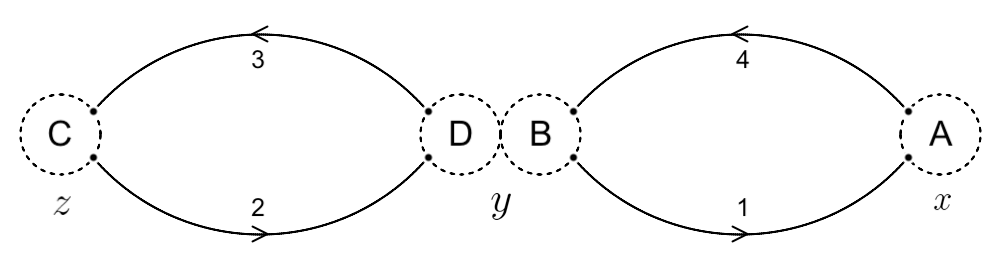
\includegraphics[width=0.8\textwidth]{imgs-MSc-thesis/Wick_stochastic_disc.png}
    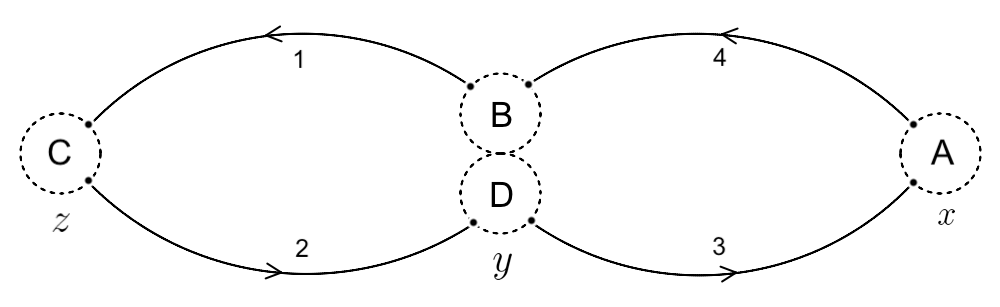
\includegraphics[width=0.75\textwidth]{imgs-MSc-thesis/Wick_stochastic_conn.png}
    \caption{On the top: graph of disconnected Wick contraction. On the bottom: graph of connected Wick contraction. The variables are such that $x_4 > y_4 > z_4$.}
\end{figure}\label{fig:contractions-stochastic-method}
\newline
After Wick contractions, the correlators read:
\begin{equation}\label{eq:contractions-stochastic-method}
    \begin{gathered}
        G_d = \sum_{\vec x, \vec y, \vec z} \bigg\langle \text{Tr}\left[\Gamma_A S_{(3,+)}(x,y)\Gamma_B S_{(4,+)}(y,x)\right]\cdot\text{Tr}\left[\Gamma_C S_{(1,+)}(z,y)\Gamma_D S_{(2,+)}(y,z)\right] \bigg\rangle^{\text{sea}} \\
        G_c = - \sum_{\vec x, \vec y, \vec z} \bigg\langle \text{Tr}\left[\Gamma_A S_{(3,+)}(x,y)\Gamma_D S_{(2,+)}(y,z)\Gamma_C S_{(1,+)}(z,y)\Gamma_B S_{(4,+)}(y,x)\right] \bigg\rangle^{\text{sea}}
    \end{gathered}
\end{equation}
\newline
I generate $N_{\text{noise}}$ stochastic spinors in the timeslice $x_0$ and $N_{\text{noise}}$ stochastic spinors in the timeslice $z_0$.
I refer to the formers with $\eta^{1}$ and the latters with $\eta^{2}$.
These stochastic spinors have again a Dirac index ($\alpha,\beta,\cdots$) and a colour index ($a,b,\cdots$).
The properties (\ref{eq:eta-properties}) must be generalized to:
\begin{equation}
    \begin{gathered}
        \langle \eta^{1}_{a\alpha} (u) \rangle^{\text{noise}} = \langle \eta^{2}_{b\beta} (u) \rangle^{\text{noise}} = 0 \\
        \langle \eta^{1*}_{a\alpha} (u) \eta^{2}_{b\beta} (v) \rangle^{\text{noise}} = \langle \eta^{2*}_{a\alpha} (u) \eta^{1}_{b\beta} (v) \rangle^{\text{noise}} = 0 \\
        \langle \eta^{1*}_{a\alpha} (u) \eta^{1}_{b\beta} (v) \rangle^{\text{noise}} = \delta_{a,b} \delta_{\alpha,\beta} \delta_{\vec u, \vec v} \delta_{u_0,x_0} \delta_{v_0,x_0} \\
        \langle \eta^{2*}_{a\alpha} (u) \eta^{2}_{b\beta} (v) \rangle^{\text{noise}} = \delta_{a,b} \delta_{\alpha,\beta} \delta_{\vec u, \vec v} \delta_{u_0,z_0} \delta_{v_0,z_0} \\
    \end{gathered}
\end{equation}
I define the following derived stochastic spinors:
\begin{equation}
    \begin{aligned}
        & \zeta^{(i,\pm)}_{j} (u) = \sum_{v} S_{(i,\pm)}(u,v)\eta^{j}(v) \\
        & \xi^{(i,\pm)}_{j,X} (u) = \sum_{v} S_{(i,\pm)}(u,v) \gamma_5 \Gamma_X^\dag \eta^{j}(v)
    \end{aligned}
\end{equation}
It could be easily checked that the contractions in (\ref{eq:contractions-stochastic-method}) are obtained by the following formulae:
\begin{equation}\label{eq:noise-method}
    \begin{gathered}
        G_d =   \sum_{\vec y} \left\langle \left\langle \left(\gamma_5\xi^{(3,-)}_{1,A} (y) \right)^\dag \Gamma_B \zeta^{(4,+)}_1 (y) \cdot \left(\gamma_5\xi^{(1,-)}_{C,2} (y) \right)^\dag \Gamma_D \zeta^{(2,+)}_2 (y) \right\rangle^\text{noise} \right\rangle^{\text{sea}} \\
        G_c = - \sum_{\vec y} \left\langle \left\langle \left(\gamma_5\xi^{(3,-)}_{1,A} (y) \right)^\dag \Gamma_D \zeta^{(2,+)}_2 (y) \cdot \left(\gamma_5\xi^{(1,-)}_{C,2} (y) \right)^\dag \Gamma_B \zeta^{(4,+)}_1 (y) \right\rangle^\text{noise} \right\rangle^{\text{sea}}
    \end{gathered}
\end{equation}
Then, to evaluate the previous couple of Wick contraction I need only four quantities for each couple of stochastic spinors:
\begin{equation*}
    \xi^{(3,-)}_{1,A} (y) \qquad  \zeta^{(4,+)}_1 (y) \qquad \xi^{(1,-)}_{C,2} (y) \qquad  \zeta^{(2,+)}_2 (y)
\end{equation*}
To summarize, the path to evaluate the correlators is:
\begin{itemize}
    \item [$\triangleright$] For each Gauge-sea configuration evaluate 2$N_{\text{noise}}$ spinors - $N_{\text{noise}}$ for $\eta^1$ and $N_{\text{noise}}$ for $\eta^2$. 
    \item [$\triangleright$] For each noise spinor evaluate the quantities $\zeta^{(i,\pm)}_j$ and $\xi^{(i,\pm)}_{j,X}$ needed.
    \item [$\triangleright$] Evaluate the correlators and evaluate the noise average.
    \item [$\triangleright$] Iterate the procedure and calculate the sea average.
    \item [$\triangleright$] At the end, the simulation program gives back the correlator $G_d+G_c$.
\end{itemize}
Let's look at the {\bf computational advantage}.
Each time I compute the quantities $\xi^{(i,\pm)}_{j,X}$ of $\zeta^{(i,\pm)}_j$ I'm {\it not} evaluating the inverse of a matrix in $\text{Mat}(N\x N, \mathbb{R})$, but its inverse on a vector of length $N$.
Then the needed computational resources are decreased and the simulation algorithms result improved.
Furthermore, I need ``only'' $4\cdot N_\text{noise} \cdot N_\text{noise} \cdot N_\text{configurations} $ inversion of this kind for each three points correlator.
Then, for a reasonable choise of $N_\text{noise}$, the advantage is succesfully achieved\footnote{in practice, almost always.}.

\section{Simulation program description}\label{sec:program}
\noindent
The program is structured to generate three points correlation functions and it is based on a previous version that calculates meson propagators.
It makes use of modules from \texttt{OpenQCD-1.2}\footnote{\href{https://luscher.web.cern.ch/luscher/openQCD/index.html}{https://luscher.web.cern.ch/luscher/openQCD/index.html}}, allowing calculations with open boundary conditions.
The program takes in input an ensemble of sea configurations and produces the correlators of the form (\ref{eq:lattice-correlators}) with $x_4, z_4$ fixed and $y_4$ running in the time region $[z_4,x_4]$.
Instead of read some external configurations, it is also possible to set the link variables to identity $U_\mu(x) = \mathbb{I}_3$ (absence of interactions, because $A_\mu^{i} \hspace*{.1mm}_j = 0$) or to randomly generate them.
These two options were very useful to test the correct behaviour of the simulation.
The program requires the following input parameters:
\begin{itemize}
    \item [-] The coefficient of the Sheikholeslami-Wohlert term $c_{SW}$ and $c_F$, another coefficient for the boundary counterterms of the fermionic action.
                The latter is set to $c_F = 1$.
    \item [-] Informations about the noise spinor method: the number of noise vectors $N_\text{noise}$ per set and the generating distibution chosen from one of the following $U(1)$, \texttt{Gauss}, $\mathbb{Z}_2$.
    \item [-] Quark flavours informations: the critical mass $M^i_\text{cr}$ and the bare twisted mass parameter $\mu_i$ for each quark.
    \item [-] Dirac matrices: $\Gamma_\omega$, $\Gamma_\xi$ for the source bilinears and $\Gamma_\sigma$, $\Gamma_\rho$ for the intermediate operator.
        The program allows to insert different operators within the same sources and calculate their Wick contractions.
        It is also possible to choose which quark to insert in each propagator.
\end{itemize}
At the end the program stores output data in a file written in \texttt{LITTLE\_ENDIAN} or \texttt{BIG\_ENDIAN} depending on the machine used.
The output data are already summed over all the spatial components.

\subsection{Computational Basis}
\noindent
One might wonder the reason behind the choice of exchange operators $\Gamma_B \leftrightarrow \Gamma_D$ between the terms $G_d$ and $G_c$ of the previous method (look at equations (\ref{eq:GdGc-strategy})).
It could seem an unreasonable choice because it has the form of a flavour exchange $(1\leftrightarrow 3)$ instead of $(2\leftrightarrow 4)$, that one might expect.
Behind this choice lies a subtlety developed for computational convenience.
\newline
I can rewrite the set of operators $\{O_{i,[+]}^\text{tw}\}$ in equations (\ref{eq:O_i-operators-twisted-final}) in the following compact forms:
\begin{equation}
    \begin{split}
        & O_{1[+]}^\text{tw} = \mp 2i \left( V^{12}A^{34} + A^{12}V^{34} + V^{14}A^{32} + A^{14}V^{32} \right) \\
        & O_{2[+]}^\text{tw} = \mp 2i \left( V^{12}A^{34} - A^{12}V^{34} - V^{14}A^{32} + A^{14}V^{32} \right) \\
        & O_{3[+]}^\text{tw} = \pm 2i \left( P^{12}S^{34} - S^{12}P^{34} - P^{14}S^{32} + S^{14}P^{32} \right) \\
        & O_{4[+]}^\text{tw} = \pm 2i \left( P^{12}S^{34} + S^{12}P^{34} + P^{14}S^{32} + S^{14}P^{32} \right) \\
        & O_{5[+]}^\text{tw} = \pm 2i \left( \tilde{T}^{12}T^{34} + T^{14}\tilde{T}^{32} \right) \\
    \end{split}
\end{equation}
Clarifications about the notation can be found in Appendix \ref{app:notations}.
I want to group togheter the minimal elements to compute the $C_i^\text{FR}$s in a simulation.
This strategy brought me to redefine again - and for the last time - the operators.
They read:
\begin{equation*}
    \begin{split}
        & \Psi_{1} =  V^{12}A^{34} + A^{14}V^{32} \hspace*{40pt} O_{1[+]}^\text{tw} = \mp 2i \left( \Psi_{1} + \Psi_{2} \right) \\
        & \Psi_{2} =  A^{12}V^{34} + V^{14}A^{32} \hspace*{40pt} O_{2[+]}^\text{tw} = \mp 2i \left( \Psi_{1} - \Psi_{2} \right) \\
        & \Psi_{3} =  P^{12}S^{34} + S^{14}P^{32} \hspace*{40pt} O_{3[+]}^\text{tw} = \pm 2i \left( \Psi_{3} - \Psi_{4} \right) \\
        & \Psi_{4} =  S^{12}P^{34} + P^{14}S^{32} \hspace*{40pt} O_{4[+]}^\text{tw} = \pm 2i \left( \Psi_{3} + \Psi_{4} \right) \\
        & \Psi_{5} =  \tilde{T}^{12}T^{34} + T^{14}\tilde{T}^{32} \hspace*{40pt} O_{5[+]}^\text{tw} = \pm 2i \cdot \Psi_{5} \\
    \end{split}
\end{equation*}
As usual, through them I recover the operators $O_{i,[+]}^\text{tw}$.
Each of the new operators has the form:
$$\Psi_i = \bar\psi_1 \Gamma_D \psi_2 \cdot \bar\psi_3 \Gamma_B \psi_4 + \bar\psi_1 \Gamma_B \psi_4 \cdot \bar\psi_3 \Gamma_D \psi_2$$
that {\it is} a flavour exchange $1 \leftrightarrow 3$ and {\it not} $2 \leftrightarrow 4$.
Thus I directly evaluate this kind of correlator $\forall i$:
$$\bigg\langle \bar K'^0(x) \Psi_i (y) \bar K^0(z) \bigg\rangle \sim \bigg\langle \left(\bar\psi_4 \Gamma_A \psi_3 \right) (x) \Psi_i (y) \left(\bar\psi_2 \Gamma_C \psi_1 \right) (z) \bigg\rangle$$
and it can be verified that it gives exactly the contractions $G_c + G_d$ of Figure \ref{fig:contractions-stochastic-method}.
With the symbol $\sim$ I refer to the fact that the two correlators have the same structure, i.e. they are {\it similar} from a computational point of view.
Then the output data of simulation program has no physical meaning until I perform the basis change in data analysis time.\footnote{To be precise, the physical meaning is achieved only in the continuum limit $a \rightarrow 0$.}

\section{Analysis strategy}\label{sec:analysis}
\noindent
This section provides an overview of the analysis strategy needed to recover the lattice bag parameters $\mathcal{B}_i (a)$ through the method based on asymptotic behaviours outlined in section \ref{sec:asympt-behav}.
Once recovered the $\mathcal{B}_i (a)$s at different values of lattice spacing $a$, the continuum limit $a\rightarrow 0$ will give the best estimate of the physical parameters $B_i$.
The analysis is divided in some steps, that I report below.
This analysis strategy holds for all the data generated from gauge configurations with open boundary conditions, involving CLS ensembles.

\subsubsection*{First step: determination of minimal ``asymptotic distance'' $\delta_4$}
\noindent
In order to perform the calculation in (\ref{eq:bag-parameters-extraction}):
\begin{equation*}
    \begin{gathered}
        \mathcal{B}_1 (a;y_4) = \frac{1}{\xi_1} \cdot \frac{C_1^\text{FR}(x_4,y_4,z_4)}{X^\text{FR}_{34}(x_4,y_4)\cdot X^\text{FR}_{12}(y_4,z_4)} \\
        \mathcal{B}_i (a;y_4) = \frac{1}{\xi_i} \sum_{j} \Lambda_{ij} \frac{C_i^\text{FR}(x_4,y_4,z_4)}{G^\text{FR}_{34}(x_4,y_4)\cdot G^\text{FR}_{12}(y_4,z_4)}
    \end{gathered}
\end{equation*}
I need the values of such two points and three points correlators in the temporal regions in which the asymptotic behaviour of Section \ref{sec:asympt-behav} is allowed.
In other words, I need to quantify the minimum value of $\delta_4 = |x_4-y_4|$ such that the exponentials $e^{-\delta_4 m_i}$ - for $m_i > m_K$ - are {\it sufficiently} suppressed with respect to the first level contribution $e^{-\delta_4 m_K}$.
To estimate it, I make use of two points correlators $G_{12}^\text{FR}(y_4,z_4)$ and $G_{34}^\text{FR}(x_4, y_4)$, namely the mesons propagators.
Let's start with the first.
From the proof \ref{app:sinh-proof} I know that, in the asymptotic regime $y_4 \gg z_4$\footnote{In the paper \cite{OBC-tm} by Luscher it is not given the complete result, but only the last $y_4$ dependence. A proof of the complete result is a personal achievement reported in the Appendix \ref{app:proofs}.}:
\begin{equation}\label{eq:sinh}
    G_{12}^\text{FR}(y_4,z_4) \approx \frac{\sinh \left( m_K (T - y_4) \right) \cdot \sinh \left( m_K z_4 \right)}{2 m_K \sinh \left( m_K T \right)} \propto \sinh \left( m_K (T - y_4) \right)
\end{equation}
In the last equality I fixed $z_4 = a$, choice valid in the entire simulation.
I fix $z_4 = a$ and run the simulation for all the $y_4 \in (z_4+a,T-a)$.
The case $y_4 = T$ will not produce physical results because of open boundary conditions on fermion fields.
The strategy consists in performing a fit of the hyperbolic sine in different regions of the space.
I start to fit in the maximal region $[a, T-a]$ and decrease it step by step $[2a,T-2a], [3a,T-3a], \dots $ until the goodness of the fit reaches a satisfactory previously chosen value.
Up to now, no such goodness parameters has been chosen.
The first satisfactory region gives the value of $\delta_4$: $[\delta_4, T-\delta_4]$.
At this point I will have determined both $m_K$ as a parameter and the ``minimal asymptotic distance'' $\delta_4$.
In this region I also have the values of $G_{12}^\text{FR}(y_4,z_4=a) = \hat G_{12}^\text{FR}(y_4,a)$ subject to a well defined asymptotic expansion.
I denote them with the {\it hat} identifier to stress that these data are the ones to be used to recover the wanted quantities.
\newline
Then the same procedure must be done for the other two points correlator, $G_{34}^\text{FR}(x_4, y_4)$.
In this case $x_4$ must be intended as fixed to $T-a$, while $y_4 < x_4$ varies.
In this case the complete formula of the correlator is again (\ref{eq:sinh}), but the fit must be on the second variable:
\begin{equation*}
    G_{34}^\text{FR}(x_4, y_4) \propto \sinh \left( m_{K'} y_4 \right)
\end{equation*}
By repeating the previous analysis, one should get a value of $m_{K'}$ and a data set of correlators $G^\text{FR}_{34}(x_4=T-a,y_4) = \hat G^\text{FR}_{34}(T-a,y_4)$ useful for the next setps.
Moreover there comes another value of minimal asymptotic distance $\delta_4'$.
I simply chose to use the larger of the two, that I call again $\delta_4$.
\newline
With $x_4$ and $z_4$ fixed I will take, by varying $y_4$, the data to be used in (\ref{eq:bag-parameters-extraction}),
namely $\hat X_{12}^\text{FR}(y_4,a)$ with $y_4 - a > \delta_4$ and $\hat X_{34}^\text{FR}(T-1,y_4)$ with $ T-a - y_4 > \delta_4$.

\subsubsection*{Second step: recovering lattice bag parameters $\mathcal{B}_i$}
\noindent
At this point I will be ready to analyze three points correlators $C_i^\text{FR}(x_4,y_4,z_4)$.
I take a set of correlators with $z_4 = a$, $x_4 = T-a$ while $y_4$ varies in $(z_4,x_4)$.
I expect to see a plateaux region for $C_i^\text{FR}$ in $y_4 \in (z_4 + \delta_4 , x_4 - \delta_4)$ because I know from the analysis of $G^\text{FR}_{12,34}$ that the higher mass states are already suppressed.
Thus the only relevant contribution comes from lattice Kaons.
In such region I rename them $\hat C_i^\text{FR}(x_4,y_4,z_4)$.
\newline
The results of previous steps are used to recover values of the $\mathcal{B}_i (a)$ for a given set of Gauge configuration, i.e. for a given value of lattice spacing $a$:
\begin{equation*}
    \mathcal{B}_i (a;y_4) = \frac{1}{\xi_i} \sum_{j=1}^5 \Lambda_{ij} \mathcal{F}_j (a;y_4)
\end{equation*}
I have different values of $\mathcal{B}_i$ corresponding to different choices of $y_4$.
It is possible that some {\it residues} of higher mass states contribution are still present.
A fit on a plateaux region of the graph $\mathcal{A}_i (a) (y_4)$ vs $y_4$ will help to remove them.
I expect to see that plateaux region for values of the euclidean time $y_4$ much larger than $z_4$ and sufficiently smaller than $x_4$.
At this point, I will have extracted the best estimate for the lattice bag parameters $\mathcal{B}_i (a)$.

\subsubsection*{Third step: continuum limit extrapolation of $B_i\bare$}
\noindent
A set of configurations it is always generated by setting some parameters, for example the inverse of coupling constant $g$.
By analyzing some observables of the gauge fields it is possible to recover the value of the lattice spacing $a$ associated to an ensemble of configurations.
\newline
Repeating the previous analysis for different sets of gauge ensembles brings to a set of parameters for different values of the lattice spacing $\mathcal{B}_i (a_1), \mathcal{B}_i (a_2), \dots$.
The essential step to get the {\it physical} values of the bag parameters $B_i$ is the continuum limit extrapolation.
It consists in:
$(i)$ a fit of lattice values versus their associated lattice spacing that gives the function $\mathcal{B}_i^\text{fit} (a) $ and
$(ii)$ an \oaid\space extrapolation of the physical values through $ B_i = \mathcal{B}_i^\text{fit} (0) + O(a^2)$.

\section{Status of the work, results and future developments}\label{sec:status}
\noindent
In this section I outline the status of this work and possible future developments.
The program behaviour has been tested both in the vacuum $U_\mu (x) = \mathbb{I}_3$ $\forall \mu,x$ and through unphysical random configurations.
The relevant tests reported consist into two checks of gauge invariance of two and three points correlators.
Gauge invariance is an essential property of QFTs; for this reason it is one of the most checked in lattice QCD simualtions.
Then the program has been tested on two ensembles of quenched\footnote{i.e. in absence of sea quarks, neglecting the fermion determinant in (\ref{eq:fermion-determinant}).} gauge fields with OBC.
\newline
The first test furnishes a direct proof that the Dirac inverter preserves gauge invariance property.
Unwanted errors could be found from a lack in this test.
A set of pointlike spinors has been generated.
I define {\it pointlike} spinor an $\eta$ defined by:
$$\eta_\alpha^a (x) = \delta^{a,\bar a}\delta_{\alpha, \bar \alpha} \delta_{x,\bar x}$$
with $\bar a, \bar \alpha, \bar x$ fixed colour, Dirac and lattice indices.
This has been done for all the $3\times 4 = 12$ combinations of fixed Dirac and colour indices, meanwhile $\bar x$ was kept unchanged.
By inverting the Osterwalder-Seiler operator on them, the propagators were expected to have this structure:
\begin{equation*}
    \left(S^{(f)}(y, \bar x)[U]\right)^{b,\bar a}_{\beta, \bar \alpha} \hspace*{1cm} \forall \hspace*{0.3mm} b,\beta,y
\end{equation*}
with $f$ the flavour index.
I have explicitly contracted propagators and Dirac matrices to reconstruct Wick contractions of previous chapter.
This has been made by fixing two pointlike sources $\bar x=(\vec 0, x_4)$ and  $\bar z=(\vec 0, z_4)$, by choosing a mixing operator $\Psi_i (y)$ and summing over the fixed colour and Dirac indices.
In other words, the {\it noise average} in formula (\ref{eq:noise-method}) is replaced by the sum over two sets of 12 pointlike sources.
In both tests the values of $z_4$ and $x_4$ were fixed respectively to the first and last allowed timeslice.
This has been done for random sea fields and their gauge transformed fields.
The propagators are expected to transform in the following way:
\begin{equation*}
    \left(S^{(f)}(y, \bar x)[\Omega U \Omega^\dagger]\right)^{b,\bar a}_{\beta, \bar \alpha} = \Omega (y)^{b,c} \left(S^{(f)}(y, \bar x)[U]\right)^{c,d}_{\beta, \bar \alpha} \Omega^\dagger (\bar x)^{d,\bar a}
\end{equation*}
thus the traces appearing in the Wick contractions (\ref{eq:wick-contractions-general}) are gauge invariant.
The check of gauge invariance has been succesfully achieved by comparing two set of data of three points correlators obtained using a (random) configuration and its gauge transformed duplicate.
The gauge transformations $\Omega (x)$ were randomly generated.
Figure \ref{fig:check1} shows the output of the described test, in which the intermediate operator is $\Psi_3 (y)$.
Since the three points correlators are real, only the real part is plotted.
Such reality property is proven in \ref{app:proof-reality-3pts}.
\begin{figure}[h!]
    \centering
    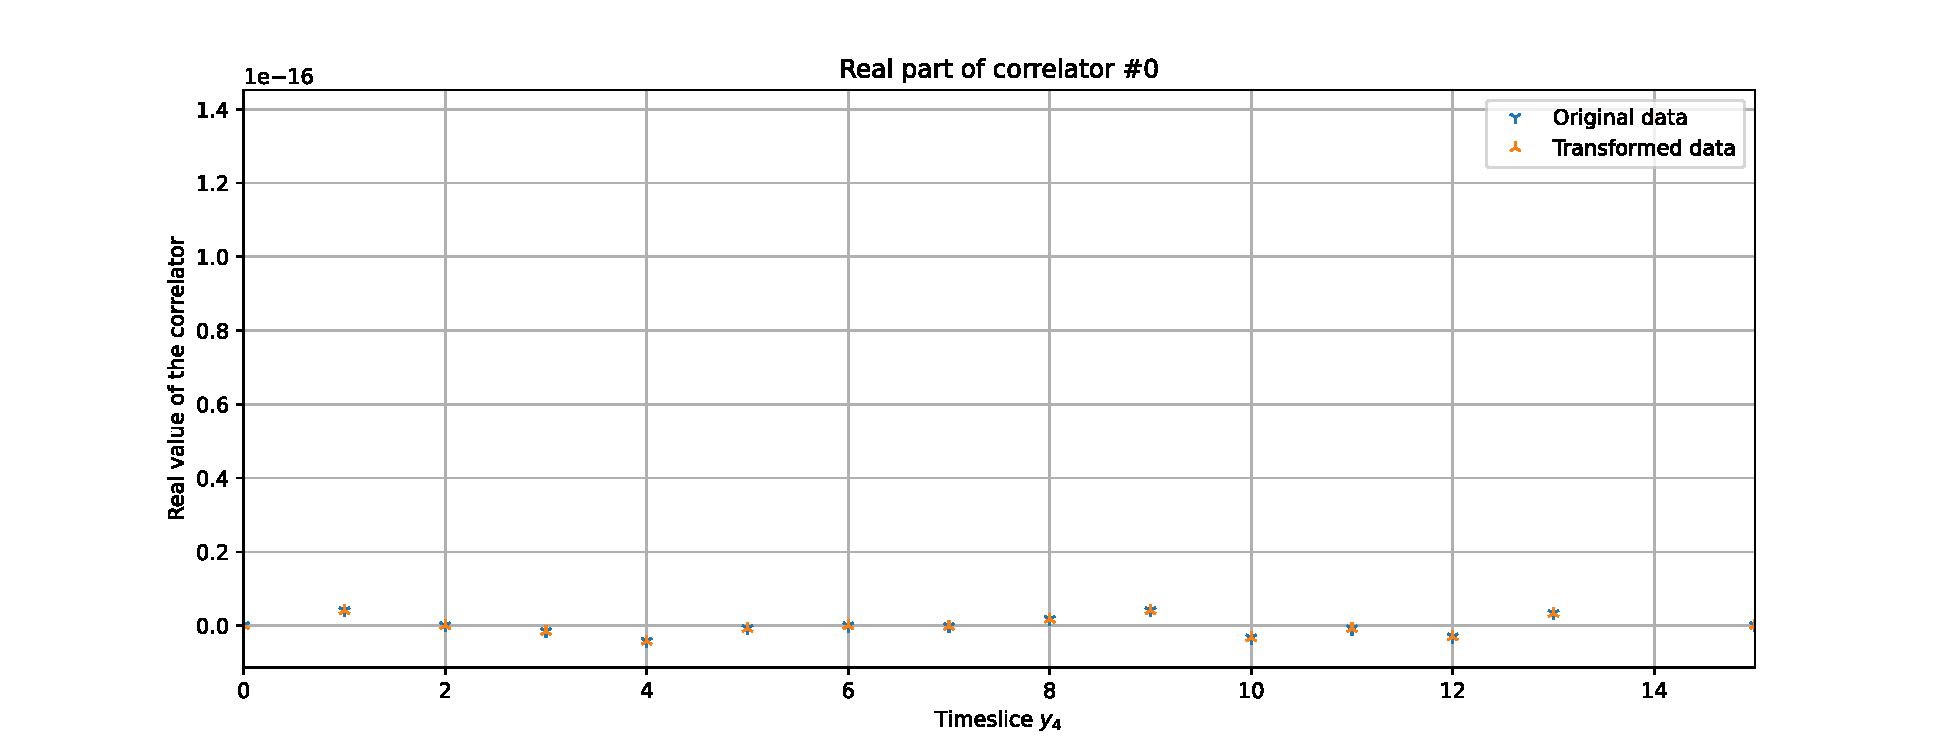
\includegraphics[width=\textwidth]{imgs-MSc-thesis/check1.pdf}
    \caption{Check of Gauge invariance on the 3 points correlators.
        The plot shows the three point correlator $\sum_{\vec y} \la \bar K^{0'} (14a) \Psi_3 (y_4, \vec y) \bar K^0 (a) \ra$ versus the timeslice $y_4$.
        The gauge fields are randomly generated, the sources are a $\gamma_5$ and an $\mathbb{I}_4$ to emulate Kaon sources in OS twist.
        The point in $y_4=1$ is out of range, but exhibits the same gauge invariance property.
        I stress that these data are not physically meaningful.}
    \label{fig:check1}
\end{figure}
\newline
In both the tests the finite precision of the solver generates discrepancies between the two data sets, but they are visible only at scales much smaller than the correlators scale.
It has been verified that these errors decrease requiring more and more precision in the inversion of the propagators.
Moreover all the physical parameters were not well tuned, since they were not useful to the scope of the checks. 
\newline
The second test aims to verify gauge invariance of the three points correlators calculated through the noise spinors method, equation (\ref{eq:noise-method}).
It consists in the following steps.
First of all, it has been generated a set of random unphysical link variables $U_\mu (x)$ and they were used to compute correlators through formula (\ref{eq:noise-method}).
Then data were stored and analyzed.
The second part consisted in the generation of random gauge transformations $\Omega (x)$.
The previous gauge configuration has been transformed and it followed a re-computation of the correlators.
The two data sets must coincide up to errors.
This test served to quantify the minimum number of noise spinors $N_\text{noise}$ to make the stochastic method effective.
To better understand it, a set of graphs in Figure \ref{fig:check2} shows the plots of such test using respectively $N_\text{noise} = 5,20,50,100$ noise spinors.
\begin{figure}[h!]
    \centering
    \begin{subfigure}[b]{0.49\textwidth}
        \centering
        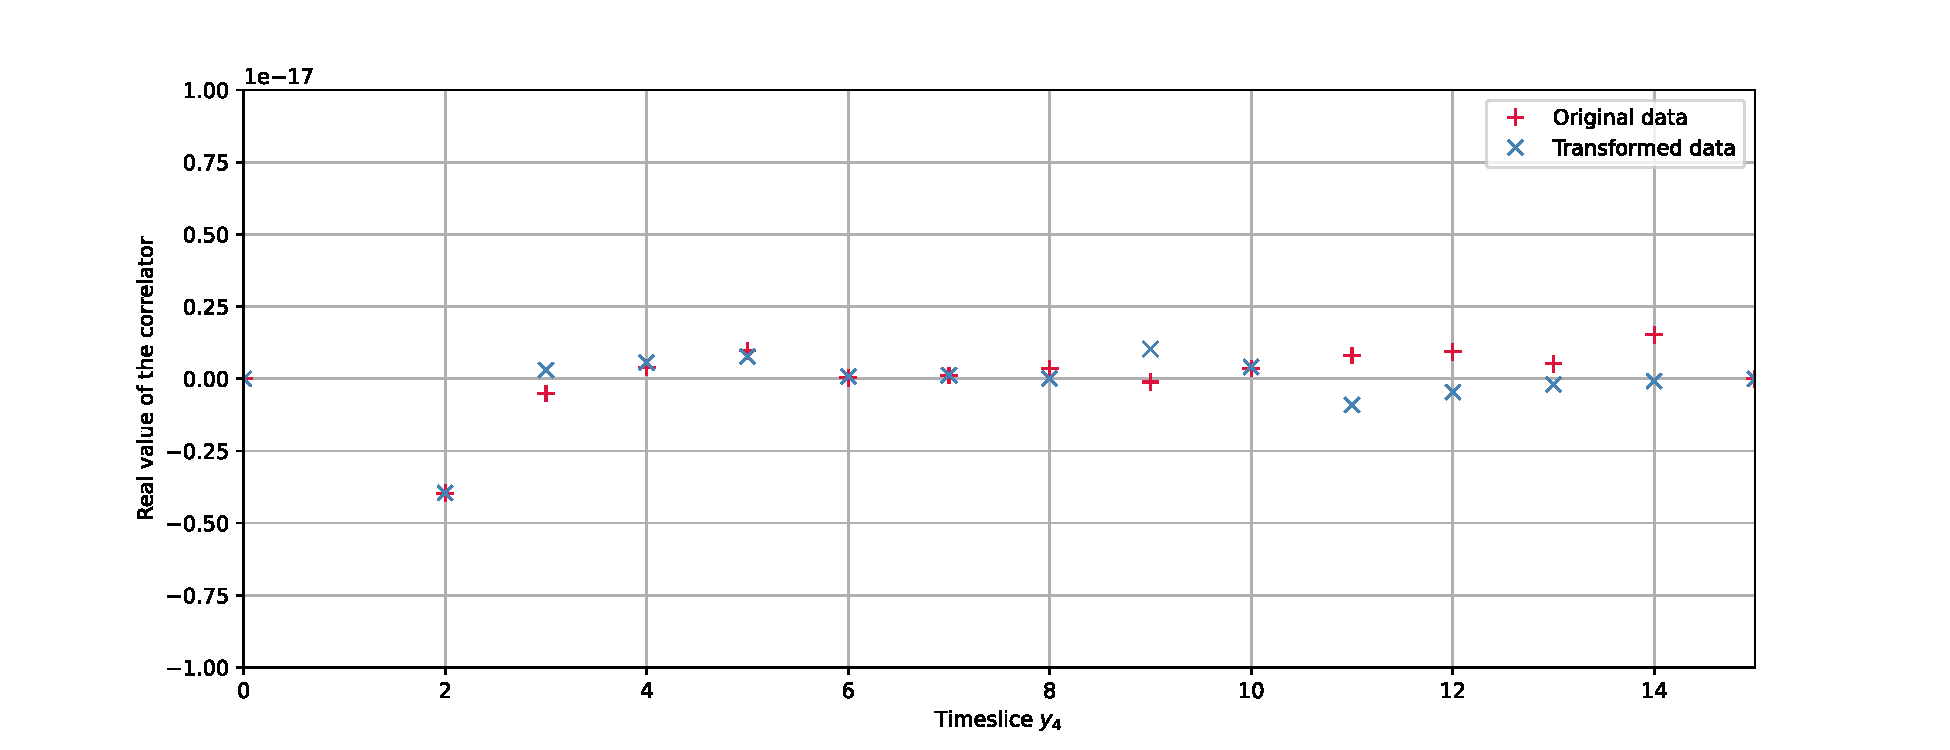
\includegraphics[width=\textwidth]{imgs-MSc-thesis/check2-5.pdf}
        \caption{$N_\text{noise}=5$}
    \end{subfigure}
    \begin{subfigure}[b]{0.49\textwidth}
        \centering
        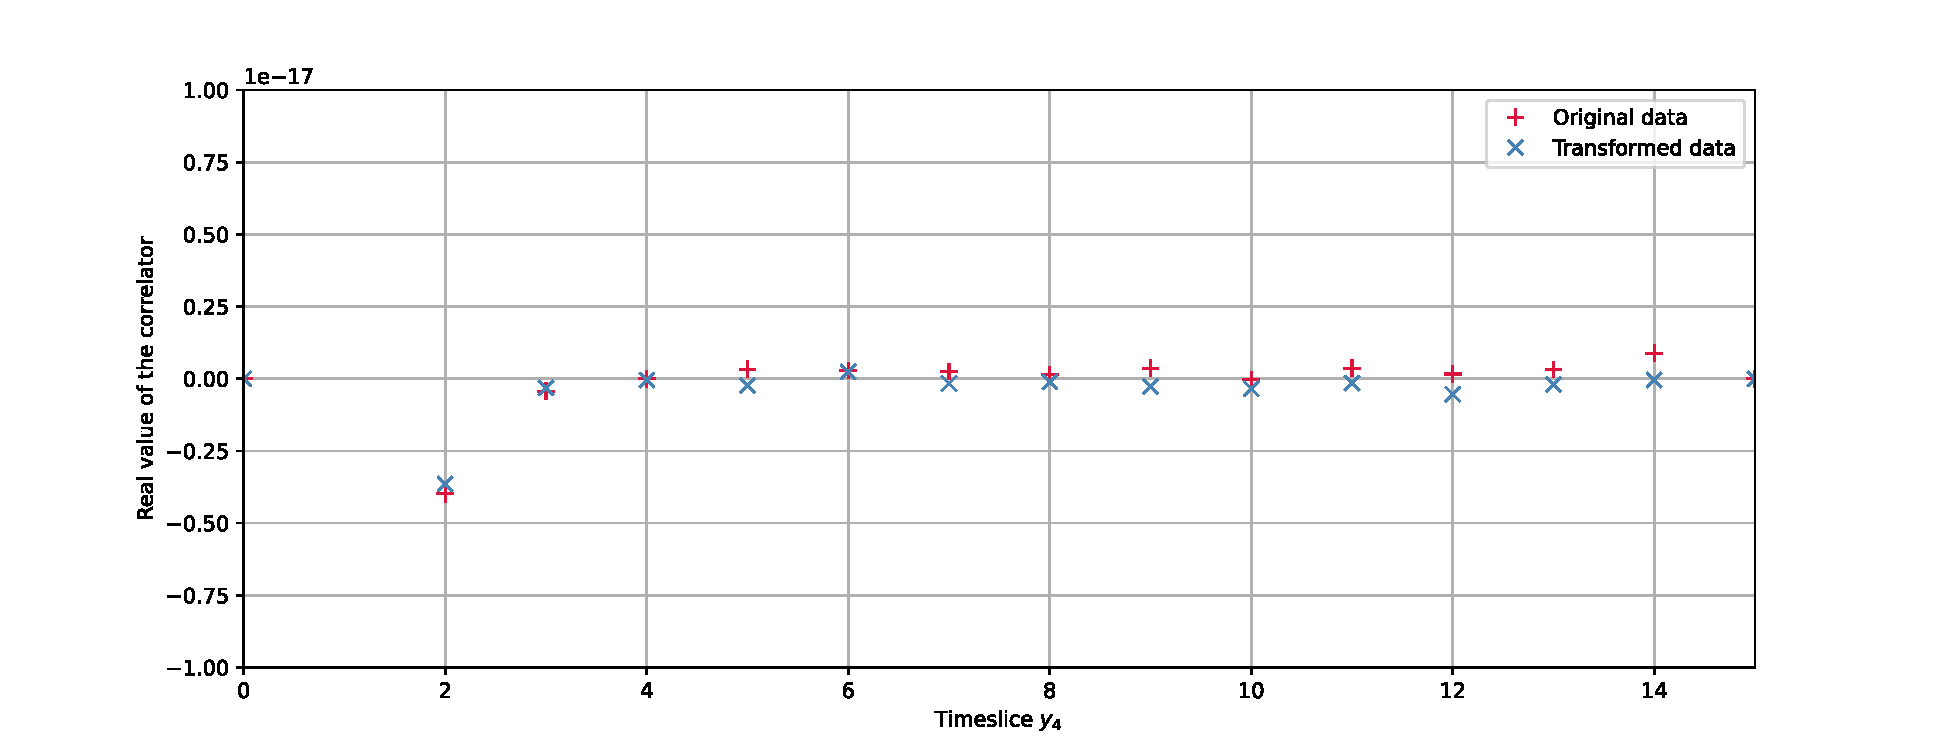
\includegraphics[width=\textwidth]{imgs-MSc-thesis/check2-20.pdf}
        \caption{$N_\text{noise}=20$}
    \end{subfigure}
    \begin{subfigure}[b]{0.49\textwidth}
        \centering
        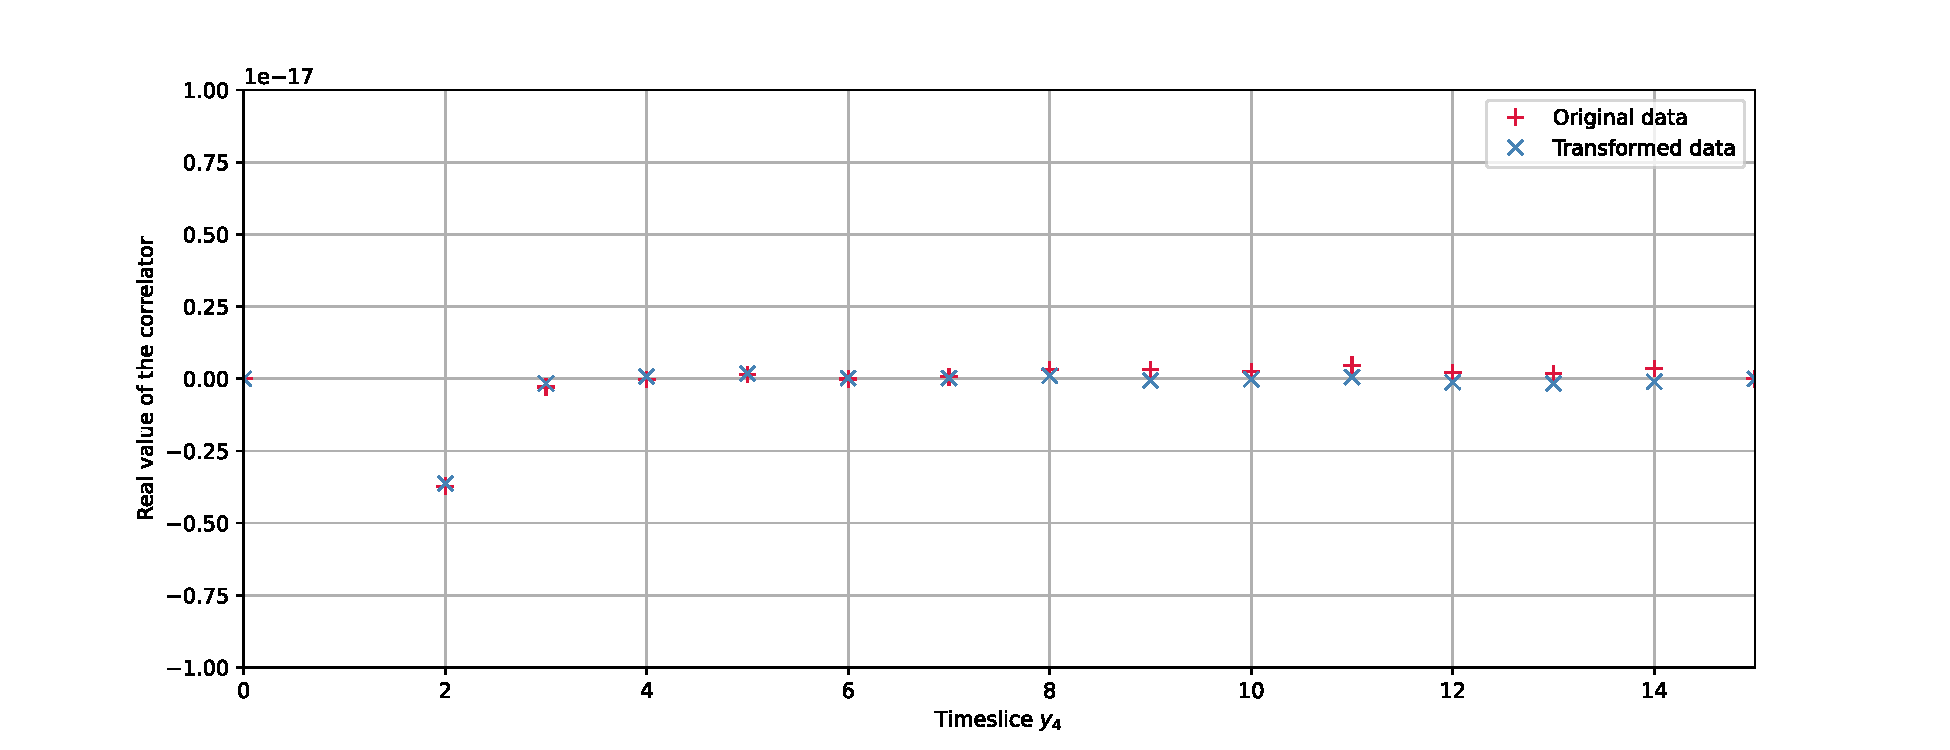
\includegraphics[width=\textwidth]{imgs-MSc-thesis/check2-50.pdf}
        \caption{$N_\text{noise}=50$}
    \end{subfigure}
    \begin{subfigure}[b]{0.49\textwidth}
        \centering
        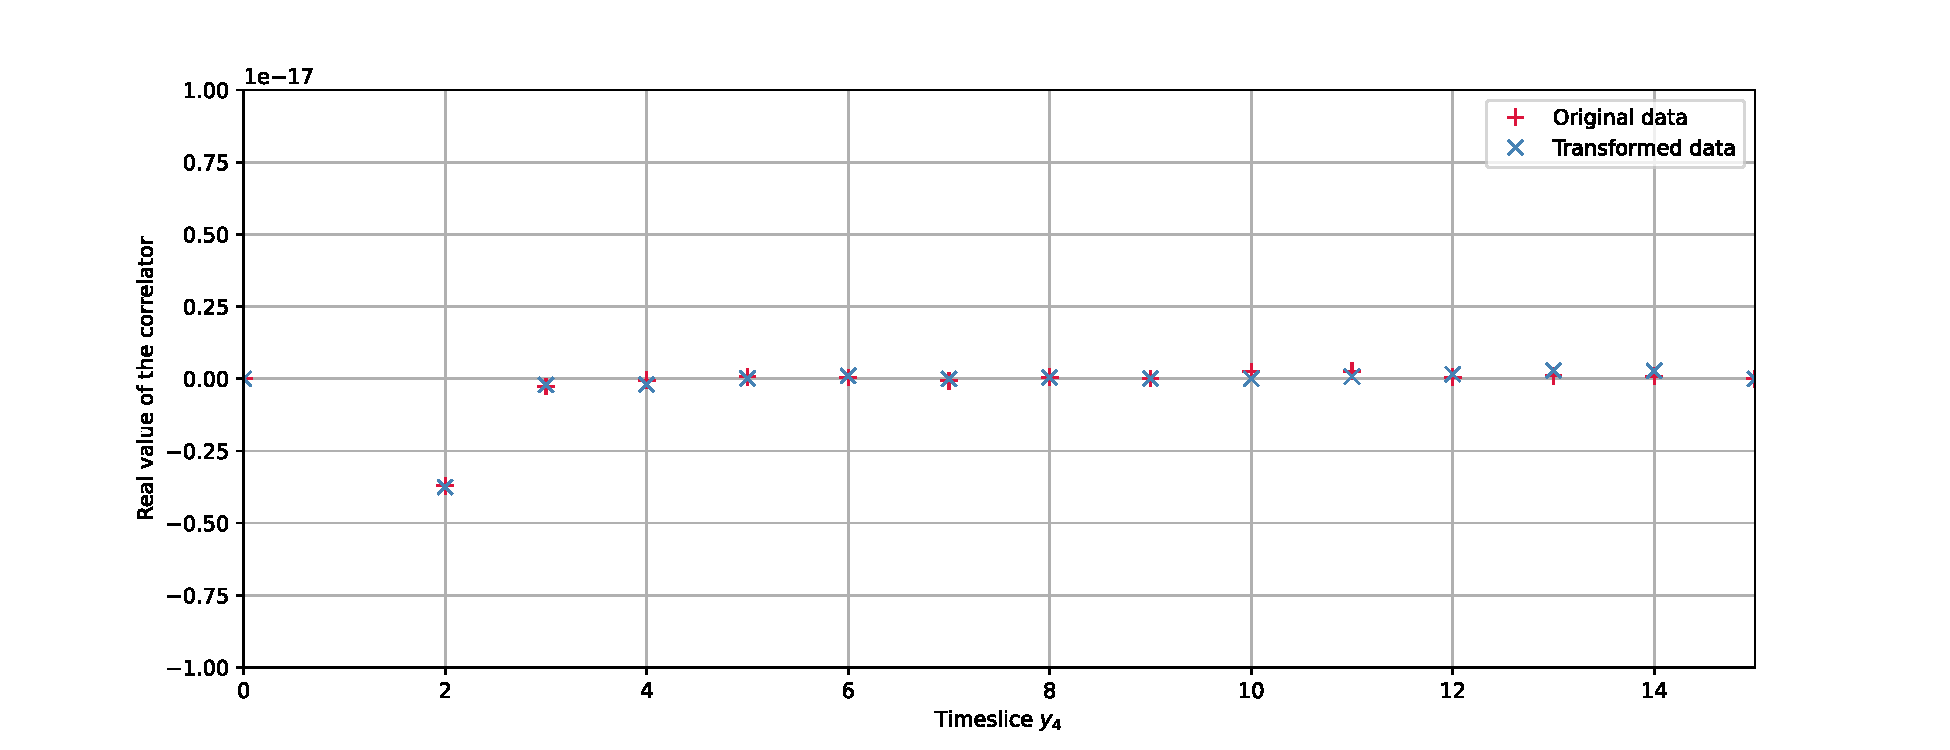
\includegraphics[width=\textwidth]{imgs-MSc-thesis/check2-100.pdf}
        \caption{$N_\text{noise}=100$}
    \end{subfigure}
    \caption{Second gauge invariance test executed on random link variables. Such $U_\mu(x)$ are the same for each of the four tests.
        The plots show the real part of the integrated correlator $\sum_{\vec y} \la \bar K^{0'} (14a) \Psi_3 (y_4, \vec y) \bar K^0 (a) \ra$ for different values of $N_\text{noise}$.
        The distibution served to extract the random $\eta^i$ is $U(1)$.}
    \label{fig:check2}
\end{figure}
In order to quantify the error due to different number of stochastic sources, I introduced the following estimator:
\begin{equation*}
    \varepsilon(N_\text{noise}) = \frac{1}{N_T-2}\sum_{y_4}\left(\frac{|C(y_4)-\tilde C(y_4)|}{C(y_4)+\tilde C(y_4)}\right)
\end{equation*}
The values of such estimator for different choices of number of stochastic sources are listed in Table \ref{tab:estimator}.
The values seems to be rapidly decreasing for $N_\text{noise} \lesssim 35$ while stabilizing for $N_\text{noise} \gtrsim 35$.
To complete the study of the numebr of noise spinors through this estimator, a set of $\varepsilon$s for a large amount of configurations should be tested.
\begin{table}[h!]
    \centering
    \begin{tabular}{|c||c|c|c|c|c|c|}
        \hline
        $N_\text{noise}$ & 5 & 20 & 35 & 50 & 70 & 100 \\
        \hline
        $\varepsilon$ & 2.140 & 2.598 & 1.350 & 1.342 & 1.243 & 0.533 \\ 
        \hline
  \end{tabular}
  \vspace*{3mm}
  \caption{Values of the estimator $\varepsilon$ for different values of $N_\text{noise}$ from a single simulation.}
  \label{tab:estimator}
\end{table}
\newline
Another test has been done on an ensemble of 54 gauge configurations generated using the \texttt{OpenQCD-1.2} program.
The gauge configurations have been generated with and inverse lattice coupling $\beta = 6/g_0^2 = 6.0$ - corresponding to an inverse lattice spacing $a^{-1} \sim 2.0$ \gev \cite{exploring-tmQCD-clover-term} - in the quenched approximation.
The value of the coefficient $c_0$ in equation (\ref{eq:gaugeaction-LuscherWeisz}) is set to $5/3$, then the simulated action is the {\it tree level Symanzik improved}.
The lattice has dimension \texttt{16x16x16x32}, where 32 is the number of points in time direction.
First of all the configurations have been tested on the program that calculates two points correlators.
The simulation involved $N_\text{noise} = 30$ noise spinors and the hopping parameters used were not at their critical value, thus the maximal twist is not achieved.
Despite this, the simulation furnishes a test on the two point functions behaviour.
The correspondig graph, in logarithmic scale, is presented in Figure \ref{fig:plot-2pts}.
\begin{figure}[!h]
    \centering
    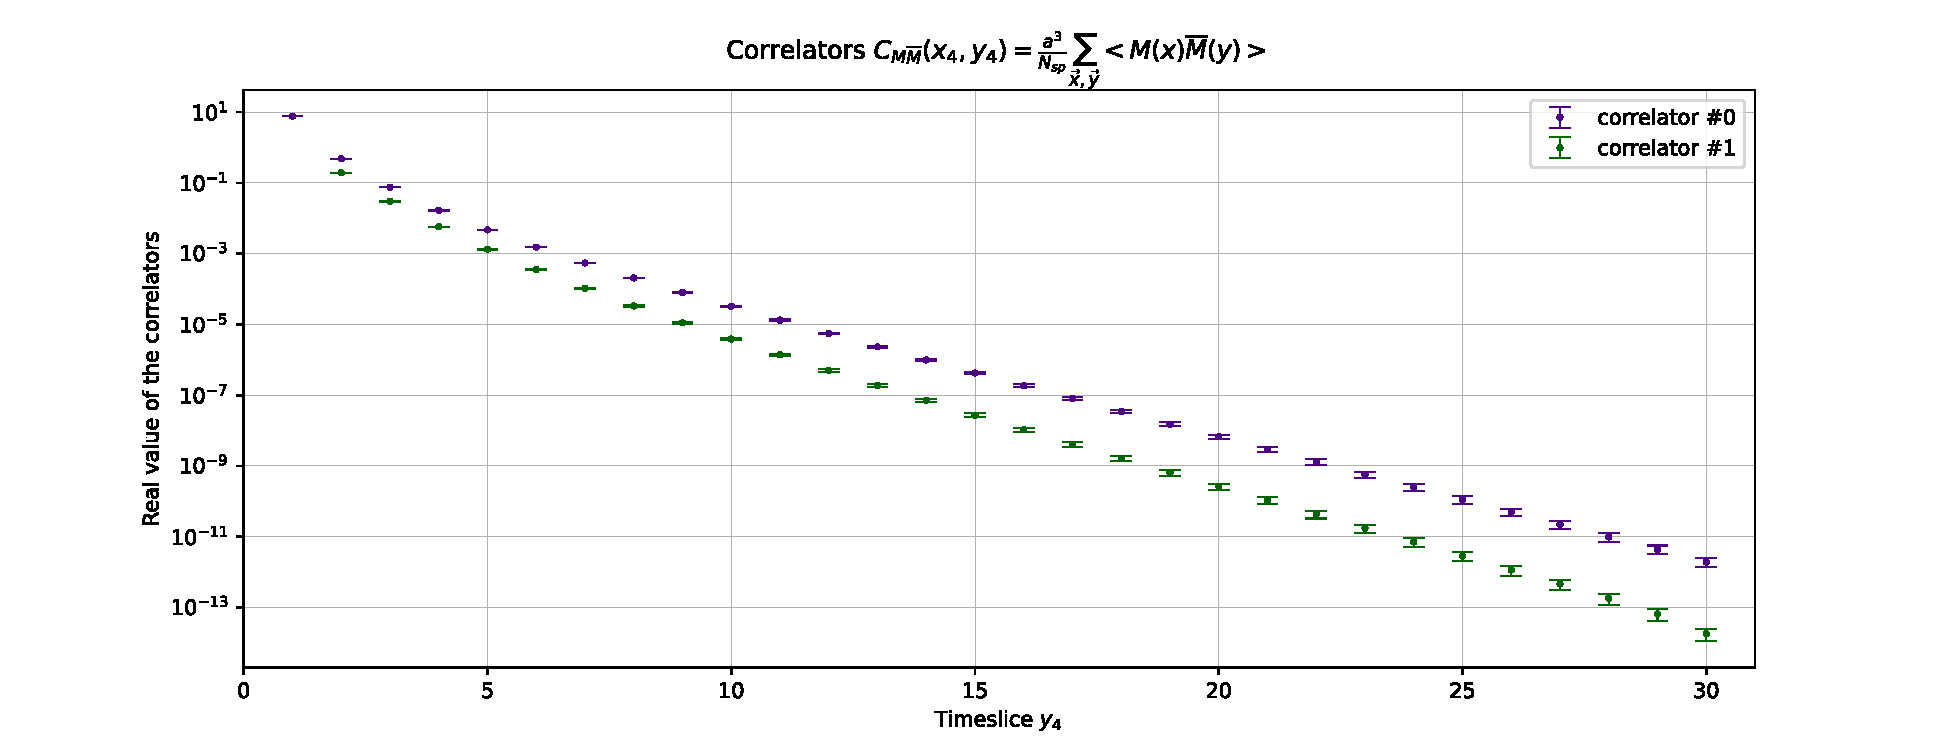
\includegraphics[width=\textwidth]{imgs-MSc-thesis/pureYM-2pts.pdf}
    \caption{Two points correlators $\sum_{\vec x, \vec y} \la \bar K^0 (y) K^0 (x) \ra$ and $\sum_{\vec x, \vec y} \la \bar K^{0'} (y) K^{0'} (x) \ra$.
        Test executed with hopping parameters different from the critical value and twisted mass terms different from zero.}
    \label{fig:plot-2pts}
\end{figure}
Here $x_4<y_4$ with fixed $x_4=a$.
The behaviour of the two point correlators is, as expected, similar to the one in Figure 6 in \cite{OBC-tm}.
Such behaviour is proportional to:
\begin{equation*}
    \propto C + \log\big[\sinh \left(M_i (T-y_4)\right)\cdot \sinh \left(M_i x_4\right)\big] = C' + M_i \left(T+x_4-y_4\right) + \log \left[f(x_4,y_4)\right]
\end{equation*}
that's a line plus a logarithm of a function $f$ of the time coordinates.
The two points correlators considered are the scalar and pseudoscalar propagators, i.e. $G_{12}^\text{FR}(y_4,x_4)$ and $G_{34}^\text{FR}(y_4,x_4)$.
\newline
Then the case of three points correlators is inspected.
The correlators were calculated through $N_\text{nosie} = 20$ noise spinors and the Figure \ref{fig:pureYM} shows the results.
\begin{figure}[!h]
    \centering
    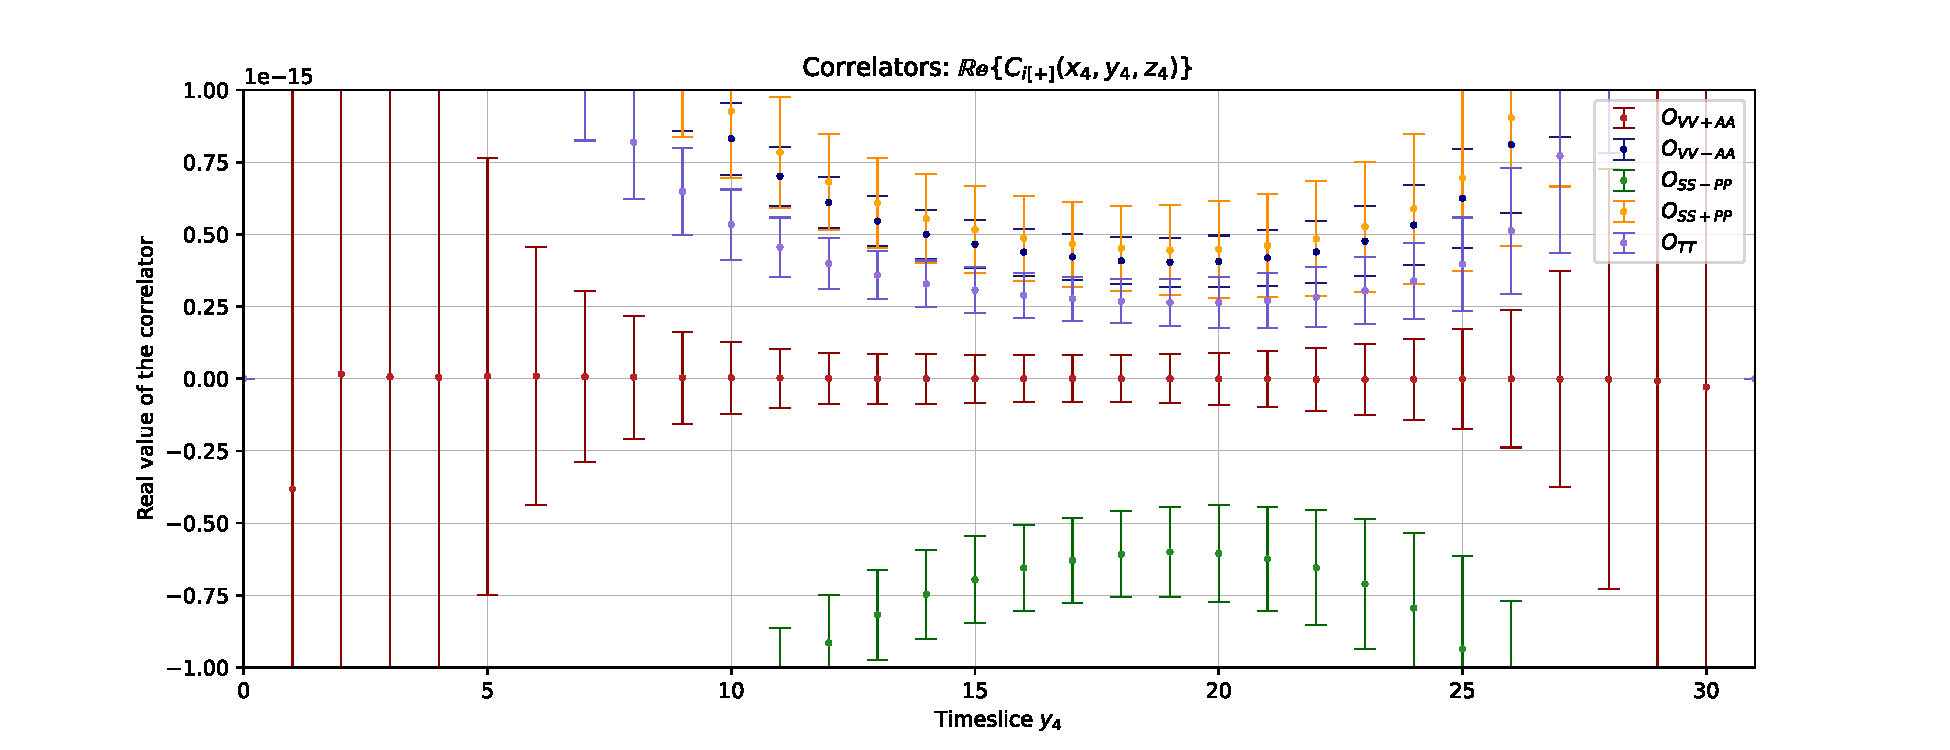
\includegraphics[width=\textwidth]{imgs-MSc-thesis/pureYM-3pts.pdf}
    \caption{Test of the simulation program on 54 quenched configurations on a \texttt{16x16x16x32} lattice, $\beta = 6.0$, tree level improved Symanzik gauge action.}
    \label{fig:pureYM}
\end{figure}
\newline
Clearly the plot is not at all satisfactory because there are no plateaux regions.
On the other hand, the fermion physical parameters had no physical meaning because their determination requires a lot of work, not necessary for a simple test such that.
Then the maximal twist is not achieved and such correlators are meaningless.
Usually the physical parameters, such as $K_\text{crit}$ and $\mu_i$s, are given along with the configuration, when available and already been studied.
Moreover the first correlator has values extremely small - by one order or more - compared to values from the other operators.
The immaginary part of these correlators have been plotted and the plot confirms that these correlators are real.
The plot is reported in Appendix \ref{app:proof-reality-3pts}.
\newline
The last test of the simulation program was made on 37 gauge configurations in quenched approximation.
They are generated through \texttt{OpenQCD-1.2} program, with $\beta=6.0$ and $c_0 = 1.0$ and a \texttt{16x16x16x32} lattice.
These parameters are chosen to simulate the plaquette Guage action.
The reason behind this choice relies in the results of paper \cite{exploring-tmQCD-clover-term}.
In such paper the critical hopping parameter of twisted fermions has been studied for such configurations and the most precise result gives $K_\text{crit} = 0.135217$.
This results has been used to simulate three points correlators, along with other parameters:
\begin{itemize}
    \item [-] down quark twisted mass: $a|\mu_d| = 0.0038$.
    \item [-] strange quark twisted mass used is: $a\mu_s = 0.1482$.
    \item [-] the coefficient of Sheikholeslami-Wohlert term is set to $c_{SW}=1.769$, from \cite{Luscher-cSW}.
\end{itemize}
Due to the use of $K_\text{crit}$, the maximal twist is achieved.
The plot of the integrated correlators $C_i^\text{FR}$ are shown in Figure \ref{fig:plaq-ym} below:
\begin{figure}[!h]
    \centering
    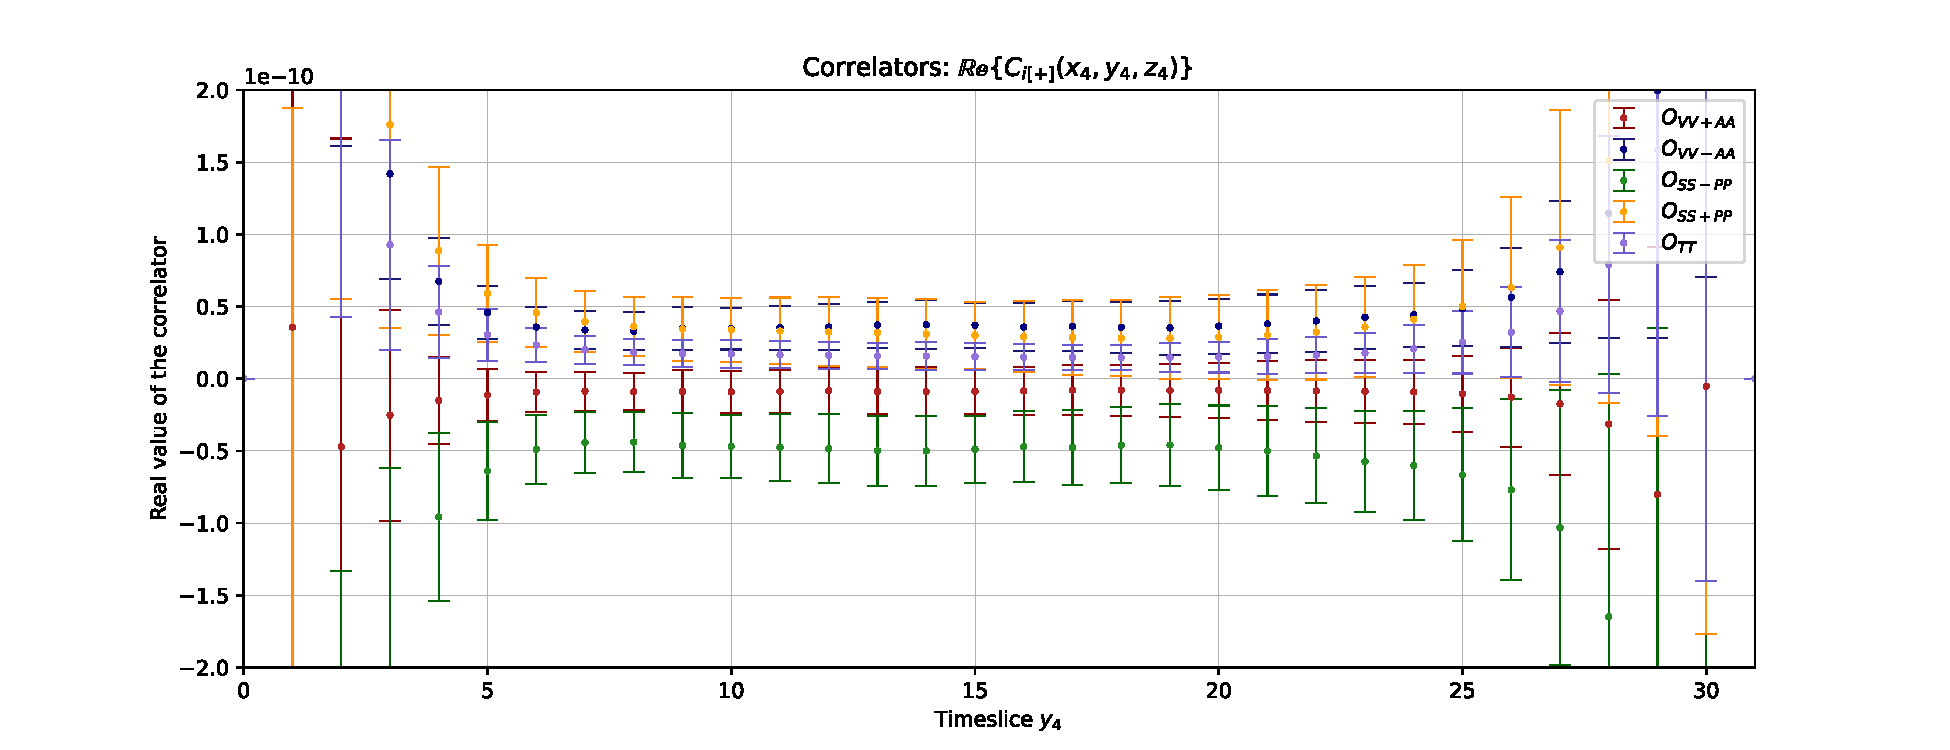
\includegraphics[width=\textwidth]{imgs-MSc-thesis/plaqAct-3pts.pdf}
    \caption{Test of the simulation program on 37 quenched configurations on a \texttt{16x16x16x32} lattice, $\beta = 6.0$, plaquette action.}
    \label{fig:plaq-ym}
\end{figure}
\newline
As can be seen, the good choice of fermion parameters associated to the configurations generated more evident plateaux regions.
Large error bars are due to the small number of noise sources and the small number of configurations analyzed.
Moreover the first operator does not exhibit a null plateaux, unlike what is shown in Figure \ref{fig:pureYM}.
\newline
The results of $C_i^\text{FR}$ are used to recover the lattice ratios:
\begin{equation*}
    \mathcal{R}_i (a;y_4) = \sum_{j=2}^5 \Lambda_{ij} \frac{C_j^\text{FR}(T-a,y_4,a)}{C_1^\text{FR}(T-a,y_4,a)}
\end{equation*}
Because of lack of large number of data, statistics results too low to determine a plateaux region with satisfactory precision.
\begin{figure}[!h]
    \centering
    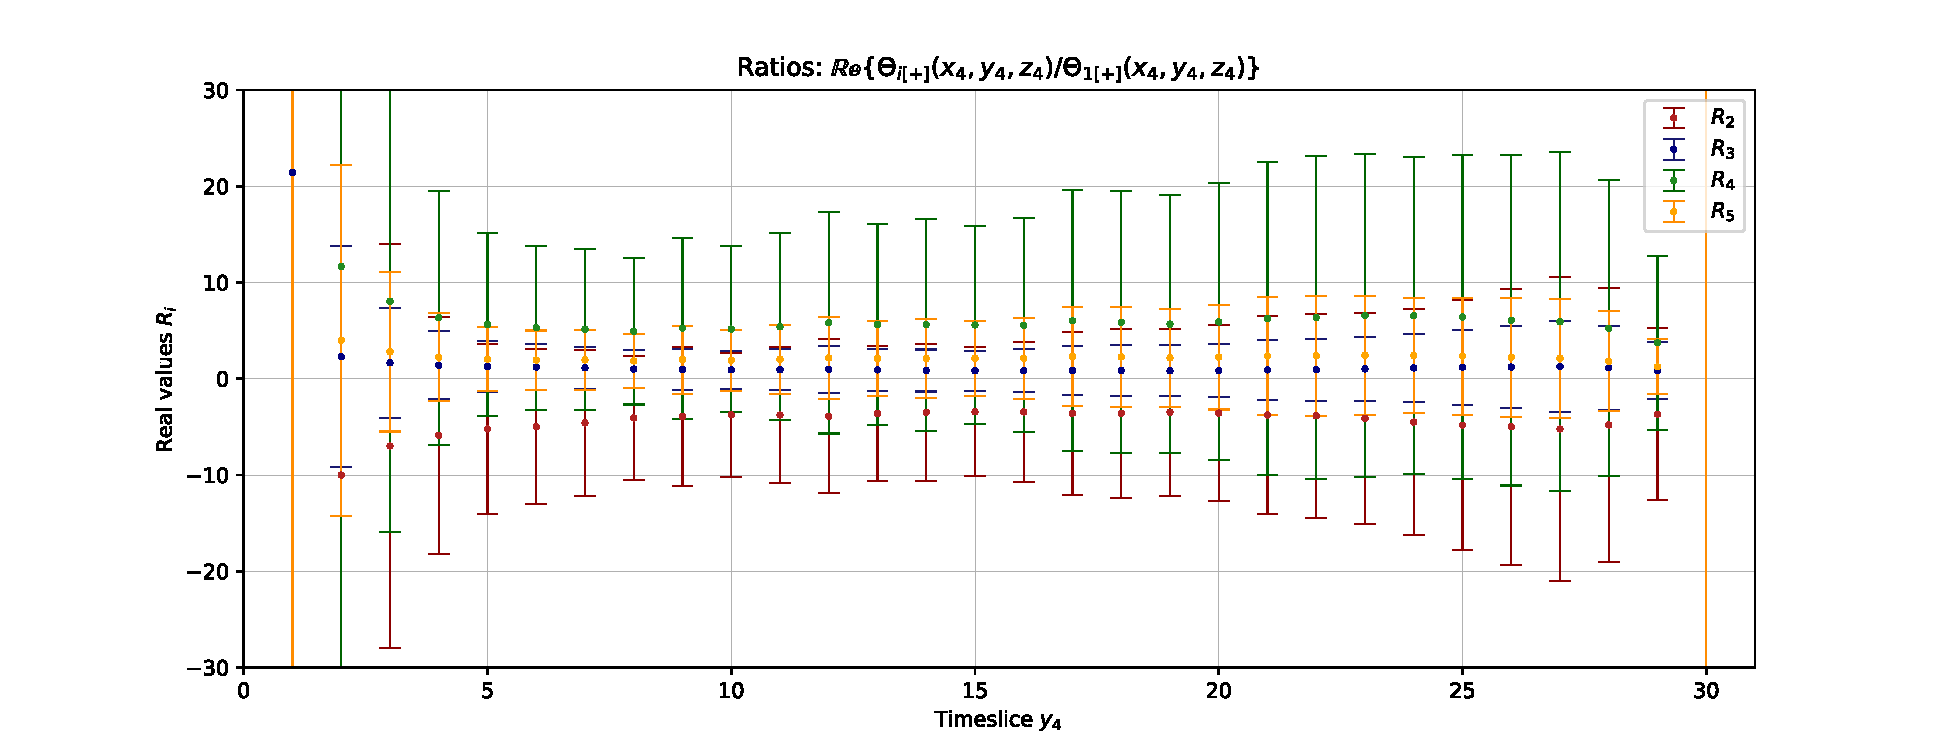
\includegraphics[width=\textwidth]{imgs-MSc-thesis/ratios.pdf}
    \caption{Ratios $\mathcal{R}_i (a;y_4)$ with lattice spacing $a\sim (2 \text{ Gev})^{-1}$ on the last set of gauge configurations.}
    \label{fig:ratios}
\end{figure}

\subsubsection*{Future developments}
\noindent
Future developments involve the calculation of three points correlators by using faithful sea configurations and tuning the fermion parameters.
The purpose is to do that using the Coordinated Lattice Simulations\footnote{Coordinated Lattice Simulations: \href{https://wiki-zeuthen.desy.de/CLS/}{https://wiki-zeuthen.desy.de/CLS/}}, generated through the \texttt{open-QCD}\footnote{Open-QCD packages: \href{https://luscher.web.cern.ch/luscher/openQCD/index.html}{https://luscher.web.cern.ch/luscher/openQCD/index.html}} (CLS) ensembles \cite{Bruno} with $N_f = 2+1$ improved sea quarks.
These configurations have been studied in a wide licterature of works\footnote{For some examples, consult Bibliography at the end of the thesis.} and contains $N_f = 2+1$ quarks in the sea.
On these ensembles the fermion parameters are well tuned through complex and precise procedures \cite{Bruno} \cite{obc-opt3}.
The two points meson correlators are studied, for example in \cite{LightMesons}.
To do that, a match between sea quarks masses and valence masses is required, as done in \cite{matching-masses}.
The results of bare bag parameters $B_i$ on CLS configurations will be a cutting edge result.


%%%APPENDICE%%%
\appendix %Da questo comando in poi si hanno capitoli non numerati impostati come "appendice" anziché "capitolo"

\chapter{Notations and conventions}\label{app:notations}
\noindent
The metric employed in this study is the Euclidean metric $g_{\mu\nu} = \delta_{\mu\nu}$.
In this context, there is no differentiation between upper and lower Dirac indices.
I usually prefer to use lower indices.
\newline\newline
The Dirac matrices employed belong to the so-called ``chiral representation'' \cite{Itzykson-Zuber}.
Dirac matrices and Lorentz generators for spinors are as follows:
\begin{equation*}
    \begin{gathered}
        \gamma_i = \sigma_2 \otimes \sigma_i \qquad \gamma_0 = - \sigma_1 \otimes \mathbb{I}_2 = -\gamma_4 \\
        \gamma_5 = \gamma_0 \gamma_1 \gamma_2 \gamma_3 = \sigma_3 \otimes \mathbb{I}_2 \\
        \qquad \text{properties } \left\{ \gamma_\mu , \gamma_\nu \right\} = 2 \delta_{\mu\nu} \mathbf{I}_4 \text{ and } \left\{ \gamma_\mu , \gamma_5 \right\} = 0 \\
        \sigma_{\mu\nu} = \frac{i}{2} \left[\gamma_\mu , \gamma_\nu\right] = i \left(\gamma_\mu \gamma_\nu - \delta_{\mu\nu} \mathbf{I}_4\right) \\
        \tilde{\sigma}_{\mu\nu} = \frac{1}{2}\epsilon_{\mu\nu\rho\omega}\sigma_{\rho\omega} = \gamma_5 \sigma_{\mu\nu} 
    \end{gathered}
\end{equation*}
The Lagrangian densities in Minkowski and Euclidean spaces are:
\begin{equation*}
    \begin{gathered}
        \mathcal{L}_M = - \bar{\psi} \left( \gamma_\mu \left( \partial_\mu + i A_\mu \right) + m \right) \psi \\
        \mathcal{L}_E = \bar{\psi} \left( \gamma_\mu \left( \partial_\mu + i A_\mu \right) + m \right) \psi
    \end{gathered}
\end{equation*}
This leads to the Dirac equation and its Dirac conjugate (valid in both Minkowski and Euclidean metrics):
\begin{equation*}
    \begin{gathered}
        \left( \gamma_\mu \left( \partial_\mu + i A_\mu \right) + m \right) \psi = 0 \\
        \bar{\psi} \left( \gamma_\mu \left( \partial_\mu + i A_\mu \right) - m \right) = 0
    \end{gathered}
\end{equation*}
Dirac bilinears are typically expressed in the following form: $\bar \psi^1 \Gamma^\alpha \psi^2$ with $\psi^1$ and $\psi^2$ representing two distinct flavours.
The Dirac operators belong to this set:
\begin{equation*}
    \Gamma^{\alpha} \in \{\mathbb{I}_4,\gamma_\mu, \gamma_5, \gamma_\mu\gamma_5, \sigma_{\mu\nu}, \tilde\sigma_{\mu\nu} \}
\end{equation*}
and a shorthand notation is $X^{12} = \bar \psi^1 \Gamma^\alpha \psi^2$ where $X = S, V, P, A, T, \tilde{T}$ indicates which matrix is chosen.
For example $V^{12}A^{34} = \bar \psi^1 \gamma_\mu \psi^2 \bar \psi^3 \gamma_\mu \gamma_5 \psi^4$.
\newline
\newline
A very useful property \cite{Itzykson-Zuber} follows:
\begin{equation}\label{eq:complconj-bilinear}
    \begin{aligned}
        & \left( \bar\psi^1 \Gamma^\alpha \psi^2 \right)^* = \left( \bar\psi^1 \Gamma^\alpha \psi^2 \right)^\dag = -\bar\psi^2 \bar \Gamma^\alpha \psi^1 \\
        & \text{with } \bar \Gamma^\alpha = \gamma_0 \Gamma^{\alpha,\dag} \gamma_0.
    \end{aligned}
\end{equation}
for example in the case of Kaons $\left(K^0\right)^* = \bar K^0$.

\chapter{Twisted basis vs physical basis}\label{app:physical-basis}

\section{Twisted and physical basis in tmQCD}
\noindent
In the context of twisted mass lattice QCD described in \ref{sec:tmLQCD}, it is possible to define a physical fermion basis as follows:
\begin{equation*}
    \chi = \mathbf{T}(\alpha)\hspace*{0.5mm} \psi \hspace*{1cm} \overline{\chi} = \bar\psi\hspace*{0.5mm}\mathbf{T}(\alpha)
\end{equation*}
Here, $\mathbf{T}(\alpha)$ represents the twist rotation (\ref{eq:twist}).
In this scenario, the twisted mass action takes the following form:
\begin{equation}\label{eq:physical-action}
    S^\text{phys}_\text{tm} [\chi,\overline{\chi},U] = a^4 \sum_{x,y} \overline{\chi} (x) \left( D_{xy}^\text{tm} + M_q \mathbb{I}_2 \delta_{xy}\right) \chi (y)
\end{equation}
where the new bilinear operator is given by:
\begin{equation*}
    D^\text{tm}_{xy} = -\frac{1}{2a} \sum_{\mu = \pm 1}^{\pm 4} \left[ (\mathbf{T}(-2\alpha) - \gamma_\mu) U_\mu (x) \delta_{x+\hat\mu,y} \right] +\frac{4}{a} \hspace*{0.5mm} \mathbf{T}(-2\alpha)
\end{equation*}
The key steps to establish this are:
\begin{enumerate}
    \item Recall the properties $(\gamma_5)^2=\mathbb{I}_4$ and $(\sigma^3)^2=\mathbb{I}_2$
    \item Expand the exponential: $\mathbf{T}(\alpha) = \cos(\alpha/2)\mathbb{I}_4\otimes\mathbb{I}_2 + i\sin(\alpha/2)\gamma_5\otimes\sigma^3$
    \item Use the Clifford algebra $\{\gamma_\mu,\gamma_\nu\}= 2\delta_{\mu\nu}\mathbb{I}_4$ and Lie algebra of $SU(2)$ $[\sigma^a,\sigma^b]=2i\epsilon^{abc}\sigma^c$ to modify the Wilson-Dirac operator $D_{xy} \mapsto D_{xy}^\text{tm}$
\end{enumerate}
The new set of variables $\{\chi,\bar\chi\}$ is referred to as the {\it physical} basis because it doesn't involve the (unphysical) term $\mu_q$.
In other words, the mass is entirely transformed and encapsulated in $M_q = \sqrt{m^2+\mu_q^2}$.
The twist rotation modifies the Wilson term, which undergoes modification. 
Despite this, it is known \cite{montvay-munster} that the Wilson term vanishes in the continuum limit.
Consequently, the action (\ref{eq:physical-action}) tends towards the physical continuum action.
Thus, it represents the ``true'' discretization of the continuum theory, while the twisted action defined in (\ref{eq:tmQCD-action}) is the modified action.
\newline
The link between the two actions lies in the twist rotation of fermion fields.
I will demonstrate that an expectation value can be computed in both theories.
It's important to keep in mind that the framework in which the theory is applied is the functional integral formalism, so we must pay attention to the integration measure.
The variable change:
\begin{equation*}
    \mathcal{D}\chi \hspace*{0.5mm} \mathcal{D}\overline{\chi} \mapsto \mathcal{D}\psi \hspace*{0.5mm} \mathcal{D}\overline{\psi}
\end{equation*}
it is not anomalous\footnote{i.e. it does not introduce measure anomalies}.
Moreover, the Jacobian is a constant $\mathbf{T}^2(\alpha)$.
Since a constant doesn't affect the observables expectation values, I state - with abuse of this term - that the Jacobian is the identity.
Next, I present the main result of this section: for a field-dependent observable $\mathcal{X}$, its expected value in both formulations coincides:
\begin{equation*}
    \la \mathcal{X} [\chi, \overline{\chi}, U] \ra_{(M_q,0)} = \la \mathcal{X}' [\psi, \overline{\psi}, U] \ra_{(m,\mu_q)}
\end{equation*}
with $\mathcal{X}' [\psi, \overline{\psi}, U] = \mathcal{X} [\mathbf{T}(\alpha)\psi, \overline{\psi}\mathbf{T}(\alpha), U]$.
The power of tmQCD theory lies in this substitution of variables.
\newline
Now, I provide a list of some straightforward operators - currents and densities - along with their transformation rules.
First of all I define four quantities:
\begin{itemize}
    \item [] $\qquad$ Scalar density: \hspace*{5mm} $S^{0,\text{phys}} = \bar\chi \chi$
    \item [] $\qquad$ Pseudoscalarcalar densities: \hspace*{5mm} $P^{a,\text{phys}} = \bar\chi \gamma_5 \frac{\sigma^a}{2} \chi$
    \item [] $\qquad$ Vector currents: \hspace*{5mm} $V_{\mu}^{a,\text{phys}} = \bar\chi \gamma_\mu \frac{\sigma^a}{2} \chi$
    \item [] $\qquad$ Axial vector currents: \hspace*{5mm} $A_\mu^{a,\text{phys}} = \bar\chi \gamma_\mu \gamma_5 \frac{\sigma^a}{2} \chi$
\end{itemize}
where the superscript ``phys'' refers to the physical basis $\{\chi,\bar\chi\}$.
Analogous definitions hold for the basis $\{\psi,\bar\psi\}$.
I apply a twist $\mathbf{T}(\alpha)$ to get the twisted operators:
\begin{itemize}
    \item [] $ \qquad S^{0,\text{phys}} = \cos (\alpha) S^{0,\text{tm}} + 2i\sin (\alpha) P^{3,\text{tm}}$
    \item [] $ \qquad P^{a,\text{phys}} =
    \begin{cases}
        P^{a,\text{tm}} & \text{if } a = 1,2 \\
        \cos (\alpha) P^{3,\text{tm}} + \frac{i}{2} \sin (\alpha) S^{0,\text{tm}} & \text{if } a = 3
    \end{cases}$
    \item [] $ \qquad V_{\mu}^{a,\text{phys}} = 
    \begin{cases}
        \cos (\alpha) V_\mu^{a,\text{tm}} + \epsilon^{3ab} \sin (\alpha) A_\mu^{b,\text{tm}} & \text{if } a = 1,2 \\
        V_\mu^{3,\text{tm}} & \text{if } a=3
    \end{cases}$
    \item [] $ \qquad A_{\mu}^{a,\text{phys}} = 
    \begin{cases}
        \cos (\alpha) A_\mu^{a,\text{tm}} + \epsilon^{3ab} \sin (\alpha) V_\mu^{b,\text{tm}} & \text{if } a = 1,2 \\
        A_\mu^{3,\text{tm}} & \text{if } a=3
    \end{cases}$
\end{itemize}
The very special case of maximal twist ($\alpha = \pm \pi/2$) reads:
\begin{itemize}
    \item [] $ \qquad S^{0,\text{phys}} = \pm 2i P^{3,\text{tm}}$
    \item [] $ \qquad P^{a,\text{phys}} =
    \begin{cases}
        P^{a,\text{tm}} & \text{if } a = 1,2 \\
        \pm \frac{i}{2} S^{0,\text{tm}} & \text{if } a = 3
    \end{cases}$
    \item [] $ \qquad V_{\mu}^{a,\text{phys}} = 
    \begin{cases}
        \pm \epsilon^{3ab} A_\mu^{b,\text{tm}} & \text{if } a = 1,2 \\
        V_\mu^{3,\text{tm}} & \text{if } a=3
    \end{cases}$
    \item [] $ \qquad A_{\mu}^{a,\text{phys}} = 
    \begin{cases}
        \pm \epsilon^{3ab} V_\mu^{b,\text{tm}} & \text{if } a = 1,2 \\
        A_\mu^{3,\text{tm}} & \text{if } a=3
    \end{cases}$
\end{itemize}

\section{Twisted and physical basis in OS regularization}\label{app:OSreg}
\noindent
In the case of OS regularization, the physical and twisted basis are related as follows:
\begin{equation*}\label{eq:OSbasischange}
    \begin{cases}
        f =  \mathbf{J}(\alpha, r)\hspace*{.5mm} q \\
        \bar f = \bar q \hspace*{.5mm} \mathbf{J}(\alpha, r)
    \end{cases}
    \quad \text{ and } \quad
    \begin{cases}
        q =  \mathbf{J}(-\alpha, r)\hspace*{.5mm} f \\
        \bar q = \bar f \hspace*{.5mm} \mathbf{J}(-\alpha, r)
    \end{cases}
\end{equation*}
Expanding the exponential in a series, it can be shown that $\mathbf{J} (\alpha, r) = \mathbb{I}_4 \cos (\alpha r/2) + i \gamma_5 \sin (\alpha r/2)$.
The demonstration that the two actions outlined in section \ref{sec:OS-regularization} are equivalent is straightforward and relies on the following identities:
\begin{equation*}
    \begin{gathered}
        \mathbf{J}(\alpha,r) \gamma_\mu = \gamma_\mu \mathbf{J}(-\alpha,r) \\
        \mathbf{J}(\alpha,r) \gamma_5 = \gamma_5 \mathbf{J}(\alpha,r) \\
        \mathbf{J}(\alpha,r) \mathbf{J}(\beta,r) = \mathbf{J}(\alpha+\beta,r) 
    \end{gathered}
\end{equation*}
Once again, the change of coordinates introduces no anomalous term in the integration measure.
Furthermore, the Jacobian of the transformation is the identity:
\begin{equation*}
    \mathcal{D} f \mathcal{D} \bar f = \mathcal{D} q \mathcal{D} \bar q
\end{equation*}
In this scenario as well, masses are rotated, and formula (\ref{eq:new-masses}) is still valid.
I can then use (\ref{eq:OSbasischange}) to express some observables in the twisted basis at maximal twist $\alpha = \pi/2$.
I will consider two different cases:
\begin{enumerate}
    \item Observables of the form $\bar f_1 \Gamma f_2$ in which the Wilson parameters are equal and absolute value 1 $r_1 = r_2 = \pm 1$.
    \item Observables of the same form, but Wilson parameters are of opposite sign and absolute value 1: $r_1 = -r_2 = \pm 1$.
\end{enumerate}
Let's introduce with some definitions, applicable in both cases:
\begin{itemize}
    \item [] $\quad$ Scalar densities: \hspace*{5mm} $S_{12}^\text{phys} = \bar f_1 f_2$
    \item [] $\quad$ Pseudoscalarcalar densities: \hspace*{5mm} $P^{\text{phys}}_{12} = \bar f_1 \gamma_5 f_2$
    \item [] $\quad$ Vector currents: \hspace*{5mm} $V_{\mu,12}^{\text{phys}} = \bar f_1 \gamma_\mu f_2$
    \item [] $\quad$ Axial vector currents: \hspace*{5mm} $A_{\mu,12}^{\text{phys}} = \bar f_1 \gamma_\mu \gamma_5 f_2$
    \item [] $\quad$ Tensor currents: \hspace*{5mm} $T_{\mu\nu,12}^{\text{phys}} = \bar f_1 \sigma_{\mu\nu} f_2$
    \item [] $\quad$ Pseudotensor currents: \hspace*{5mm} $\tilde{T}_{\mu\nu,12}^{\text{phys}} = \bar f_1 \gamma_5\sigma_{\mu\nu} f_2$
\end{itemize}
Identical definitions are used in the twisted basis.
\newline
\newline
{\bf Case \#1: } $r_1 = r_2 = \pm 1$
\begin{equation}\label{eq:OS-twisted-currents-equal-r}
    \begin{aligned}
        & S_{12}^\text{phys} = \cos (\alpha) S_{12}^\text{tw} \pm i \sin (\alpha) P_{12}^\text{tw} \xrightarrow{\quad \alpha = \pi/2 \quad} \pm i P^\text{tw}_{12}\\
        & P_{12}^\text{phys} = \cos (\alpha) P_{12}^\text{tw} \pm i \sin (\alpha) S_{12}^\text{tw} \xrightarrow{\quad \alpha = \pi/2 \quad} \pm i S^\text{tw}_{12}\\
        & V_{\mu,12}^\text{phys} = V_{\mu,12}^\text{tw} \xrightarrow{\quad \alpha = \pi/2 \quad} V_{\mu,12}^\text{tw}\\
        & A_{\mu,12}^\text{phys} = A_{\mu,12}^\text{tw} \xrightarrow{\quad \alpha = \pi/2 \quad} A_{\mu,12}^\text{tw}\\
        & T_{\mu\nu,12}^\text{phys} = \cos (\alpha) T_{\mu\nu,12}^\text{tw} \pm i \sin (\alpha) \tilde{T}_{\mu\nu,12}^\text{tw} \xrightarrow{\quad \alpha = \pi/2 \quad} \pm i \tilde{T}_{\mu\nu,12}^\text{tw} \\
        & \tilde{T}_{\mu\nu,12}^\text{phys} = \cos (\alpha) \tilde{T}_{\mu\nu,12}^\text{tw} \pm i \sin (\alpha) T_{\mu\nu,12}^\text{tw} \xrightarrow{\quad \alpha = \pi/2 \quad} \pm i T_{\mu\nu,12}^\text{tw} \\
    \end{aligned}
\end{equation}
\newline
{\bf Case \#2: } $r_1 = - r_2 = \pm 1$
\begin{equation}\label{eq:OS-twisted-currents-defferent-r}
    \begin{aligned}
        & S_{12}^\text{phys} = S_{12}^\text{tw} \xrightarrow{\quad \alpha = \pi/2 \quad} S^\text{tw}_{12}\\
        & P_{12}^\text{phys} = P_{12}^\text{tw} \xrightarrow{\quad \alpha = \pi/2 \quad} P^\text{tw}_{12}\\
        & V_{\mu,12}^\text{phys} = \cos (\alpha) V_{\mu,12}^\text{tw} \mp i \sin (\alpha) A_{\mu,12}^\text{tw} \xrightarrow{\quad \alpha = \pi/2 \quad} \mp i A^\text{tw}_{\mu,12} \\
        & A_{\mu,12}^\text{phys} = \cos (\alpha) A_{\mu,12}^\text{tw} \mp i \sin (\alpha) V_{\mu,12}^\text{tw} \xrightarrow{\quad \alpha = \pi/2 \quad} \mp i V^\text{tw}_{\mu,12} \\
        & T_{\mu\nu,12}^\text{phys} = T_{\mu\nu,12}^\text{tw} \xrightarrow{\quad \alpha = \pi/2 \quad} T_{\mu\nu,12}^\text{tw} \\
        & \tilde{T}_{\mu\nu,12}^\text{phys} = \tilde{T}_{\mu\nu,12}^\text{tw} \xrightarrow{\quad \alpha = \pi/2 \quad} \tilde{T}_{\mu\nu,12}^\text{tw} \\
    \end{aligned}
\end{equation}
These two cases have a direct application in the change from the physical to twisted basis in operators $O_{i,[+]}^\text{phys} \mapsto O_{i,[+]}^\text{tw}$ discussed in Chapter \ref{ch:operators}.
\newline
A particular application of the above formulae involve the PCAC and PCVC relations.
In the physical basis, in continuum limit, they read: $\partial_\mu A_{\mu,12}^\text{phys} = (m_1+m_2)P_{12}^\text{phys}$ and $\partial_\mu A_{\mu,12} = 0$.
They must change according to the twist transformations.
Again, I consider the two cases:
\newline
\newline
{\bf Case \#1: } $r_1 = r_2 = \pm 1$
\begin{equation*}
    \begin{aligned}
        & \text{PCAC: } \partial_\mu A_{\mu,12}^\text{tw} = (m_1+m_2)\left[\cos (\alpha) P_{12}^\text{tw} \pm i \sin (\alpha) S_{12}^\text{tw}\right] \xrightarrow{\alpha = \pi/2} \pm i (m_1+m_2) S^\text{tw}_{12} \hspace*{3cm}\\
        & \text{PCVC: } \partial_\mu V_{\mu,12}^\text{tw} = 0
    \end{aligned}
\end{equation*}
\newline
{\bf Case \#2: } $r_1 = - r_2 = \pm 1$
\begin{equation*}
    \begin{aligned}
        & \text{PCAC: } \partial_\mu A_{\mu,12}^\text{tw} = \cos (\alpha) (m_1+m_2) P_{12}^\text{tw} \xrightarrow{\alpha = \pi/2} 0 \\
        & \text{PCVC: } \partial_\mu V_{\mu,12}^\text{tw} = \pm i \sin (\alpha) (m_1+m_2) P_{12}^\text{tw} \xrightarrow{\alpha = \pi/2} \pm i (m_1+m_2) P_{12}^\text{tw} \hspace*{3cm}
    \end{aligned}
\end{equation*}

\chapter{Fierz transformations}\label{app:fierz}
\noindent
Suppose to have four flavours of quarks $\{\psi^1,\psi^2,\psi^3,\psi^4\}$ and a product of two Dirac bilinears in the following form:
\begin{equation*}
    \mathcal{E} = \left(\bar\psi^1 \Gamma^\alpha \psi^2 \right)\cdot\left(\bar\psi^3 \Gamma^\beta \psi^4 \right)
\end{equation*}
where $\Gamma^{\alpha,\beta} \in \{\mathbb{I}_4,\gamma_\mu, \gamma_5, \gamma_\mu\gamma_5, \sigma_{\mu\nu} \}$.
I aim to express the same quantity $\mathcal{E}$ by contracting $\bar\psi^1$ with $\psi^4$ and $\bar\psi^3$ with $\psi^2$.
In other words, I want to find $M$ and $N$ such that:
\begin{equation*}
    \mathcal{E} = \left(\bar\psi^1 M \psi^4 \right)\cdot\left(\bar\psi^3 N \psi^2 \right)
\end{equation*} 
To construct $M$ and $N$, I need the following theorem:

\section{Fierz decomposition}
\noindent
I know that the set $\mathcal{B} = \{\mathbb{I}_4,\gamma_\mu, \gamma_5, \gamma_\mu\gamma_5, \sigma_{\mu\nu} \}$ is a basis for Mat($4 \x 4, \mathbb{C}$).
Furthermore, this is a normal basis, i.e. there exists a scalar product such that the matrices of the basis are normal:
\begin{equation*}
    \begin{aligned}
        &\text{Tr}\left[\Gamma^\alpha \Gamma_\beta\right] = 4 \delta^\alpha_\beta \\
        & \text{with } \Gamma_\alpha = (\Gamma^\alpha)^{-1} = \pm  \Gamma^\alpha
    \end{aligned}
\end{equation*}
in particular $\Gamma_\alpha \in \{\mathbb{I}_4,\gamma_\mu, \gamma_5, -\gamma_\mu\gamma_5, -\sigma_{\mu\nu} \} := \mathcal{B}^{-1}$.
Then any matrix $X \in$ Mat($4 \x 4, \mathbb{C}$) can be expressed as follows:
\begin{equation}\label{eq:fierz_decomposition}
    X = x_\alpha \Gamma^{\alpha} = \frac{1}{4} \Gamma^{\alpha} \text{Tr} \left[\Gamma_{\alpha} X\right] 
    \quad \text{i.e.} \quad x_\alpha = \frac{1}{4}\text{Tr} \left[\Gamma_{\alpha} X\right] 
\end{equation}
As usual, repeated indices imply a sum.
Making the indices explicit:
\begin{equation*}
    \frac{1}{4} \left(\Gamma^\alpha\right)_{ij} \left(\Gamma_\alpha\right)_{kl} = \delta_{il} \delta_{jk}
\end{equation*}
\hspace*{.97\textwidth} $\square$ \newline
Now let's go back to the specific $\mathcal{E}$ case.
I rewrite it with explicit indices and I emphasize that $\left[\psi^2 \bar\psi^3\right]$ is a matrix:
\begin{equation*}
    \mathcal{E} = \bar\psi^1_i \Gamma^\alpha_{ij} \left[\psi^2 \bar\psi^3\right]_{jk} \Gamma^\beta_{kl} \psi^4_l 
\end{equation*}
now I express the matrix $X = \left[\psi^2 \bar\psi^3\right]$ using formula (\ref{eq:fierz_decomposition}):
\begin{equation*}
    \begin{aligned}
        \left[\psi^2 \bar\psi^3\right]_{jk}
        & = \frac{1}{4} \left(\Gamma^\lambda\right)_{jk} \text{Tr}\left( \left[\psi^2 \bar\psi^3\right] \Gamma_\lambda\right) = \frac{1}{4} \left(\Gamma^\lambda\right)_{jk}  \psi^2_s \bar\psi^3_r  \left(\Gamma_\lambda\right)_{rs} = \\
        & = - \frac{1}{4} \left(\Gamma^\lambda\right)_{jk} \bar\psi^3_r  \left(\Gamma_\lambda\right)_{rs}  \psi^2_s = - \frac{1}{4} \left(\Gamma^\lambda\right)_{jk}  \left( \bar\psi^3 \Gamma_\lambda \psi^2\right) \\
    \end{aligned}
\end{equation*}
Pay attention to the minus sign coming from the fermion variables exchange.
Consequently, the expression $\mathcal{E}$ becomes:
\begin{equation}\label{eq:fierz_transformation}
    \mathcal{E} = \left(\bar\psi^1 \Gamma^\alpha \psi^2 \right)\cdot\left(\bar\psi^3 \Gamma^\beta \psi^4 \right) = -\frac{1}{4} \left(\bar\psi^1 \Gamma^\alpha \Gamma^\lambda \Gamma^\beta \psi^4\right) \cdot \left(\bar\psi^3 \Gamma_\lambda \psi^2 \right)
\end{equation}
The last formula is known under the name of \textit{Fierz transformation} of Dirac bilinears and it is commonly used to re-express Fermi interactions \cite{Itzykson-Zuber}.
Similar Fierz transformations can be developed in $SU(N)$ Lie groups by following the same procedure.

\section{Application to $\Theta_3$ and $\Theta_5$}
\noindent
Now I just apply the transformations (\ref{eq:fierz_transformation}) to the operators $\Theta_3$ and $\Theta_5$ defined in (\ref{eq:Thetai-operators}).
Consequently, the colour indices $a,b$ are contracted in the same couple of fermions as the Dirac indices and the evaluation of Wick contractions is simplified.
I will develop the explicit calculation in the case of $\Theta_3$ and the case of $\Theta_5$ is similar.
\newline
I report only the essential steps. The main properties used are:
\begin{itemize}
    \item [-] Fierz transformation (\ref{eq:fierz_transformation}).
    \item [-] Properies of the left and right Weyl projectors:
        \begin{equation*}
            \begin{gathered}
                P_{L,R} = \frac{\mathbb{I}_4 \pm \gamma_5}{2} \qquad P_L P_R = P_R P_L = 0 \\
                P_L \gamma_\mu = \gamma_\mu P_R \quad P_R \gamma_\mu = \gamma_\mu P_L \quad \{ P_{L,R},\gamma_5 \} = 0
             \end{gathered}
        \end{equation*}
\end{itemize}
Then:
\begin{equation*}
    \begin{aligned}
        \Theta_3 
        & = [\bar s^a  (1+\gamma_5) d^b ] \cdot [ \bar s^b (1+\gamma_5) d^a ] = -\frac{1}{4}[\bar s^a  (1+\gamma_5) \Gamma^\alpha (1+\gamma_5) d^a ] \cdot [ \bar s^b \Gamma_\alpha d^b ] = \\
        & = - [\bar s^a P_R \Gamma^\alpha P_R d^a ] \cdot [ \bar s^b \Gamma_\alpha d^b ] =  - [\bar s^a P_R d^a ][ \bar s^b \mathbb{I} d^b ] - [\bar s^a P_R \gamma_5 d^a ][ \bar s^b \gamma_5 d^b ] + \\
        & + [\bar s^a P_R \sigma_{\mu\nu} d^a ][ \bar s^b \sigma_{\mu\nu} d^b ] := \frac{1}{2}\left(-SS-PS-SP-PP+TT+\tilde{T}T\right)\\
    \end{aligned}
\end{equation*}
The game consists into multiply togheter the projectors, thus evaluate $\Gamma^\xi$ such that $ P_R \Gamma^\alpha P_R = P_R\Gamma^\xi $.
Due to the projectors properties, only a subset of the Dirac matrices will survive.
The parity even and parity odd parts are respectively:
\begin{equation*}
    \begin{aligned}
        & \Theta_3^{[+]} = \frac{1}{2}\bigl(-SS-PP+TT\bigr) & \hspace*{5mm}\Theta_3^{[-]} = \frac{1}{2}\bigl(-PS-SP+\tilde{T}T\bigr) \\
        & \Theta_5^{[+]} = \frac{1}{2}\bigl(AA-VV\bigr) &  \Theta_5^{[-]} = \frac{1}{2}\bigl(AV-VA\bigr) \hspace*{1.25cm}  \\
    \end{aligned}
\end{equation*}

\chapter{Some proofs}\label{app:proofs}
\noindent
In this supplementary chapter, I aim to provide proofs for certain aspects that were not covered in the main thesis chapters.

\section{Proof that $\la \Omega | \bar K^0 (0) | \bar K^0 \ra$ is real}\label{app:proof-reality}
\noindent
Based on the Goldstone theorem \cite{Goldstone-Theorem} there exist pseudoscalar single particle states $| \phi^a (\vec p) \ra$ (Nambu Goldstone bosons) and corresponding local operators $\phi^a(x)$ that interpolate these states in a simple manner, expressed as $\la\Omega | \phi^a (x) | \phi^b (\vec p) \ra = \delta^{ab}e^{ipx} $.
In this case I will use $|\phi^a(\vec p)\ra = | K^0 (\vec 0)\ra \equiv | K^0 \ra$.
The operators $\phi^a$ are related, within QCD, to the vector axial currents by:
\begin{equation*}
    j_\mu^{\text{A},a} (x) = F_\pi^a \partial_\mu \phi^a (x)
    \quad \Rightarrow \quad
    \partial_\mu j_\mu^{\text{A},a} (x) = F_\pi^a m_{\pi^a}^2 \phi^a (x)
\end{equation*}
However, the vector axial current is also defined as $j_\mu^a(x) = \bar \psi^i (x) T^a_{ij}\gamma_\mu \gamma_5 \psi^j (x)$ where $T^a$ are SU(3) generators and $i,j$ are flavour indices.
By applying the four divergence to $j_\mu^a(x)$ and by using the Dirac equation in Euclidean notation (Appendix \ref{app:notations}), I obtain:
\begin{equation*}
    \partial_\mu j_\mu^{\text{A},a} (x) = (m_i + m_j) T^a_{ij}\bar\psi^i (x) \gamma_5 \psi^j (x) := (m_i + m_j) T^a_{ij} P^{ij}(x)
\end{equation*}
Through a comparison of the four divergences, I obtain the equality:
\begin{equation*}
    (m_i + m_j) T^a_{ij} P^{ij}(x) = F_\pi^a m_{\pi^a}^2 \phi^a (x)
\end{equation*}
in particular $(m_s + m_d) \bar K^0(x) = F_K m_{K}^2 \phi^{\bar K^0} (x)$ according to definition (\ref{eq:kkbar-operators}) of the operator $\bar K^0 = P^{ds}$.
Now I remember that I use, as sources, the pseudoscalar densities $P^{ij}(x)$ and not the unknown operators $\phi^a (x)$, then our matrix elements are:
\begin{equation}\label{app:kaon-annihilation-amplitude}
    \la \Omega | \bar K^0 (0) |  \bar K^0 \ra = \la \Omega | K^0 (0) | K^0 \ra = \frac{F_K m_K^2}{m_s + m_d}
\end{equation}
As these are real values, they are also equal to their conjugates  $\la K^0  | \bar K^0 (0) |  \Omega\ra$ and $\la\bar K^0 | K^0 (0) | \Omega\ra$.
The masses $m_s$ and $m_d$ used here are the renormalized quark masses.
\proved

\section{Reality of three point correlators}\label{app:proof-reality-3pts}
\noindent
I want to prove that the continuum three point correlators in formula (\ref{eq:3pts-correlators})
$$ \left\la \bar K^0 (x) Q_i (y) \bar K^0 (z) \right\ra $$
are real. To make it, I make use of formula (\ref{eq:complconj-bilinear}).
First of all, let's calculate the complex conjugate of the sources: 
\begin{equation*}
    (\bar K^{0})^* = (\bar d \gamma_5 s)^* = - \bar s \gamma_0 \gamma_5^\dagger \gamma_0 d = \bar s  \gamma_5 d = K^0
\end{equation*}
Then I need to calculate the complex conjugate of the operators.
I simplify the operation by permoring such calculation on the ``components'' of $Q_i$s:
\begin{equation*}
    \begin{aligned}
        & Q_{VV}^* = \left(\bar s \gamma_\mu d \cdot \bar s \gamma_\mu d\right)^* = \left(\bar s \gamma_\mu d\right)^* \left(\bar s \gamma_\mu d\right)^* = \bar d \gamma_\mu s \cdot \bar d \gamma_\mu s \equiv \tilde{Q}_{VV} \\
        & Q_{AA}^* = \left(\bar s \gamma_\mu \gamma_5 d \cdot \bar s \gamma_\mu \gamma_5 d\right)^* = \bar d \gamma_\mu\gamma_5 s \cdot \bar d \gamma_\mu\gamma_5 s \equiv \tilde{Q}_{AA} \\
        & Q_{SS}^* = \left(\bar s  d \cdot \bar s d\right)^* = \bar d  s \cdot \bar d s \equiv \tilde{Q}_{SS} \\
        & Q_{PP}^* = \left(\bar s \gamma_5 d \cdot \bar s \gamma_5 d\right)^* = \bar d \gamma_5 s \cdot \bar d \gamma_5 s \equiv \tilde{Q}_{PP} \\
        & Q_{TT}^* = \left(\bar s \sigma_{\mu\nu} d \cdot \bar s \sigma_{\mu\nu} d\right)^* = \bar d \sigma_{\mu\nu} s \cdot \bar d \sigma_{\mu\nu} s \equiv \tilde{Q}_{TT}
    \end{aligned}
\end{equation*}
where it is clear that $\tilde Q_{\Gamma\Gamma}$ is the operator $Q_{\Gamma\Gamma}$ in which there is an exchange $s \leftrightarrow d$.
Then I have proven that:
$$ \left\la \bar K^0 (x) Q_i (y) \bar K^0 (z) \right\ra^* = \left\la  K^0 (x) \tilde{Q}_i (y) K^0 (z) \right\ra $$
Moreover I know that:
$$ \left\la \bar K^0 (x) Q_i (y) \bar K^0 (z) \right\ra = \left\la  K^0 (x) \tilde{Q}_i (y) K^0 (z) \right\ra $$
because $B-$parameters are real.
This is straightforward: I can express the above correlators through the asymptotic expansion (\ref{eq:asymptotic-behav-3pts}) and substitute $\la \bar K^0 | O_{i,[+]} | K^0 \ra$ with the definition of bag parameters (\ref{eq:bag-definition}).
I'm doing the calculation with the $Q_i$ and not the $\Theta_i$, thus I need to insert a {\it linear combination} of the bag parameters, but the essence is unchanged.
Since the $B_i$ are real\footnote{this is not proven here.}, their complex conjugates coincide with them.
\proved
\newline
It follows a computational check of reality of three points correlators.
The plot in Figure \ref{fig:reality3pts} shows how the immaginary part of the correlators, in asymptotic regime, tend to zero.
For more information about this simulation, see Section \ref{sec:status}.
\begin{figure}[h!]
    \centering
    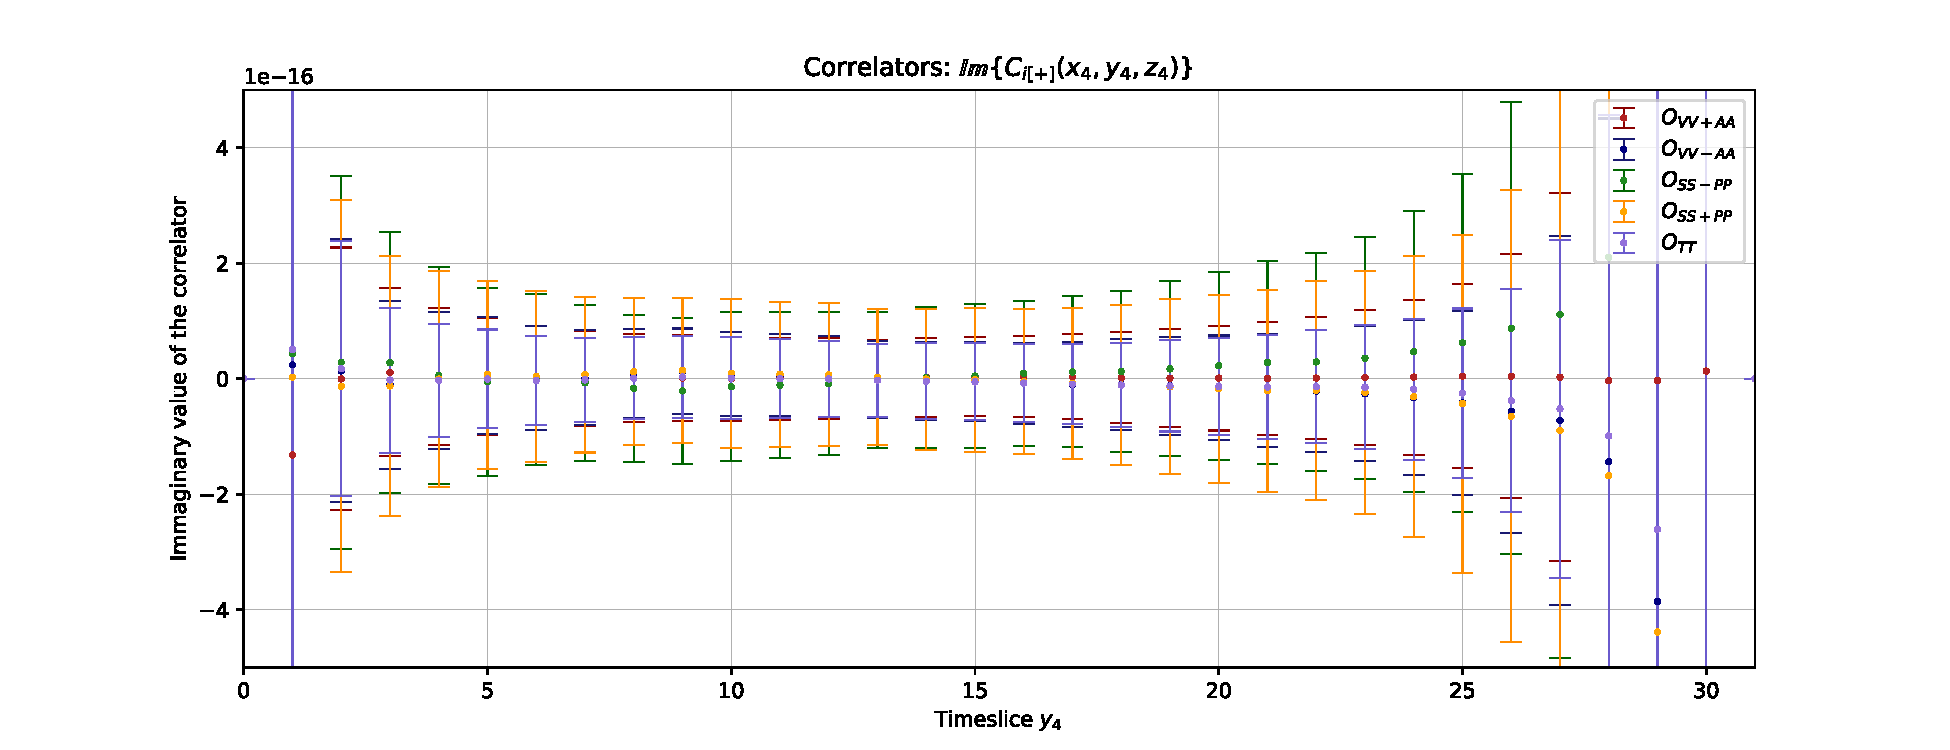
\includegraphics[width=\textwidth]{imgs-MSc-thesis/pureYM-immaginary.pdf}
    \caption{Test of simulation of three points correlators on a set of 54 quenched configurations, $\beta = 6.0$, tree level improved Symanzik gauge action.
        It has been used a \texttt{16x16x16x32} lattice.}
    \label{fig:reality3pts}
\end{figure}

\section{Proof of $\gamma_5 S_{(i,\pm)} (u,v) \gamma_5 = S_{(i,\mp)}^\dag (v,u)$}\label{app:proof-G5-DW}
\noindent
The starting point is a well known property of the Dirac-Wilson operator $D_W$: $\gamma_5 D_W(x,y) \gamma_5 = D_W^\dag(y,z)$.
The bilinear operator of the Osterwalder-Seiler theory is $D_W \pm i\gamma_5 \mu$, and the quark propagator is just its inverse:
\begin{equation*}
    \sum_z \left(D_W \pm i\gamma_5 \mu\right) (x,z) S_{(\pm)} (z,y) = \delta^{(4)}_{xy}
\end{equation*}
By multiplying $\gamma_5$ to the left, to the right and inserting a $\mathbb{I} = (\gamma_5)^2$ between the operator and the propagator:
\begin{equation*}
    \sum_z \left( D_W \mp i\gamma_5 \mu \right)^\dag (z,x) \left[\gamma_5 S_{(\pm)} (z,y) \gamma_5\right] = \delta^{(4)}_{xy}
\end{equation*}
Now I remember that $D_W$ doesn't contain the usual derivatives, but only terms like $\delta^{(4)}_{x;y+\hat\mu}$ or $\delta^{(4)}_{x;y-\hat\mu}$.
In other words, the Dirac-Wilson operator on the lattice is just a matrix.
Then it can be exchanged with other matrices $M$ - i.e. $D_W (u,v) M(w,l) = M(w,l) D_W (u,v)$.
As a consequence:
\begin{equation*}
    \sum_z \left[\gamma_5 S_{(\pm)} (z,y) \gamma_5\right] \left( D_W \mp i\gamma_5 \mu \right)^\dag (z,x) = \delta^{(4)}_{yx}
\end{equation*}
The term $\gamma_5 S_{(\pm)} (z,y) \gamma_5$ it is clearly $S_{(\mp)}^\dag (y,z)$ for definition.
\proved
\section{Proof of connection of Gauge fields space}\label{app:connection}
\noindent
The proof of the connection of the $SU(3)$ Gauge field space is reported below and taken from \cite{OBC_top}.
The proof is based on the continuum theory.
Because of the mentioned theorem in \cite{Topology-WilsonFlow-HMC}, for $a \rightarrow 0$ the lattice space of Gauge fields tends to have the same topological connection properties of the one described below.
\newline\newline
\textit{$(*)$ proof:}
\newline
It is well known that Gauge potentials $A_\mu (x)$ can be described as $\text{End}(E)-$valued 1-forms, where $E$ is the $G-$bundle over a smooth manifold $M$ \cite{Baez}.
In this case $M$ is the manifold obtained from the following product of spaces: $M = [0,T]\times \mathbb{T}^3$ and $\mathbb{T}^3$ is the three dimensional torus, topologically equivalent to the space $[0,L]\x[0,L]\x[0,L]$ with periodic boundary conditions.
\newline
In the paper by Luscher \cite{OBC_top} there is an interesting statement: ``since $M$ is contractible to a three dimensional torus, all $SU(3)$ principal bundles oer $M$ are trivializable''.
A direct consequence of this {\it global} trivialization is that Gauge fields are globally defined over all the manifold $M$.
\newline
At this point, the proof is essentially complete.
I must check that, given two Gauge fields $A_\mu^{(1)}$ and $A_\mu^{(2)}$, there always exists a smooth path in the fields space which connects them.
The proof is divided in three parts:
\newline
\newline
$(i)$ \textit{Each $A_\mu$ can be continously deformed to another ${A}_\mu'$ in temporal Gauge.}
\newline
It is defined a family of Gauge transformations $\Lambda_s (x), s\in [0,1]$ satisfying the following conditions:
$$\left(\partial_4 + sA_4 (x)\right) \Lambda_s^{-1} (x) = 0$$
$$\Lambda_0 (x) \big|_{x_4 = 0} = \mathbb{I}_3$$
I apply the Gauge transformation to a generic $A_\mu (x)$ that satisfies \obc.
I must prove that the transformed field $A_\mu^s (x)$ satisfies the temporal gauge and it still has \obc\space.
\begin{equation*}
    A_\mu^s (x) = \Lambda_s (x) A_\mu (x) \Lambda_s^{-1} (x) + \Lambda_s (x) \partial_\mu \Lambda_s^{-1} (x) 
\end{equation*}
\begin{itemize}
    \item Temporal Gauge in $s=1$: $$A_4^0 (x) = \Lambda_1 (x) A_4 (x) \Lambda_1^{-1} (x) - \Lambda_1 (x) A_4 (x) \Lambda_1^{-1} (x) = 0$$
    \item \obc\space $\forall s \in [0,1]$: I perfectly know how the strength tensor transforms under Gauge transformations:
        $$F_{\mu\nu} (x) \mapsto F_{\mu\nu}^s (x) = \Lambda_s (x) F_{\mu\nu} (x) \Lambda_s^{-1} (x) $$
        Then it is trivial to assert that $F_{0i}^s (\vec x, 0) = F_{0i}^s (\vec x, T) = 0$.
        The transformed fields satify \obc.
\end{itemize}
$(ii)$ \textit{Each $A_\mu$ in temporal Gauge can be contracted to the null Gauge field $A_\mu = 0$.}
\newline
This part of the proof is trivial: I choose te path $A_\mu^s = s\cdot A_\mu$
\newline\newline
At this point it is proven that each $A_\mu$ satisfying \obc\space can be smoothly contracted to the null potential.
Then each couple of potentials $A_\mu^{(1)}$ and $A_\mu^{(2)}$ satisfying \obc\space are connected in the fields space.
\proved

\section{Pseudoscalar propagator with OBC}\label{app:sinh-proof}
\noindent
I want to derive the form of the propagator (\ref{eq:sinh}) in presence of \obc\space on fermion fields.
For simplicity, I work the calculation in continuum QCD.
First of all, I must derive the boundary conditions on pseudoscalar mesons.
I do it by looking at appendix \ref{app:proof-reality}: the generic pseudoscalar meson operator is proportional to the pseudoscalar density $P^{ab}(x)=\bar \psi^a (x) \gamma_5 \psi^b (x)$
Then I can infere its boundary conditions from the conditions in the fermion fields (\ref{eq:obc-on-fermions}).
\newline
I can write the identity in the following way $\mathbb{I}_4 = P_+ + P_-$.
Then I can insert it in a pseudoscalar density evaluated in $x_4 = 0$:
\begin{equation*}
    \bar\psi^a \gamma_5 \psi^b \Big|_0 = \bar\psi^a \gamma_5 (P_+ + P_-) \psi^b \Big|_0 = \bar\psi^a \gamma_5 P_- \psi^b \Big|_0 =
\end{equation*}
now I make use of time reflection symmetry:
\begin{equation*}
    \mathbb{T}: 
    \begin{cases}
        \psi (\vec x, x_4) \mapsto - \gamma_1 \gamma_3 \psi (\vec x,T-x_4) \\
        \bar \psi (\vec x, x_4) \mapsto - \bar\psi (\vec x,T-x_4) \gamma_3 \gamma_1 \\
    \end{cases}
\end{equation*}
thus:
\begin{equation*}
    = (-)^2 \bar\psi^a \gamma_3 \gamma_1 \gamma_5 P_- \gamma_1 \gamma_3 \psi^b \Big|_T = \bar\psi^a \gamma_5 \gamma_3 \gamma_1 \gamma_1 P_+ \gamma_3 \psi^b \Big|_T = \bar\psi^a \gamma_5 \gamma_3 \gamma_3 P_- \psi^b \Big|_T = 0
\end{equation*}
the same holds for the case $x_4 = T$. Then the boundary conditions on the pseudoscalar densities are:
\begin{equation}\label{obc-on-pions}
    P^{ab} (\vec x , 0) = P^{ab} (\vec x , T) = 0 \hspace*{1cm} \forall a,b = 1,2,3
\end{equation}
To simplify the notation, I will use $\pi$ to refer to the generic $P^{ab}$.
\newline
In first order of Chiral Perturbation Theory, the generic pion satisfies the Klein Gordon equation, that in euclidean notation reads\footnote{here the variables $t,t'$ are the euclidean times $x_4, y_4$.}:
\begin{equation*}
    \left(-\frac{\partial^2}{\partial t^2} - \nabla_3^2 + m^2 \right) \pi(\vec x,t) = 0
\end{equation*}
where $\nabla_3^2$ is the Laplace operator in $\mathbb{E}^3$.
A generic non homogeneous equation can be solved by using the associated Green function that must satisy the same boundary conditions of the field \cite{zaffaroni-pradisi}.
The spatial part of the equation is solved through the Fourier transform method (as done in every course of quantum field theory) and helps to reduce the equation for the Green function in this way:
\begin{equation*}
    \left(-\frac{\partial^2}{\partial t^2} - \vec p^2 + m^2 \right) G_\omega(t,t') = \left(-\frac{\partial^2}{\partial t^2} - \omega^2 \right) G_\omega(t,t') = L_\omega G_\omega(t,t') = 0
\end{equation*}
Notice that, in this case, we do not have $G_\omega(t-t')$ but $G_\omega(t,t')$ because these boundary conditions, unlike the periodic ones, break the time translation invariance.
The generic solution is:
\begin{equation*}
    G_\omega(t,t') = \theta (t-t')\phi^\text{sup}(t)\alpha (t') + \theta (t'-t) \phi^\text{inf}(t)\beta (t')
\end{equation*}
where:
\begin{equation*}
    \begin{cases}
        L_\omega \phi^\text{sup} (t) = 0 \\
        \phi^\text{sup} (T) = 0
    \end{cases}
    \quad \text{ and } \quad
    \begin{cases}
        L_\omega \phi^\text{inf} (t) = 0 \\
        \phi^\text{inf} (0) = 0
    \end{cases}
\end{equation*}
with this choice the boundary conditions are automatically satisfied.
The coefficients $\alpha (t')$ and $\beta (t')$ must be chosen in order to make $G_\omega(t,t')$ continous and its first derivative must be an Heaviside $\theta(t-t')$.
By imposing these conditions I found:
\begin{equation*}
    \begin{aligned}
        G_\omega (t,t') = & \theta (t-t') \frac{\sinh \left( \omega (T - t) \right) \cdot \sinh \left( \omega t' \right)}{2 \omega \sinh \left( \omega T \right)} + \\
                          & + \theta (t'-t) \frac{\sinh \left( \omega (T - t') \right) \cdot \sinh \left( \omega t \right)}{2 \omega \sinh \left( \omega T \right)}
    \end{aligned}
\end{equation*}
Then I remember that $G_\omega(t,t') = \tilde G(\vec p,t,t')$, the propagator in three-momentum space and euclidean time. The summation over spatial coordinates will set $\vec p=0$ as outlined in section \ref{sec:asympt-behav}.
\proved

\backmatter
\phantomsection
\printbibliography

%Ringraziamenti
\begin{acknowledgments}
    Finalmente la pagina conclusiva che, per rispetto della lingua inglese, scriverò in italiano.
    Anzi, inzio scusandomi proprio con gli inglesi.
    \newline\newline
    Il primo ringraziamento va alla mia famiglia: a mamma, papà, Erika e Gabriele.
    Voi conoscete la parte meno bella dell'essere una persona così appassionata per questo mondo: ore al PC curvo sulla scrivania e sacchi di irritabilità.
    Grazie per avermi sopportato.
    Grazie per aver sostenuto ogni scelta della mia vita, assicurandovi che fossero scelte che mi rendessero felice e soddisfatto; e per avermi lasciato sbagliare, quando necessario.
    Senza di voi non so come farei.
    \newline\newline
    Un ringraziamento va al mio relatore, il Prof. Mauro Papinutto, che si è dimostrato molto più disponibile di quanto io stesso mi aspettassi.
    La ringrazio in particolar modo per non aver badato a spese in termini di tempo: spiegazioni lunghe ore, risposte ad email sotto le feste, etc.
    Questi mesi sotto la sua supervisione sono stati estremamente formativi, sia dal punto di vista scientifico ma soprattutto dal punto di vista di approccio alla fisica.
    Grazie.
    \newline\newline
    Ringrazio Chiara per avermi ospitato durante i suoi tanti viaggi in giro per l'Europa.
    Penso che tu sia la persona che più di ogni altra mi capisce e siamo arrivati al punto in cui ormai certe cose nemmeno ce le diciamo, le capiamo e basta
    Grazie per quest'amicizia spensierata, per quei momenti di tranquillità e distacco dal mondo, per avermi inseganto più di quanto credi.
    Grazie per avermi fatto capire che con il giusto mix di incoscienza e determinazione si può fare di tutto.
    \newline\newline
    Ringrazio tutti i miei amici storici: Emanuele, Sirio, Gianmarco, Gaia, Andrea, Martina, Mariachiara, Adriana e Alice.
    A prescindere da quanto tempo passi e da quanto non ci si veda, stare con voi è sempre come avere 10 anni e credo che questa sia una cosa bellissima.
    \newline\newline
    Ringrazio i miei amici di Fisica, che purtroppo sono quasi tutti assenti perché ormai sparsi per il mondo a fare i ricercatori.
    In particolare Daniele Migliorati, Marcello Romano, Pierfrancesco Martini, Giulia Muco, Pietro Moroni, Giulio Marino e Michele Tortora.
    Stare accanto a voi è stato incredibilmente stimolante e starvi dietro continua ad essere una grandissima sfida per me.
    Grazie mille.
    \newline\newline
    Grazie ad Aurora e Gabriele per tutti i bei momenti che abbiamo passato insieme, ma soprattutto grazie per essere gli unici in questa lunga lista di persone a cui piace andare a mare!
    \newline\newline
    Grazie a Marco per essere il mio coach di vita, per essere d'esempio, soprattutto cattivo esempio!
    Grazie a Iole per tutte le volte che pensavi che ti stessi supportando quando in realtà ti stavo solo prendendo in giro.
    Grazie a Claudio per la passione che mi hai trasmesso, per la fiducia che mi hai dato e per gli scossoni nei momenti incerti.
    Grazie a Sara per essere il CG che tutti vorremmo e per portarti sempre dietro un sorriso, anche quando ci sarebbe solo che da' piagne!
    \newline\newline
    Ringrazio tutta la comunità scientifica che nel tempo ha dedicato energie, denaro, tempo, impegno in qualcosa che, in ogni epoca, sembrava sempre inutile e poco pratica.
    Mi date speranza.
    Credo che non ci sia nulla di più soddisfacente dello scoprire i meccanismi dietro al mondo.
    \newline\newline
    Credo che dietro ogni scienziato si nasconda del romanticismo.
\end{acknowledgments}

\end{document}
